\documentclass[openany]{book}

\usepackage{amssymb}            % For mathematical symbols
\usepackage{amsmath}            % For, say, math operators I guess
\usepackage[title]{appendix}    % For appendices. May or may not be required.
\usepackage{booktabs}           % For tables, mainly the \toprule \midrule \bottomrule
\usepackage{graphicx}           % Required for inserting images
\usepackage{hyperref}           % For hrefs
\usepackage{listings}           % For verbatim R code chunks
\usepackage{multirow}           % For, as you can guess, multirows
\usepackage{natbib}             % For bibliography
\usepackage{url}                % For bare url links
\usepackage[svgnames]{xcolor}   % For colouring text
\usepackage{xfrac}              % For inline fractions, advised by: https://tex.stackexchange.com/questions/128496

\title{Thesis draft}
\author{Leonardo Cefalo}

\begin{document}

\maketitle
\tableofcontents
%
% 
%
%% ------------------------------------------------------------------------------ %%
%% --------                   First Chapter                 --------------------- %%
%% ------------------------------------------------------------------------------ %%
\chapter[INLA]{The INLA and Gaussian Markov Random Fields} \label{chapter:INLA}
%
%% -------- Introduction --------------------------------- %%
\section{Introduction}
In this chapter, we present an overview of a computational methodology extensively used throughout this thesis, the Integrated Nested Laplace Approximation. 

In the context of Bayesian inference, integrating out the posterior distribution of the parameters of interest only happens in a small number of fortunate cases, i.e. when among all possible prior distributions, a set of conjugate ones is assumed. 

The most popular way to overcome non-conjugacy in the posteriors is the approximation of posteriors by simulation using Markov Chain Monte Carlo (MCMC hereinafter) methods. MCMC methods are a true institution in Bayesian statistics due to their rigorous background and the capability of balancing computational speed and accuracy.

Nevertheless, an alternative approach has emerged in the last seventeen years, the Integrated Nested Laplace Approximation \citep[][INLA hereinafter]{INLA, VBINLA}. The core idea behind INLA is to directly apply a deterministic approximation to the posterior, and dates back to the proposal by \cite{tierney1986accurate} to approximate the first and second moments of the parameters. The Laplace approximation leverages on the convergence of the full posterior to a Gaussian distribution when parameters are Gaussian \textit{a priori}, the approximation error being in $\mathcal{O}(n^{-1})$ where $n$ is the length of the target variable. 

The most convenient area of application of INLA are the models for Gaussian Markov Random Fields \citep{GMRFs}, due to the computational properties we describe in Section \ref{section:GMRFs}. That being said, the remainder of this chapter will briefly summarise how the INLA works in Section \ref{section:inla} and the \texttt{R} software in which it is implemented in Section \ref{section:r_inla}



%% -------- Why Using GMRFs? ----------------------------- %%
\section[GMRFs]{Why using INLA? Gaussian Markov Random Fields}\label{section:GMRFs}

\subsection{Conditional Independence in Gaussian Random Fields}\label{par:GRFs}
A fundamental property of the Normal distribution is that if two observations are mutually independent conditioned on all the other ones, then their marginal precision element is zero even though their marginal covariance is nonzero \cite{GMRFs}.

To see this, consider a generic $n$-dimensional Gaussian random field $\mathbf{X} = (X_1, X_2 .. . X_n) \sim N(\mathbf{\mu}, \mathbf{\Sigma})$. Then, a deductive prove is given for the property:
\begin{equation}
		X_i \bot X_j \mid \mathbf{X_{-ij}} \iff q_{ij} = 0
		\label{eq:theorem1}
\end{equation}

For any $i \neq j,  \quad i \leq n, \quad j\leq n$; $q_{i,j}$ is the element in position $(i,j)$ in the precision matrix $\mathbf{Q}: = \mathbf{\Sigma^{-1}}$, assuming that $\mathbf{\Sigma}$ is nonsingular. Any set of indexes $A \subset \mathbb{N}^n$ can be chosen in order to partition $\mathbf{X}$ into $\mathbf{X_A}$ and $\mathbf{X_B}$, being $B = \mathbb{N}^n / A$ with $card(A) := m<n, \, card(B) = n-m$, namely:
	$$
	\mathbf{X} := \left( \begin{array}{l} \mathbf{X_A} \\ \mathbf{X_B}
		\end{array}
	\right)  , \quad 
		\mathbf{\mu} = \left( \begin{array}{l} \mathbf{\mu_A} \\ \mathbf{\mu_B}
	\end{array}
	\right)
	 \,\, \text{and} \quad 
	\mathbf{\Sigma} = \left( \begin{array}{ll} \mathbf{\Sigma_{AA}} & \mathbf{\Sigma_{AB}}
		 \\ \mathbf{\Sigma_{BA}} & \mathbf{\Sigma_{BB}}
	\end{array}
	\right)
	$$
    
Clearly the $\mathbf{\Sigma_{AA}}$ has dimensions $m \times m$, $\mathbf{\Sigma_{BB}}$ is $(n-m) \times (n-m)$,	$\mathbf{\Sigma_{AB}}$ is $n \times (n-m)$ and $\mathbf{\Sigma_{BA}} = \mathbf{\Sigma'_{AB}}$. 
Since $\mathbf{X}$ is Gaussian by definition, we know its density is

$$ \pi(\mathbf{X}) = \frac{1}{(2 \pi)^{n/2} \mid \mathbf{\Sigma} \mid ^{-1}} \, \, e^{-\frac{d^2}{2}}, \quad \text{with} \quad  d^2 := (\mathbf{X} - \mathbf{\mu})' \mathbf{\Sigma}^{-1} (\mathbf{X} - \mathbf{\mu}) $$

Being $d^2$ the squared Mahalanobis distance. From the law of compound probability we also know that 
    
    $$\pi(\mathbf{X}) = \pi(\mathbf{X_A}|\mathbf{X_B}) \, \pi(\mathbf{X_B}) \quad \text{or equivalently} \quad \ln \pi(\mathbf{X}) = \ln \pi(\mathbf{X_A}|\mathbf{X_B}) + \ln \pi(\mathbf{X_B})$$ 


 Since $\pi(\mathbf{X}) \propto exp(-\tfrac{d^2}{2})$, this implies that $d = d^2_{A|B} + d^2_{B}$, being $d^2_{A|B}$ and $d^2_B$ the squared Mahalanobis distances of respectively the conditional distribution of $\mathbf{X_A}$ given $\mathbf{X_B}$ and the marginal distribution of $\mathbf{X_B}$.
  
 To compute the precision matrix $\mathbf{Q} := \mathbf{\Sigma^{-1}}$, we keep treating $\mathbf{\Sigma}$ as a block matrix and decompose it into three matrices of the same size whose inversion is somewhat easier. Specifically we want to factorise $\mathbf{\Sigma}$ as $\mathbf{T_U} \times \mathbf{C} \times \mathbf{T_L}$, where $\mathbf{T_L}$ and $\mathbf{T_U}$ are respectively a lower triangular and an upper triangular matrix; $\mathbf{C}$ instead must have zeroes as the upper right and lower left blocks. Let us start by defining:
 $$
  \mathbf{T_L} = \left( \begin{array}{ll} 
 	\mathbf{I} & \mathbf{0}\\ 
 	\mathbf{\Sigma_{BB}^{-1}} \mathbf{\Sigma_{BA}} & \mathbf{I}
 \end{array}
 \right)
$$ 
which allows us to factorise $\mathbf{\Sigma}$ in this way:

$$
\mathbf{\Sigma} = \left( \begin{array}{ll} \mathbf{\Sigma_{AA}} & \mathbf{\Sigma_{AB}}
	\\ \mathbf{\Sigma_{BA}} & \mathbf{\Sigma_{BB}}  \end{array}
\right) = 
\left( \begin{array}{ll} \mathbf{\mathbf{\Sigma_{AA}} - \mathbf{\Sigma_{AB}} \mathbf{\Sigma^{-1}_{BB}} \mathbf{\Sigma_{BA}}} & \mathbf{\Sigma_{AB}}
	\\ \mathbf{0} & \mathbf{\Sigma_{BB}}  \end{array}
\right)
\left( \begin{array}{ll} 
	\mathbf{I} & \mathbf{0}\\ 
	\mathbf{\Sigma_{BB}^{-1}} \mathbf{\Sigma_{BA}} & \mathbf{I}
\end{array}
\right)
$$
For the sake of simplicity, we set 
$$\mathbf{S_{BB}} : =
\mathbf{\Sigma_{AA}} - \mathbf{\Sigma_{AB}} \mathbf{\Sigma^{-1}_{BB}} \mathbf{\Sigma_{BA}}
$$
This term is referred to as the Schur's complement of $\mathbf{\Sigma_{BB}}$ in $\mathbf{\Sigma}$ \citep[][paragraph 0.7.3]{HornJohnson}. A crucial assumption is that this matrix is nonsingular.

The left factor in the above formula is factorised as:

$$
 \left( \begin{array}{ll} \mathbf{S_{BB}}  & \mathbf{\Sigma_{AB}}
	\\ \mathbf{0} & \mathbf{\Sigma_{BB}}  \end{array}
\right) 
 =  \left( \begin{array}{ll} 
	\mathbf{I} &  \mathbf{\Sigma_{AB}} \mathbf{\Sigma_{BB}^{-1}}
	\\ \mathbf{0} & \quad \mathbf{I} \quad
\end{array}
\right)
\left( \begin{array}{ll} 
	\mathbf{S_{BB}}   & \mathbf{0}\\ 
	\mathbf{0}  & \mathbf{\Sigma_{BB}}
\end{array} \right)
$$
with
$$ \mathbf{T_U} =
\left( \begin{array}{ll} 
	\mathbf{I} &  \mathbf{\Sigma_{AB}} \mathbf{\Sigma_{BB}^{-1}}
	\\ \mathbf{0} & \quad \mathbf{I} \quad
\end{array}
\right)  \quad \text{and} \quad \mathbf{C} =
\left( \begin{array}{ll} 
	\mathbf{S_{BB}}   & \mathbf{0}\\ 
	\mathbf{0}  & \mathbf{\Sigma_{BB}}
\end{array} \right) 
$$



 so that:
$$
\mathbf{\Sigma} = \mathbf{T_U} \, \mathbf{C} \, \mathbf{T_L} =
 \left( \begin{array}{ll} 
	\mathbf{I} &  \mathbf{\Sigma_{AB}} \mathbf{\Sigma_{BB}^{-1}}
	\\ \mathbf{0} & \quad \mathbf{I} \quad
\end{array}
\right)
\left( \begin{array}{ll} 
	\mathbf{S_{BB}}   & \mathbf{0}\\ 
	\mathbf{0}  & \mathbf{\Sigma_{BB}}
\end{array} \right)
\left( \begin{array}{ll} 
	\mathbf{I} & \mathbf{0}\\ 
	\mathbf{\Sigma_{BB}^{-1}} \mathbf{\Sigma_{BA}} & \mathbf{I}
\end{array}
\right)
$$
It follows straightforwardly that:
$$
\mathbf{T_U^{-1}} =  
\left( \begin{array}{ll} 
	\mathbf{I} & - \mathbf{\Sigma_{AB}} \mathbf{\Sigma_{BB}^{-1}}
	\\ \mathbf{0} & \quad \mathbf{I} \quad
\end{array}
\right), \quad
\mathbf{T_L^{-1}} = 
\left( \begin{array}{ll} 
	\quad \mathbf{I} & \mathbf{0}\\ 
	- \mathbf{\Sigma_{BB}^{-1}} \mathbf{\Sigma_{BA}} & \mathbf{I}
\end{array}
\right)
$$ and $$
\mathbf{C}^{-1} = 
\left( \begin{array}{ll} 
	\mathbf{S_{BB}^{-1}}   & \mathbf{0}\\ 
	\mathbf{0}  & \mathbf{\Sigma_{BB}^{-1}}
\end{array} \right)
$$
Thus we derive this general result, which holds for any distribution, provided that marginal covariance matrices are nonsingular:
\begin{equation}
	\mathbf{Q} = \mathbf{\Sigma}^{-1} = 
	\left( \begin{array}{ll} 
		\quad \mathbf{I} & \mathbf{0}\\ 
		- \mathbf{\Sigma_{BB}^{-1}} \mathbf{\Sigma_{BA}} & \mathbf{I}
	\end{array}
	\right)
	\left( \begin{array}{ll} 
		\mathbf{S_{BB}^{-1}}   & \mathbf{0}\\ 
		\mathbf{0}  & \mathbf{\Sigma_{BB}^{-1}}
	\end{array} \right)
    \left( \begin{array}{ll} 
    	\mathbf{I} & - \mathbf{\Sigma_{AB}} \mathbf{\Sigma_{BB}^{-1}}\\ 
    	\mathbf{0} & \quad \mathbf{I} \quad
    \end{array} \right)
\label{eq:precision1}
\end{equation}
If we perform the multiplication we obtain
$$
\mathbf{Q} = 
	\left( \begin{array}{ll} 
	\mathbf{S_{BB}^{-1}}   &
	\mathbf{S_{BB}^{-1}} \mathbf{\Sigma_{AB}} \mathbf{\Sigma_{BB}^{-1}}\\ 
	\mathbf{\Sigma_{BB}^{-1}} \mathbf{\Sigma_{AB}} \mathbf{S_{BB}^{-1}}& 
	\mathbf{\Sigma_{BB}^{-1}} + \mathbf{\Sigma_{BB}^{-1}} 
	\mathbf{\Sigma_{BA}} \mathbf{S_{BB}^{-1}}
    \mathbf{\Sigma_{AB}} \mathbf{\Sigma_{BB}^{-1}} 
\end{array} \right)
$$

As for $\mathbf{S_{BB}}$, we may define:
$\mathbf{S_{AA}} : =
\mathbf{\Sigma_{BB}} - \mathbf{\Sigma_{BA}} \mathbf{\Sigma^{-1}_{AA}} \mathbf{\Sigma_{AB}}$ and notice that
$$
\left(\mathbf{\Sigma_{BB}^{-1}} + \mathbf{\Sigma_{BB}^{-1}} \mathbf{\Sigma_{BA}} \mathbf{S_{BB}^{-1}}
\mathbf{\Sigma_{AB}} \mathbf{\Sigma_{BB}^{-1}} \right) \, \, 
\left(\mathbf{\Sigma_{BB}} - \mathbf{\Sigma_{BA}} \mathbf{\Sigma^{-1}_{AA}} \mathbf{\Sigma_{AB}} \right) =
$$
$$
= \mathbf{I} 
- \mathbf{\Sigma_{BB}^{-1}} \mathbf{\Sigma_{BA}} \mathbf{\Sigma_{AA}^{-1}} \mathbf{\Sigma_{AB}}
+ \mathbf{\Sigma_{BB}^{-1}} \mathbf{\Sigma_{BA}} \mathbf{S_{BB}^{-1}}
  \mathbf{\Sigma_{AB}} 
- \mathbf{\Sigma_{BB}^{-1}} \mathbf{\Sigma_{BA}}      \mathbf{S_{BB}^{-1}}
  \mathbf{\Sigma_{AB}}      \mathbf{\Sigma_{BB}^{-1}} \mathbf{\Sigma_{BA}}
  \mathbf{\Sigma^{-1}_{AA}} \mathbf{\Sigma_{AB}} = 
$$
$$
= \mathbf{I} - \mathbf{\Sigma_{BB}^{-1}} \mathbf{\Sigma_{BA}} \,
\left( \mathbf{S_{BB}^{-1}}  - \mathbf{S_{BB}^{-1}}  \mathbf{\Sigma_{AB}}      \mathbf{\Sigma_{BB}^{-1}} \mathbf{\Sigma_{BA}}
\mathbf{\Sigma^{-1}_{AA}} - \mathbf{\Sigma^{-1}_{AA}} \right) \,
\mathbf{\Sigma_{AB}} =
$$ 
$$
\mathbf{I} - \mathbf{\Sigma_{BB}^{-1}} \mathbf{\Sigma_{BA}} \,
\left[
\mathbf{S_{BB}^{-1}} - \mathbf{S_{BB}^{-1}} \left(\mathbf{\Sigma_{AA}} - \mathbf{S_{BB}} 
 \right)\mathbf{\Sigma^{-1}_{AA}} - \mathbf{\Sigma^{-1}_{AA}}
\right] \, \mathbf{\Sigma_{AB}} = \mathbf{I}
$$
This enables us to write the precision matrix in compact form:
\begin{equation}
\mathbf{Q} = 
\left( \begin{array}{ll} 
	\mathbf{S_{BB}^{-1}}   &
	\mathbf{S_{BB}^{-1}} \mathbf{\Sigma_{AB}} \mathbf{\Sigma_{BB}^{-1}}\\ 
	\mathbf{\Sigma_{BB}^{-1}} \mathbf{\Sigma_{AB}} \mathbf{S_{BB}^{-1}}& 
	\mathbf{S_{AA}^{-1}}  
\end{array} \right)
\end{equation}
What matters is that the precision elements corresponding to the variables included in the subset $A$, namely $\mathbf{X_A}$ are all in the matrix $\mathbf{S_{BB}^{-1}}$.

Recalling equation \ref{eq:precision1}, it is possible to show a fundamental property of the Normal distribution \citep[][result 4.6]{JohnsonWichern}.
If $\mathbf{X}$ has been partitioned into sets $A$ and $B$, the squared Mahalanobis distance can be written as:
 
$$
 \begin{aligned}
	d^2 = 
	\left( \begin{array}{l} 
		\mathbf{X_A} - \mu_A\\
		\mathbf{X_B} - \mu_B
	\end{array} \right)'
	\left( \begin{array}{ll} 
		\quad \mathbf{I} & \mathbf{0}\\ 
		- \mathbf{\Sigma_{BB}^{-1}} \mathbf{\Sigma_{BA}} & \mathbf{I}
	\end{array}
	\right)
	\left( \begin{array}{ll} 
		\mathbf{S_{BB}^{-1}}   & \mathbf{0}\\ 
		\mathbf{0}  & \mathbf{\Sigma_{BB}^{-1}}
	\end{array} \right) \times
	\notag\\ \times
	\left( \begin{array}{ll} 
	\mathbf{I} & - \mathbf{\Sigma_{AB}} \mathbf{\Sigma_{BB}^{-1}}\\ 
	\mathbf{0} & \quad \mathbf{I} \quad
    \end{array} \right)
    \left( \begin{array}{l} 
    	\mathbf{X_A} - \mu_A\\
    	\mathbf{X_B} - \mu_B
    \end{array} \right)	 =
\end{aligned}
$$ 
$$ 
\begin{aligned}=
	\left( \begin{array}{l} 
	\mathbf{X_A} - \mu_A + (\mathbf{X_B} - \mu_B) \mathbf{\Sigma_{BB}^{-1}} \mathbf{\Sigma_{BA}}\\
	\mathbf{X_B} - \mu_B 
\end{array} \right)'
	\left( \begin{array}{ll} 
	\mathbf{S_{BB}^{-1}}   & \mathbf{0}\\ 
	\mathbf{0}  & \mathbf{\Sigma_{BB}^{-1}}
\end{array} \right) \times \\
\notag    \times
	\left( \begin{array}{l} 
	\mathbf{X_A} - \mu_A + (\mathbf{X_B} - \mu_B) \mathbf{\Sigma_{BB}^{-1}} \mathbf{\Sigma_{BA}}\\
	\mathbf{X_B} - \mu_B 
\end{array} \right)
\end{aligned}
$$ 

By setting $ \mu_{A|B} :=  \mu_A + (\mathbf{X_B} - \mu_B) \mathbf{\Sigma_{BB}^{-1}} \mathbf{\Sigma_{BA}}$ $d^2$ is decomposed into:

$$ d^2 = 
\left( \mathbf{X_A} - \mu_{A|B} \right)' \mathbf{S_{BB}^{-1}}\left( \mathbf{X_A} - \mu_{A|B}\right) + 
\left( \mathbf{X_B} - \mu_B \right)'\mathbf{\Sigma_{BB}^{-1}}\left( \mathbf{X_B} - \mu_B\right)
$$
 
The second term is $d_B^2$, namely the Mahalanobis distance for the partition $\mathbf{X_B}$. The first term is the Mahalanobis distance of a Normal distribution with mean $\mu_{A|B}$ and covariance $\mathbf{S_{BB}}$, but it must also be the Mahalanobis distance of $\mathbf{X_A}$ conditioned on $\mathbf{X_B}$, by the law of conditional probability. 
Therefore it is proved that, if $\mathbf{X} \sim N(\mathbf{\mu}, \mathbf{\Sigma})$, for any two partitons $A$ and $B$ such that $\mathbf{X_B}$ is the complement to $\mathbf{X_A}$ with respect to $\mathbf{X}$, then 

\begin{equation}
	\mathbf{X_A} | \mathbf{X_B} \sim N \left(
	\mu_A + (\mathbf{X_B} - \mu_B) \mathbf{\Sigma_{BB}^{-1}} \mathbf{\Sigma_{BA}}, \, \,
	 \mathbf{\Sigma_{AA}} - \mathbf{\Sigma_{AB}} \mathbf{\Sigma^{-1}_{BB}} \mathbf{\Sigma_{BA}}
	 \right)
	 \label{eq:Conditional_Normal}
\end{equation}

Now we can prove equation \ref{eq:theorem1}.
The partition $\mathbf{X_A}$ conditional to $\mathbf{X_B}$, has therefore precision equal to $\mathbf{S_{BB}^{-1}}$, according to equation (\ref{eq:Conditional_Normal}). Yet also the element of the joint precision matrix corresponding to the subset $A$ is equal to $\mathbf{S_{BB}^{-1}}$.
This means that by choosing the index set $A$ as any couple $(i,j)$ with $i \neq j$, we have

\begin{equation}
	\mathrm{COV}[X_i, X_j | \mathbf{X_{-ij}}] \equiv q_{ij} 
\end{equation}
And if these two variables are conditionally independent, then their precision element is zero, as stated in equation \ref{eq:theorem1}.  

Equation \ref{eq:theorem1} implies that modelling Gaussian processes with sparse precision matrix implies a gain in computation. 
\subsection{The Markov Property}
Section \ref{par:GRFs} shows that conditional pairwise independence in Gaussian random fields implies the corresponding marginal precision element is zero. 

It is thus convenient to identify a class of probabilistic models for Gaussian random fields for which conditional pairwise independence holds by definition. A sufficient condition to this aim is to satisfy the Markov property. Following \citep[][Section 2.2]{GMRFs}, a Markovian random field can be intuitively defined with respect to a graph; it is easy to notice that the graph structure is a common representation for data like time series or lattice (either regular or irregular, in any number of dimensions). 

We start by assuming that each \textcolor{red}{element} of an $n$-dimensional Gaussian random field can thus be associated with a node in a graph denoted as $\mathcal{G} :=(\mathcal{S}, \mathcal {E}) $, where $\mathcal{S} = \lbrace s_i \rbrace_{i=1}^n$ is the set of nodes of size $n$ and $\mathcal{E} := \lbrace (s_i, s_j) : s_j \in \partial s_i  \rbrace_{i,j=1}^n$ is the set of edges;  hereinafter $\partial s_i$ denotes the set of neighbours of node $s_i$, or equivalently the set of nodes \textit{connected with} node $s_i$. By convention, it is assumed that $s_i \notin \partial s_i$.

The \textcolor{red}{relationship} $X:\mathcal{S} \rightarrow \mathbb{R}^n$ is thus assumed to hold, and for brevity we will write $X_i$ in place of $X(s_i)$. The \textit{global} Markov property \citep{HammersleyClifford} means that:
%
\begin{equation}
\pi(X_i \mid X_{-i}) = \pi(X_i \mid \partial s_i)
    \label{eq:gMarkov}
\end{equation}
%
 For a generic probability density function $\pi$. %satisfying the positivity condition. $\pi(X) : \pi(X(s_i)) > 0 \quad \forall s_i \in \mathcal{S}$
 This property is relevant to our aims because it implies that
 $$
 X_i \bot X_j  \mid X_{-i} \quad \forall j \notin \partial s_i
 $$
i.e. the probability distribution of $X_i$ is uniquely specified by its neighbours, and $X_i$ is independent on any non neighbouring site.

Putting together the Markov property (Equation \ref{eq:gMarkov}) with the precision structure of Gaussian random fields when conditional pairwise independence holds (Equation \ref{eq:theorem1}) it becomes clear that random processes satisfying both the conditions, namely the \textit{Gaussian Markov Random Fields} are characterised by a precision matrix, say $\mathbf{Q}$ which only has nonzero entries corresponding to neighbouring pairs, namely $\mathrm{card}(\mathcal{E})$. \textcolor{red}{For autoregressive time series and processes defined on regular lattices $\mathrm{card}(\mathcal{E})$ is a multiple of $n$; for irregular lattices there is no such an exact relationship, still the number of edges is typically in $\mathcal{\Theta}(n)$ in connected graphs.}
%This property is fundamental in that marginal independence frequently occurs in the most simple statistical models. For instance, any autoregressive processes with a sufficiently small lag order satisfies this condition by definition. Consider an unidirected $AR(p)$ Gaussian process: $X_i = \varphi_1 X_{i-1} + \varphi_2 X_{i-2} + ... + \varphi_p X_{i-p} + \varepsilon_i$ with $\varepsilon_i \sim N(0,\sigma^2)$.

%If we choose any index $j$ falling outside the interval $[i-p, \, i]$, $X_j$ is independent on $X_j$. As a consequence, the $i$-th row or column of the precision matrix will only have $k$ nonzero entries. If we generalise this consideration to all the realizations of the process, we see how the precision matrix only has $O(n)$ diagonal or off-diagonal nonzero values though it is an $n \times n$ matrix, so it is sparse. However, the covariance matrix does not include zeroes unless particular constraints are imposed.



%% -------- INLA summary --------------------------------- %%
\section{Introduction to the INLA}\label{section:inla}

\subsection{Latent Gaussian model outline}\label{par:LGM}
The baseline of how the INLA applies to our aims is a generic hierarchical regression model:
$$
\left\{ \begin{array}{ll} 
E[y\mid \eta, \Psi] = g^{-1}(\eta)\\
\eta = A \vartheta
\end{array} \right. 
$$
where $y$  denotes the response variable consisting of $N$ observations; $\eta$ is the linear predictor linked with a function $g$ to the expected value of the response variable; $\vartheta$ is a generic vector of latent variables of interest; $A$ is a known design matrix; $\Psi$ is the array of hyperparameters, whose size is usually in $\mathcal{O}(10^1)$. 

The linear predictor, to our aims, can be defined as:
$$  
\mathbf{A} := \left(X \quad \xi \right) \quad \text{and} \quad
\vartheta := \begin{pmatrix} \beta \\ \mathbf{z} \end{pmatrix}
$$
where $\beta$ is the array of regression coefficients of length $p$, $z$ is an additional array of latent effects of length $n$, $X$ is a matrix of explanatory variables of size $N \times p$, and $\xi$ is the design matrix of latent effects of size $N \times n$.

Labelling $\beta$ as "fixed" and $z$ as "random" effects is quite frequent in hierarchical regression applications, but due to the polysematic nature of these terms we will tend to avoid them. In a strictly probability perspective, there is no conceptual distinction between them: they are both unknown random variables entering the linear predictor through a known design matrix (either $X$ or $\xi$), are typically assumed to be Gaussian \textit{a priori} and their posterior distribution is the primary aim of statistical inference. We keep them separated due to how they are interpreted: $\beta$ represents the association between a set of known variables ($X$) and $y$, while $z$ is an unobserved process shaping the structure of $y$ itself.

%in order to map each observed value $y_j$ to one realisation of the random effect $z_i$, i.e. if $y_j$ depends on $z_i$ and therefore $\xi_{ji} = 1$, then  $y_j \perp\!\!\!\perp  z_{-i}$, with $i \in [1, n]$ and $j \in [1, N]$, where each row of $\xi$ has exactly one entry equal to $1$ and all other entries equal to $0$. 

The first necessary assumption is that $(y_j\perp\!\!\!\perp y_k )|\vartheta, \Psi$ and $(y_j\perp\!\!\!\perp \eta_k )|\vartheta, \Psi$ for any $j,k \in [1, N]$ with $j \neq k$, hence each observation $y_j$ depends on $\vartheta$ only through one value $\eta_j$. This also implies that the likelihood can be factorised as follows:
$$
f(y|\vartheta, \Psi) = f(y| \eta, \Psi) = \prod_{j = 1}^N f(y_j | \eta_j, \Psi)
$$
Moreover, we assume that $\vartheta$ follows a Normal distribution conditioned on $\Psi$; in our case, we have 
$$
\vartheta | \Psi \sim N(\mathbf{0}, (\mathbf{Q}_{\Psi})^{-1})
$$
where $\mathbf{Q}_{\Psi}$ denotes the precision matrix. Assuming that $\vartheta$ satisfies the Markovian properties is not necessary but it ensures the computational gains implied by the sparsity of $\mathbf{Q}_{\Psi}$.




%%%%% THIS IS ONLY VALID IN THE CLASSIC MODE OF R-INLA; namely, if $m$ is the size of $\vartheta$ (in this case, $m = N + n + p$), then the number of nonzero entries in $\mathbf{Q}$ is in $\mathcal{\vartheta}(m)$, i.e. in the same order of magnitude of $m$. The linear predictor is included in $\vartheta$ for computational reasons; with the appropriate choice of the stochastic representation of $\eta$ (see e.g. \cite{INLA2017}) if all other parameters are GMRFs, then $\vartheta$ is a GMRF as a whole. \\
Posterior marginals, namely $\pi(\vartheta_i | y)$ and $\pi(\Psi_j | y)$  $\forall i \in [1, n+p]$ and $j \in [1, \mathrm{card}(\Psi)]$, are obtained by solving the integrals:
 \begin{equation}
 \label{eq:marginals}
 \begin{aligned}
 %\left\{ \begin{array}{ll}
 \pi(\vartheta_i | y) = \int_{\Psi} \pi(\vartheta_i | y, \Psi) \pi(\Psi | y) d \Psi\\
 \pi(\Psi_j|y) = \int_{\Psi_{-j}} \pi(\Psi | y) \, d\Psi_{-j}
 %\end{array} \right.
 \end{aligned}
 \end{equation}
which is feasible provided that $\Psi$ has a small size. However, how we will see in the next paragraph, this operation can hardly be completed in closed form.



\subsection{Approximating Hyperparameters Posterior} \label{par:inla_psi}
Given Equation \ref{eq:marginals}, the first task is computing
 $$
\pi(\Psi | y) =  \frac{f(y | \eta, \Psi) \pi(\vartheta | \Psi) \pi(\Psi)}
{\pi(\vartheta | y, \Psi)f(y)} 
 $$
 
 The numerator is known \textit{a priori}; $f(y)$ does not depend on the parameters of interest and can be treated here as a normalising constant. The function which is hardly available in closed form, instead, is the full conditional $f(\vartheta | y, \Psi)$. 
 
 Thus, the idea behind the INLA it to replace it with its Gaussian approximation:
\begin{equation}
\label{eq:GaussianApprox}
\pi(\vartheta | y, \psi) \approx \pi_{G}(\vartheta | y, \psi) = \frac{\pi(\vartheta, y | \Psi)}{\int \pi_G(\vartheta, y | \Psi) \, d\vartheta}
\end{equation}

Where the subscript $G$ denotes the Gaussian approximation. For brevity, define $g(\vartheta) := ln \pi(\vartheta, y | \Psi)$. Then, a Taylor approximation truncated at the second order is applied:
\begin{align*}
g(\vartheta) \approx   g(\vartheta_0) + \nabla   g(\vartheta_0)'(\vartheta - \vartheta_0)+ \frac{1}{2}
(\vartheta - \vartheta_0)'H_g(\vartheta_0)(\vartheta - \vartheta_0)
\end{align*}

%\begin{align*}
%g(\vartheta) \approx \ln \pi(\vartheta_0, y | \Psi) + \nabla \ln \pi(\vartheta_0, y | \Psi)'(\vartheta - \vartheta_0)+ %\frac{1}{2}
%(\vartheta - \vartheta_0)'H \ln \pi(\vartheta_0, y | \Psi)(\vartheta - \vartheta_0)
%\end{align*}
Where $H_f(x_0)$ denotes the Hessian matrix of a generic scalar-valued function $f(\cdot)$ evaluated at $x_0$

\footnote{
Please notice the Hessian matrix can be further simplified. To see this, first consider that 
$$H_g(\vartheta) = H_{ \ln \pi (\vartheta \mid \Psi)}(\vartheta) + \sum_{j=1}^{N} H_{\ln f(y \mid \vartheta, \Psi)}(\vartheta)$$. The first addendum is $-Q_{\Psi} \forall \vartheta$. Concerning the second term, notice that instead of $\vartheta$ inference can be made on the first $N$ elements of the vector $\theta:= ((\eta + \epsilon)^{\top}, \beta^{\top}, \vartheta^{\top})^{\top}$, which is itself a GMRF \citep{INLA2017}. The term $\epsilon$ is a Gaussian error with arbitrarily small variance employed to make the distribution of the augmented predictor $\eta + \epsilon$. We then have, $\forall i,j \in [1, N]$, that $\sfrac{\partial^2 \ln f(y_i \mid\theta_i, \Psi)}{\partial \theta_r \partial \theta_c}$ is different from zero only for $r = c = i$, hence under this parametrisation $H_f(\theta)$ is a diagonal matrix.}



Then, the point $\vartheta_0$ is set as the the mode of $g(\vartheta)$,  denoted as $\vartheta_0(y, \Psi)$ to highlight its dependence on observed data and on hyperparameters. By doing so, the first-order term in the above formula (the gradient) is zero and $\pi_G(\vartheta | y, \Psi) $ equals indeed a Gaussian density:
$$
\pi_{G}(\vartheta, y | \Psi) =  \pi(\vartheta_0(y, \Psi), y | \Psi) \, e^{\displaystyle{
\tfrac{1}{2}[\vartheta - \vartheta_0(y, \Psi)]'
H g(\vartheta_0(y, \Psi))
[\vartheta - \vartheta_0(y, \Psi)]
}}
$$
Whose integral in $\vartheta$ is simply a Gaussian integral, providing the normalising constant in the denominator of equation \ref{eq:GaussianApprox}. We thus have
\begin{equation}
\pi_G(\vartheta \mid y, \Psi) \propto e^{\displaystyle - \frac{1}{2}
(\vartheta - \mu_0)Q_0(\vartheta - \mu_0)
}
\label{eq:apprG}
\end{equation}
where $\mu_0 = \vartheta_0(y, \Psi)$ and $Q_0 = -H g(\vartheta_0(y, \Psi))$. 
Posterior marginals for hyperparameters can thus be computed applying the Laplace approximation
$$
\pi(\Psi |y) \approx \pi_{LA}(\Psi | y) \propto  \left. \frac{f(y | \eta, \Psi) \pi(\vartheta | \Psi) \pi(\Psi)}{\pi_G(\vartheta | y, \Psi)} 
\right \vert_{\vartheta = \vartheta_0(\Psi)}
$$
Given $\pi_{LA} (\Psi | y)$, hyperparameter marginal posterirors in \ref{eq:marginals} are integrated numerically by moving along a multidimensional grid starting from the posterior mode of $\Psi$. 

\subsection{Approximating Parameters Posterior}\label{par:inla_theta}
To approximate $\pi(\vartheta_i|y, \Psi)$, a rough solution would be using the Gaussian approximation in equation \ref{eq:GaussianApprox}. Even though this is a computationally cheap operation, it may suffer low accuracy. For this reason \cite{INLA} proposed two alternatives. 

The first one consists in reiterating the Laplace approximation for each element of $\vartheta$, i.e. marginalising $\vartheta_i$ out from $\pi(\vartheta | y, \Psi)$ by using a Gaussian approximation to $\pi(\vartheta_{-i} | \vartheta_i, y, \Psi)$ and setting $\vartheta_{-i}$ equal to the mode of $\pi(\vartheta_{-i}|\vartheta_i, \Psi)$. This is the most rigorous choice, but is computationally demanding.

The other approach is known as "simplified Laplace" approximation, representing a compromise between the former two approaches in terms of accuracy and computational cost; it basically consists in truncating the Taylor approximation of $g(\vartheta)$ at the third order term, while still locating the approximation at $\vartheta_0(y, \Psi)$. This allows to fit a Skew-Normal density to \textcolor{red}{$g(\vartheta)$}.

These three approaches complete the original INLA framework. More details on how the parameters vector is defined, see \cite{INLA2017}. 

A recent paper introduced an additional alternative strategy based on a Variational Bayes correction to the posterior mean of $\vartheta$ \cite{VB}. This latter approach consists in correcting $\mu_0$ (as in eq. \ref{eq:apprG}) by an additive vector, say $\lambda$, whose entries are nonzero only for a subset $I$ drawn from the total set of indices of $\vartheta$, namely $I \subset \left\{ 1, 2, ... n\right \}$:
$$
f_{VB}(\vartheta | y, \Psi) \propto e^{\displaystyle{
 - \frac{1}{2}(\vartheta - \mu_0 - \Sigma_I \lambda)'Q_0(\vartheta - \mu_0 - \Sigma_I \lambda)
}}
$$
where $\Sigma_I$ is a projection matrix determined from a subset of the columns of $Q_0^{-1}$. Now, $\lambda$ is determined as the minimum to the following objective function:
\begin{equation}
\begin{aligned}
\lambda := \arg \min_{\lambda} \Bigg{\lbrace}
KLD\left( f_{VB}(\vartheta | y, \Psi) \mid \mid f(\vartheta | \Psi)\right) + \\
-\int_{\vartheta}  \sum_{i=1}^{N} f(y_i | \eta_i, \Psi) f_{VB}(\vartheta \mid y, \Psi)\, d \vartheta \Bigg{\rbrace}
\label{VBINLA}
\end{aligned}
\end{equation}
where $KLD(f(x) \mid \mid g(x)) := \int f(x) ln \displaystyle{\frac{f(x)}{g(x)}}  dx$ denotes the Kullback-Leibler divergence between a proposed model $f(x)$ and a baseline model $g(x)$. Given the relatively small cardinality of $\lambda$, this methodology is referred to as low-rank correction. 

%% -------- R-INLA --------------------------------------- %% 
\section{The \texttt{R-INLA} package} \label{section:r_inla}

The INLA is implemented into a comprehensive and self-sufficient \texttt{R} environment, the \texttt{INLA} \texttt{R} package \citep{INLAbook, Wang}. It will be referred to as \texttt{R-INLA} hereinafter. 

A notable feature of this software is operational flexibility. Firstly, it is worth noticing the user-friendliness of regression models syntax, being it analogous to the \texttt{glm()} environment in \texttt{R}. Aditionally, a high number of likelihood functions has been implemented so far, covering not only most of the exponential family but also distributions such as the Skew-Normal \citep{SN} or the Skew-t. While many prior distributions for latent effects are ready-made as well (the list can be consulted with function \texttt{inla.list.models()}), the system also allows users to define custom models through the function \texttt{inla.rgeneric.define()}. 

%\texttt{%R-INLA} locates the model of $\pi(\Psi \mid y)$ via Newton-Raphson optimisation; algorithm convergence is obviously crucial. 

Due to the size of the complex \texttt{.dll} libraries on which this software relies for model computation, it is not available on CRAN, but only in the dedicated repository \url{https://inla.r-inla-download.org/R/}. Unless otherwise stated, throughout this thesis the \texttt{2024.10.13} testing version of the software is employed.

The four approaches described in Section \ref{par:inla_theta} to approximate $\pi(\vartheta_i \mid y)$ are available within the software, which can run either in "classic" (old) or "compact" (new) mode. The former supports the Gaussian, Simplified Laplace and Full Laplace approximations, and needs to be activated with the command: \texttt{inla(... , inla.mode = "classic", ...)}). The latter mode, supporting the VB mean correction to the Gaussian approximation, is implemented by default (or can be equivalently set with the command \texttt{inla(..., inla.mode = "compact", ...)}). Unless differently stated, we rely on the VB approximation. 







%
%

%% ------------------------------------------------------------------------------ %%
%% --------                  Second Chapter                 --------------------- %%
%% ------------------------------------------------------------------------------ %%
%
\chapter{Elements of areal data modelling} \label{chapter:theory}
\textcolor{red}{\textbf{TBD:} file separato, compila quello e poi incòllalo qua.}
%% -------- Spatial confounding -------------------------- %%
\section{Spatial confounding}


Spatial confounding can occur when a regression model includes a spatially structured latent random variable, say $z$, correlated with some explanatory variables, say $\mathbf{X}$. This issue implies a competition between $\mathbf{X}$ and $z$ in explaining $y$, introducing bias in the estimation of $\beta$. Several approaches have been developed in almost two decades of literature \citep{Urdangarin23, DupontArXiv}, starting from the intuitive solution of constraining spatial random effects to be linearly independent of covariates \citep{RHZ, Hodges}, which goes under the name of restricted spatial regression (RSR hereinafter). This is done by projecting random effects onto the subspace orthogonal to the design matrix $\mathbf{X_\mathrm{tot}} = (\xi\mathbf{C}, \mathbf{X})$, i.e. conditioning $z$ to the constraint $\mathbf{X_\mathrm{tot}}(\mathbf{X_\mathrm{tot}}^{\top}\mathbf{X_\mathrm{tot}})^{-1}\mathbf{X_\mathrm{tot}}^{\top} \, \xi z = \mathbf{0}$. The idea behind RSR is to rule out confounding bias when estimating the effects of covariates. RSR can be extended to the multilevel case \citep{Nobre}, where spatial effects are defined at a higher scale than observations, as we do in the present framework. Nevertheless, under RSR the posterior means of covariate effects tend to approximate those of the nonspatial model \citep{Khan}, which leads to biased estimates of $\beta$ by ignoring the presence of a latent spatial field and assuming independent errors \citep{DupontArXiv}.This suggests exploring further methodologies to deal with spatial confounding.

The Spatial+ approach \citep{Dupont} involves the adjustment of covariates, instead of constraining spatial effects, by decomposing the former as the sum of a spatial and a nonspatial component. Here a variant of the Spatial+ method, developed by \cite{Urdangarin24}, is applied while working in a multilevel framework. This innovative methodology consists in extracting the spatial component of covariates without requiring an explicit spatial model on $\mathbf{X}$. Following \cite{Lamouroux}, we label this methodology as Spatial+ 2.0. 



%
%

%% ------------------------------------------------------------------------------ %%
%% --------                   Third Chapter                 --------------------- %%
%% ------------------------------------------------------------------------------ %%
%
\chapter{The SchoolDataIT R Package} \label{chapter:SchoolDataIT}
%% -------- Introduction -------------------------------- %%
\section{Introduction} \label{section:SchoolDataIT:intro}

The proper management of the public education system requires a full understanding of the territorial endowment in school infrastructure and the quality of education. Infrastructure endowment, in particular, is a direct area of policy intervention at various administrative levels. The depth of the link between the endowment in the material infrastructure and the quality of education is a matter of common knowledge and encompasses numerous dimensions of the education system, as highlighted in \cite{WB}. The evidence gathered therein across different countries sheds light on the relevance of several material factors on student achievements and education equity.

The first infrastructural dimension to be taken into account is the accessibility of schools and learning spaces, also in terms of school size, since less crowded schools both enforce the bond between students and the learning environment and allow for a more dense distribution of schools over the territory, which reduces the average travel distance from households. A closely related issue is classroom size, which is typically shown in the literature to negatively affect education quality \citep{WB}.

Another dimension drawing attention from the literature is safety in school buildings, which can be assessed both with respect to outdoor hazards like pollution or natural events such as earthquakes, and in terms of indoor environmental quality, which can be summarized by factors such as illumination, indoor air quality (the main threat being the concentration of $\mathrm{CO_{2}}$, which also can undermine student attention), air temperature and acoustic quality, which however may strongly depend on outside acoustic disturbances. Another element to be taken into account is the impact of health hazards on school attendance, which is also relevant in developed countries, mainly on the side of respiratory diseases. Lastly, it is worth remarking on the importance of adequate physical extra-classroom spaces, such as IT laboratories, and recreational spaces like gymnasia or canteens, which intuitively allow for full-time schooling, which in turn is interpreted as a gain in school years attended by pupils.

The Italian school system offers a self-evident case for the significance of territorial disparities in education quality, both in terms of infrastructure endowment and student outcomes. Regarding the first case,  \cite{Garlaschi} and \cite{BDI} provide a detailed analysis of the distribution of school infrastructure on the national territory; Importantly, the northern regions show an advantage in terms of recreational spaces, learning spaces, safety certifications and school accessibility. In addition, \cite{BDI} show that such infrastructural characteristics have an impact on the results of the students. Regarding student outcomes, it is worth noting that the North-South divide is widely acknowledged to shape dramatically the distribution of student performances, e.g., as shown in \cite{Agasisti}. In particular, this disparity increases along the schooling process, implicitly suggesting that educational gaps tend to accumulate over time \citep{Invalsi2020}. In addition to the North-South gap,  evidence for spatial patterns in student outcome results can also be detected within the Northern and Southern macroregions and territorial clusters in both cases \citep[][respectively]{bag:do:north, do:bag:mar:south}. Overall evidence suggests therefore the need for policy actions directed at improving the material conditions of schools in the most vulnerable areas.

Thus, allocating adequate resources is a sensitive challenge for policymakers, also considering the heterogeneous funding system of school buildings and the uneven spending capacities between regions \citep[as in the case of Northern special statute regions, see][]{BDI}.

Motivated by the previous considerations, we believe that a structured set of multidimensional data about the Italian school system gathered from several institutional sources, along with georeferenced information, would be a valuable tool to detect the main areas of vulnerability and to plan appropriate development policies across the country. To this aim, we have developed \texttt{SchoolDataIT}, a software written in the \texttt{R} programming language \citep{R} which retrieves and harmonizes some relevant institutional databases at the territorial level of either municipalities (LAU hereinafter) and provinces \citep[NUTS-3 henceforth, ][]{NUTS2024}. 
The \texttt{SchoolDataIT} package is intended as a contribution to a broader repository, namely the AMELIA platform (\url{https://grins.it/progetto/piattaforma-amelia}), an open-data platform designed to produce and harmonize high-quality statistical data and analyses, managed by the \textit{Growing Resilient, Inclusive, and Sustainable} (GRINS) Foundation, a multidisciplinary initiative funded by the NextGenerationEU (NGEU) Recovery Plan \citep{CrescenziEtAl2021, DeLaPorteJensen2021}. An example of package usage to build some simple data sets to be uploaded into AMELIA can be found in \href{https://github.com/lcef97/AMELIA_datasets}{this GitHub repository}.


Data providers are the Italian Ministry of Education (formerly MIUR, Ministry of Education, University and Research) \citep{MIUR}, the Institute for the Evaluation of the Education System (hereinafter Invalsi) \citep{Invalsi_IS}, the Italian National Institute of Statistics \citep[ISTAT,][]{InnerAreas, Situas, Shapefiles}, and the in-house company Infratel SPA on behalf of the Italian Ministry of Enterprises and Made in Italy \citep[MIMIT,][]{BB}, which is responsible of implementing and managing the ultra-broad band strategic plan. Since all of the data we take as input are open and publicly accessible, we retrieve them via web scraping, allowing for real-time updated inputs while requiring no storage space in the local machine of the user.


The \texttt{SchoolDataIT} software is currently available under version 0.2.4, released on March 28th 2025 on the Comprehensive R Archive Network \href{https://cran.r-project.org/web/packages/SchoolDataIT/index.html}{(CRAN)}. To ensure constant package maintenance, experimental version 0.2.5 is hosted on \href{https://github.com/lcef97/SchoolDataIT}{GitHub}.

The remainder of this chapter is structured as follows. In Section \ref{section:SchoolDataIT:Overview}, we offer a concise yet comprehensive overview of the infrastructural state of Italian schools in light of the scientific literature on the national case and on official documents from the Ministry. In Section \ref{section:Workflow}, we describe in detail the structure of the library and the most relevant functions made available for the users. In Section \ref{section:Data}, we describe the datasets that can be accessed through the package, while including some relevant examples and potentiality. Finally, in Section \ref{section:Example}, an empirical exercise involving the implementation of Bayesian spatial regression models is presented to investigate the student outcomes across the Italian territory.


\section{School infrastructure in Italy} \label{section:SchoolDataIT:Overview}


In this section, we briefly assess the current state of public school infrastructure in Italy using data provided by the Ministry of Education and processed through the \texttt{SchoolDataIT} package. For the sake of brevity, throughout the chapter we only comment on the main findings that can be inferred from the original data, while more detailed information is resumed in the tables reported in Appendix \ref{Appendix1}.

The first dimension we take into consideration is school size. According to \cite{BDI}, in the Italian context, Northern regions leverage on a marked advantage in terms of school surface per student, particularly for kindergarten and primary schools. This result is particularly interesting if we consider how Northern schools are more crowded than Southern ones and have a lower teachers/students ratio (in this regard, see also Section \ref{par:nstud}). On the one side, the number of municipalities hosting a primary or a middle school is relatively high. Indeed, according to the National School Registry \ref{par:registry}, for school year 2021/2022, roughly 6748 ($85.38\%$ of the national total) and 5258 municipalities ($66.52\%$ of the total) host at least one primary and one middle school respectively. Conversely, high schools are located in only $1473$ municipalities ($18.64\%$ of the total), thus having a more sparse distribution, especially in the peripheral inland. However, \cite{BDI} showed that only in 139 municipalities ($1.76\%$ of the total) the travel time to the nearest school exceeds the threshold of 30 minutes. This finding is consistent with the smaller size of schools in such territories, which allows for a relatively widespread distribution of school buildings. If we move our focus to access to full-time schooling in primary schools, the North-South divide becomes an obvious cross-regional phenomenon. As reported in Table \ref{tab:fulltime} in Appendix \ref{Appendix1}, among the 18 regions for which data are available, 8 out of the 9 regions with the lowest values are located in the South (except Umbria), while 8 out of the 9 regions with the highest values are in the Center-North (except Basilicata).

Another fundamental factor in school accessibility is the availability of public transport. As declared by \cite{MIUR}, see also Section \ref{par:buildings}, interurban and railway transport is considered available if the nearest hub is located within 500 meters from the school, while urban transport is considered available if the hub lies within a range of 250 meters. As documented in \cite{Garlaschi}, Northern regions generally outperform Southern ones in terms of urban and interurban public transport availability, though significant differences are observed within macro-regions. For instance, within the Southern regions, Abruzzo owns the percentage of schools served by public transport systematically exceeding the national average, while Campania and Calabria appear to display the most vulnerable profile. The availability of urban, interurban, and disabled-people-specific transport at the regional level is shown in Table \ref{tab:transport} in Appendix \ref{Appendix1}.

Regarding school building safety, one can consider at least two kinds of hazards. The first is pollution exposure. In particular, three main risk factors are explicitly monitored by the Ministry of Education, namely the proximity to either hazardous industries, pollutant waters, or sources of air pollution. These specific issues occur in a relatively small number of localized cases and would deserve a more dedicated analysis due to their severity. A general finding to be considered is that air pollution poses an important threat in terms both of health and physical well-being and education quality indeed, as recent evidence \citep{AQInvalsi} shows that not only does the presence of particulate matter (PM$_{2.5}$)  impact student outcomes, but the significance of this impact increases as the socio-economic status of students decreases.

Another serious hazard affecting the whole Italian territory is the unpredictable occurrence of an earthquake. Based on 2023 data, almost half of the school buildings are located in high or medium-high seismic risk areas\footnote{In Italy, the seismic risk of a given area is classified based on the relative peak ground acceleration (PGA). High seismicity areas: $\geq 0.25 g$ ; medium-high seismicity areas: $\left[ 0.15g, 0.25 g \right[$ ; medium-low seismicity areas: $\left[ 0.05g; 0.15 g \right[$ ; low seismicity areas: $< 0.05 g$, where $g$ is the gravitational acceleration on Earth. For more details, see e.g. \url{https://rischi.protezionecivile.it/en/seismic/activities/emergency-planning-and-damage-scenarios/seismic-classification/}.}. An organic framework to assess the seismic risk of school buildings, integrating several extant methodological approaches is described in \cite{MARS}. Tables \ref{tab:seismicity} and \ref{tab:risk1} in Appendix \ref{Appendix1} show the distribution of school buildings by the seismic risk of the relevant municipality and the number of schools located in high seismicity areas. The status of regions such as Basilicata, Molise, or Calabria appears particularly critical, especially in the latter case, with more than half of the buildings in high-risk areas. 

Lastly, both \cite{Garlaschi} and \cite{BDI} stress the importance of the endowment in learning and recreational spaces. Southern regions have a general disadvantage in the availability of both canteens and gymnasia, especially in the case of Calabria, Sicily, and Campania. The North-South divide becomes less distinct in the case of learning spaces. Indeed, for what concerns technical and IT rooms, this trend is only observable in primary and middle schools, as we show in table \ref{tab:techrooms}.

Based on the information provided by the Ministry of Education, one can observe that the overall distribution of school infrastructure endowment is affected indeed by patterns of territorial vulnerability. Henceforth, one could then reasonably expect that these territorial disparities are reflected in terms of student outcomes, provided the role of school infrastructure in learning processes. Such assertion is confirmed by \cite{Bratti}, who show that infrastructural variables can contribute to explaining part of the North-South divide in Programme for International Student Assessment (PISA) test scores \citep{OECD_PISA2024}.





%% -------- Package workflow ---------------------------- %%
\section{Package workflow} \label{section:Workflow}
The \texttt{SchoolDataIT} package is organised according to a chained sequence of steps. Except for the mapping functions, all outputs are \texttt{data.frame} objects, specifically structured as \texttt{tibbles} \citep{tibble}, thus fully compatible with the \texttt{Tidyverse} \citep{tidyverse}. Figure \ref{fig:Flowchart} presents a flowchart illustrating the skeleton of the package.

\begin{figure}
  \centering
  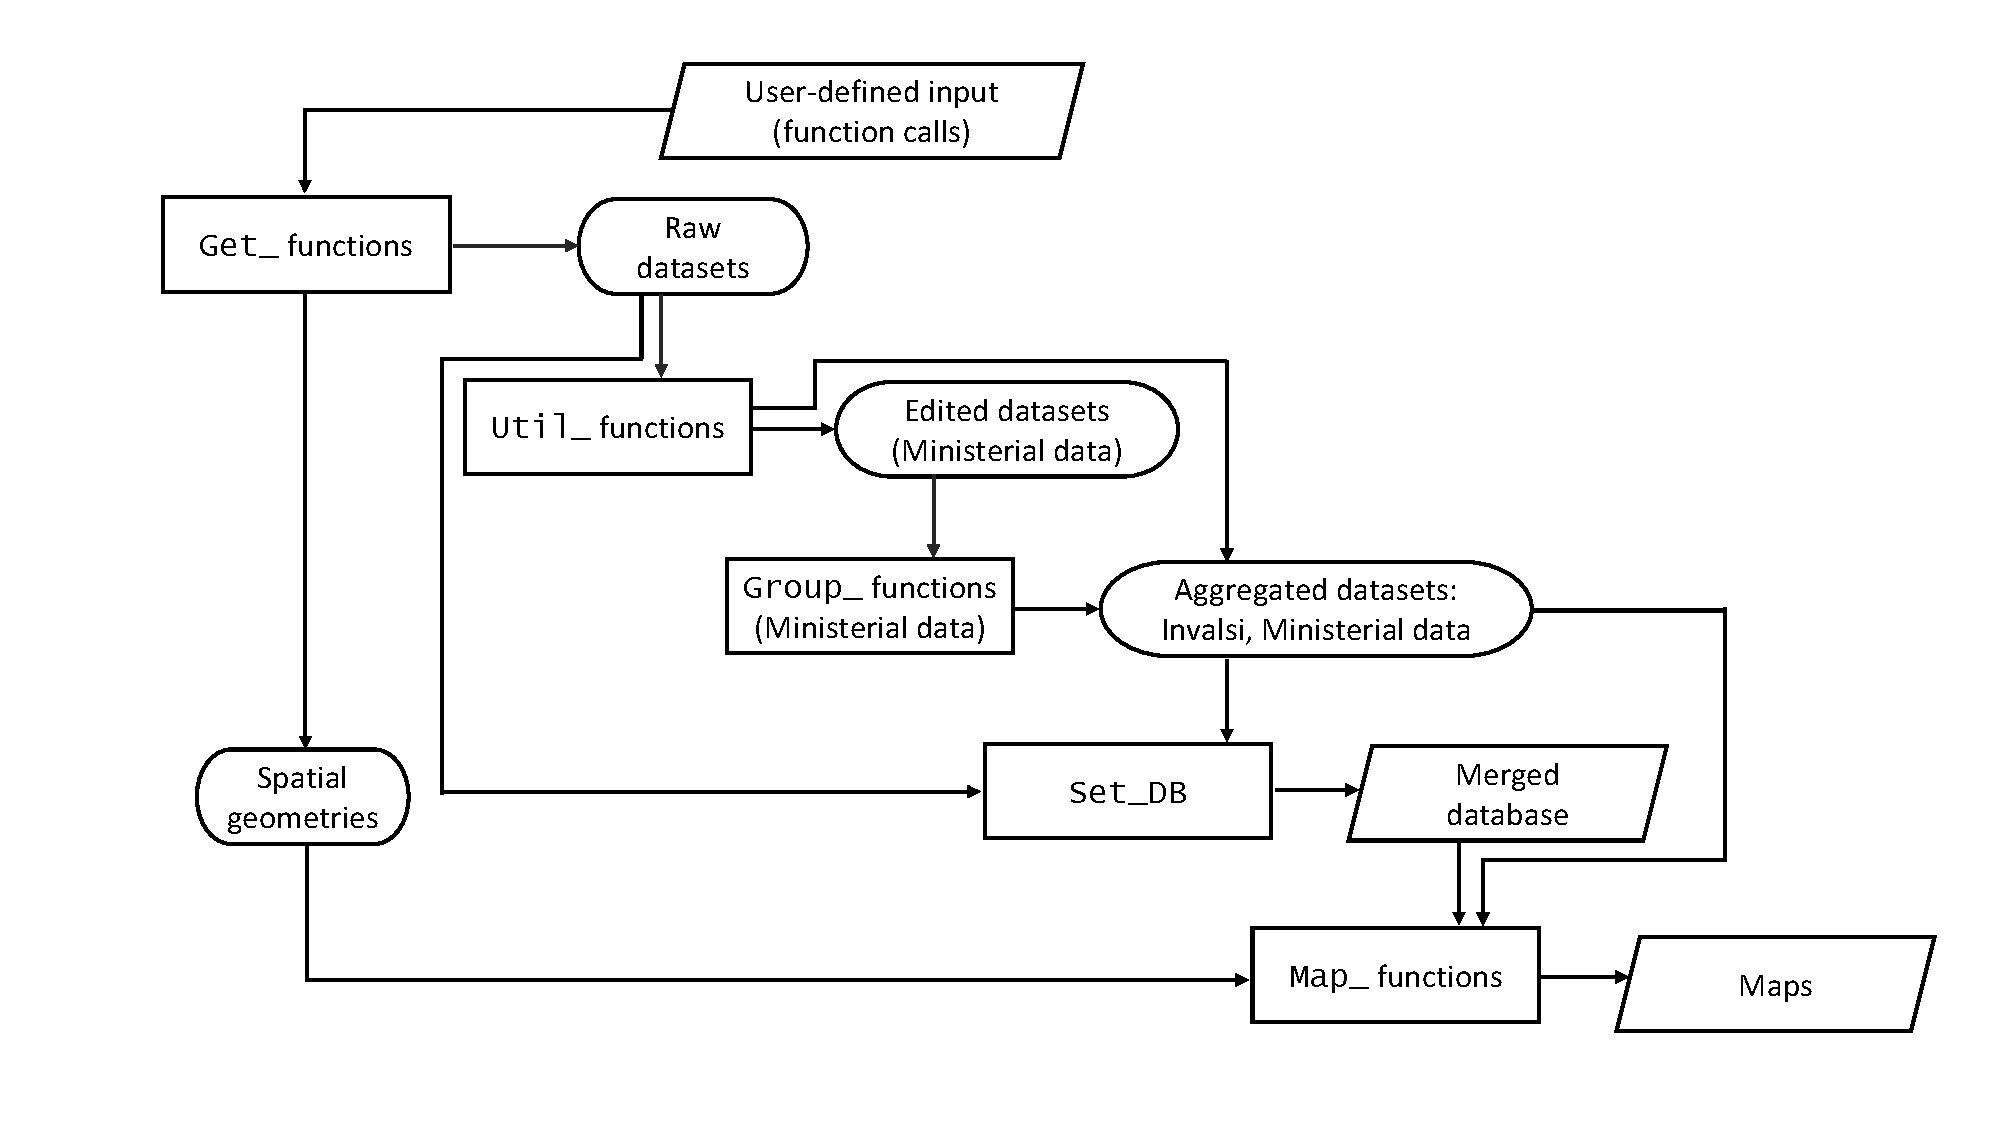
\includegraphics[width = 0.9\textwidth]{SchoolDataIT/Fig1.pdf} 
  \caption{Flowchart of the package. Rhomboids denote inputs and \texttt{R} output objects; rectangles denote functions and rounded rectangles denote intermediate \texttt{R} objects.}
  \label{fig:Flowchart}
\end{figure}

The first step involves retrieving school system data from institutional sources through the \texttt{\detokenize{Get_}} functions. The user specifies some key requests in function calls, such as the school year of interest for school buildings or student counts data. The software can thus navigate to the webpage of the data provider, inspect its HTML structure and identify the static links to the raw data to be downloaded. Raw data are then converted to \texttt{.csv} and eventually into \texttt{R} objects. In doing so, it is needful to recall that no storage space is required on the local machine of the user. 

The main retrieval functions are the following; reported data availability is assessed on April 3rd 2025.
\begin{itemize}
    \item \texttt{\detokenize{Get_DB_MIUR}} for school infrastructure data, available for school years 2015/16, 2017/18, 2018/19, 2020/21, 2021/22 and 2022/23;
    \item \texttt{\detokenize{Get_Invalsi_IS}} for Invalsi census data, available for school years from 2012/13 to 2023/24 except for 2019/2020; 
    \item \texttt{\detokenize{Get_nstud}} for student counts, available for school years 2015/16, 2017/18, 2018/19, 2020/21, 2021/22, 2022/23 and 2023/24;
    \item \texttt{\detokenize{Get_BroadBand}} for the activation status of the ultra-broadband connection across single schools at a user-specified date;
    \item \texttt{\detokenize{Get_nteachers_prov}} for teachers counts by province, available for the same school years as the school buildings data;
    \item \texttt{\detokenize{Get_Registry}} for the National Schools Registry, available for school years from 2015/16 to 2024/25;
    \item \texttt{\detokenize{Get_School2mun}} to map each school to the relevant administrative unit codes, available for the same years as the school buildings data.
\end{itemize}
The resulting objects are faithful to the original data published by providers, since at this stage data are not edited yet besides some manual corrections to municipality and province names needed for harmonising and mapping. 

Indeed, data manipulation is reserved for the subsequent step, namely the \texttt{\detokenize{Util_}} functions. One aim of these auxiliary functions is to transform input data into objects that can be handled with the next group of functions. The other aim is to perform data quality checks or editing. This group includes \texttt{\detokenize{Util_Check_nstud_availability}} to check how many schools have available the student counts, \texttt{\detokenize{Util_DB_MIUR_num}} to structure Boolean and numeric fields in the school buildings database or remove either observations with missing fields or fields with a given amount of missing observations, \texttt{\detokenize{Util_Invalsi_filter}} to filter the Invalsi survey for the school year, grade and subject, and \texttt{\detokenize{Util_nstud_wide}} to reshape the student counts dataset for it to have one school per row, compute average classroom size for each school grade, and filter out schools for which the classroom size is considered an outlier. Additional details on these functions are provided in Section \ref{section:Data}. 

Ministerial data are provided at the school level. \texttt{\detokenize{Group_}} functions allow users to bring them to the same level of detail, namely at the LAU or NUTS-3 level. 
The function \texttt{\detokenize{Set_DB}} merges one or more datasets from any previous step into a unique, aggregated database which can be considered as the final data output of the package workflow.

Lastly, the \texttt{\detokenize{Map_}} functions render aggregated data with static or dynamic choropleth maps. Notice that the former employs the \texttt{ggplot2} \citep{ggplot} environment for graphical representation, allowing a simplified export. Interactive maps, obtained through the \texttt{leaflet} \citep{leaflet} and \texttt{mapview} \citep{mapview} libraries, preserve all the information of the dataset to be rendered. Spatial geometries used for mapping are provided by the Italian Institute of Statistics through specific shape files \citep{Shapefiles}.

 

%% -------- Data ---------------------------------------- %%
\section{The Italian Education System Data} \label{section:Data}
This section describes the main datasets currently retrieved and handled by the package. For the school infrastructure system evaluation, the most valuable public source of information is the Unique School Data Portal \citep{MIUR}, an open data portal managed by the Italian Ministry of Education according to Law 107/2015 \citep{law2}. The National Schools Registry (Section \ref{par:registry}), the school buildings database (\ref{par:buildings}) and the counts of students and teachers (\ref{par:nstud}) are all provided through this website. Another relevant aspect of school infrastructure assessment is the implementation of ultra-broadband connection, whose timeline, available through the ultra-broadband activation dashboard, provided by \cite{BB} has been included in the package as well.
Lastly, Invalsi censuary survey data \citep{Invalsi_IS} have been included to assess education quality (\ref{par:Invalsi}).

Italian schools are officially identified by a 10-digit alphanumeric code. In Fig. \ref{fig:diagram} we show an example of the identifiers (ID) hierarchy. The top node is the reference institute ID; intermediate nodes are the school institutes IDs; whereas bottom nodes are the school buildings IDs. For instance, under the same reference institute, two schools are located in the municipality of Casamassima (BA, code 72015) while five other ones are distributed across three buildings in the municipality of Acquaviva delle Fonti (BA, code 72001).
\begin{figure}
  \centering
  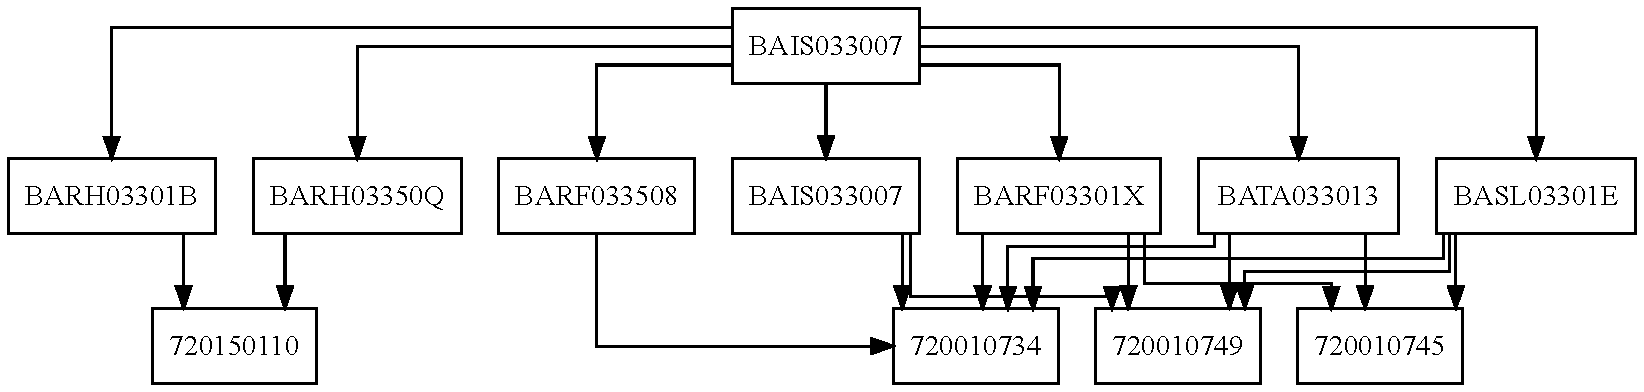
\includegraphics[width = 0.9\textwidth]{SchoolDataIT/Fig2.pdf} 
  \caption{Example of the codes of all the schools (middle nodes) and the buildings in which they are located (bottom nodes), pertaining to the same reference institute (top node)}
  \label{fig:diagram}
\end{figure}

\subsection{National Schools Registry} \label{par:registry}
The National Schools Registry includes the list of all public and private schools on the national territory. Due to the completeness of the records, this dataset is used as the baseline to harmonise other objects defined at the school level. The function \texttt{\detokenize{Get_Registry}} downloads the dataset. Notice that the relevant municipality of each school is not identified by its official administrative code but only by the cadastral code. To fill this gap, the function \texttt{\detokenize{Get_School2mun}} associates each school listed in this registry with the relevant administrative (LAU and NUTS-3) codes \citep{Situas}.

\subsection{School Buildings} \label{par:buildings}
This database covers several infrastructural dimensions, accounting for a total of about 90 variables in the last available year:
\begin{itemize}
 \item Environmental context of school buildings
 \item Accessibility through private or public transport, namely whether a building lies within a given range (e.g. 250 or 500 meters) from a transport hub
 \item Environmental or administrative restrictions 
 \item School area surface and building volume
 \item Intended use of learning and recreational spaces
 \item Overcoming architectural barriers (e.g. the presence of external ramps or stairlifts)
 \item Building and adaptation period
 \item Various information regarding heating systems
 \item Measures and devices to reduce energy consumption
 \item Acoustic insulation
 \item Static testing certification and seismic design
\end{itemize}
Observations are detailed at the level of school buildings. For this reason, the database embeds a standalone registry different from the National Schools Registry mentioned in the previous paragraph. 

The input dataset downloaded with \texttt{\detokenize{Get_DB_MIUR}} includes about $60,000$ observational units. Most variables are binary (Y/N), denoting whether a given feature occurs in a school building or not, and encoded as strings.

The function \texttt{\detokenize{Util_DB_MIUR_num}} converts strings to Boolean or numeric values when necessary. For some variables, there is a high number of missing values. For example, in school year 2022/23, the field denoting whether a school is reached by a bicycle lane is missing for $38.7\%$ of high schools, $44.1 \%$ of primary and $45.9\%$ of middle schools. The user may choose to remove either the fields with a given number of missing records ($20,000$ by default) or the units with at least one missing variable (not active by default). 

Observations can be aggregated with the function \texttt{\detokenize{Group_DB_MIUR}}. Numeric and Boolean variables are summarized by their mean and qualitative variables by their mode. Since territorial averages provide no information about missing values, by default the function returns two additional data frames providing the number of missing observations of each variable per area.

Finally, for better insight into the general infrastructural state, we add the Inner Areas taxonomy, published by the Italian Institute of Statistics (ISTAT) and updated every six years \citep{InnerAreas}. It divides Italian municipalities into six classes: A, B and C are considered central areas, while D, E, and F classes are labeled as "inner" (i.e. peripheral) areas. Class A identifies standalone pole municipalities, characterized by a comprehensive and self-sufficient combination of school, health, and transport infrastructure \citep{InnerAreas}; class B identifies inter-municipality poles, i.e. clusters of neighbouring municipalities which, taken together, fulfill the requirements of pole municipalities. The remaining classes are defined based on increasing road travel time to the closest pole: Class C: $0' - 27'42''$; Class D: $27'42'' - 40'54''$; Class E: $40'54'' - 1h \, 6' 54''$; Class F: $> 1h \, 6' 54''$.

In Figure \ref{fig:TPU23} we show the percentage of schools served by public transport in 2022/23 at the province and municipality level, in this latter case only for the Apulia region, which is the region with the highest share of municipalities hosting at least one high school ($124$ over $257$). As mentioned in Section \ref{section:Data}, though northern and central regions have a higher proportion of schools served by urban public transport, regions like Abruzzo in the South or Veneto and Emilia-Romagna in the North are in contrast the general trend. In the provinces of Aosta, Trieste, La Spezia (North), Massa (Center) and Chieti (South) all schools are reached by public transport, while this percentage is higher than $95\%$ in the provinces of Pavia, Bergamo (North), Pesaro-Urbino, Pisa, Lucca and Latina (Center). On the other hand, in the province of Salerno in Southern Italy only $0.07\%$ of schools is served by public transport; this percentage is lower than $40\%$ in the provinces of Ferrara and Pordenone in the North and Crotone, Foggia and Naples in the South.%The negative record belongs to the provinces of Salerno and Naples in Campania and Crotone in Calabria.

The code to download the raw input dataset and display these maps and all the following ones is in the Supplementary Material. 

\begin{figure}
  \centering
  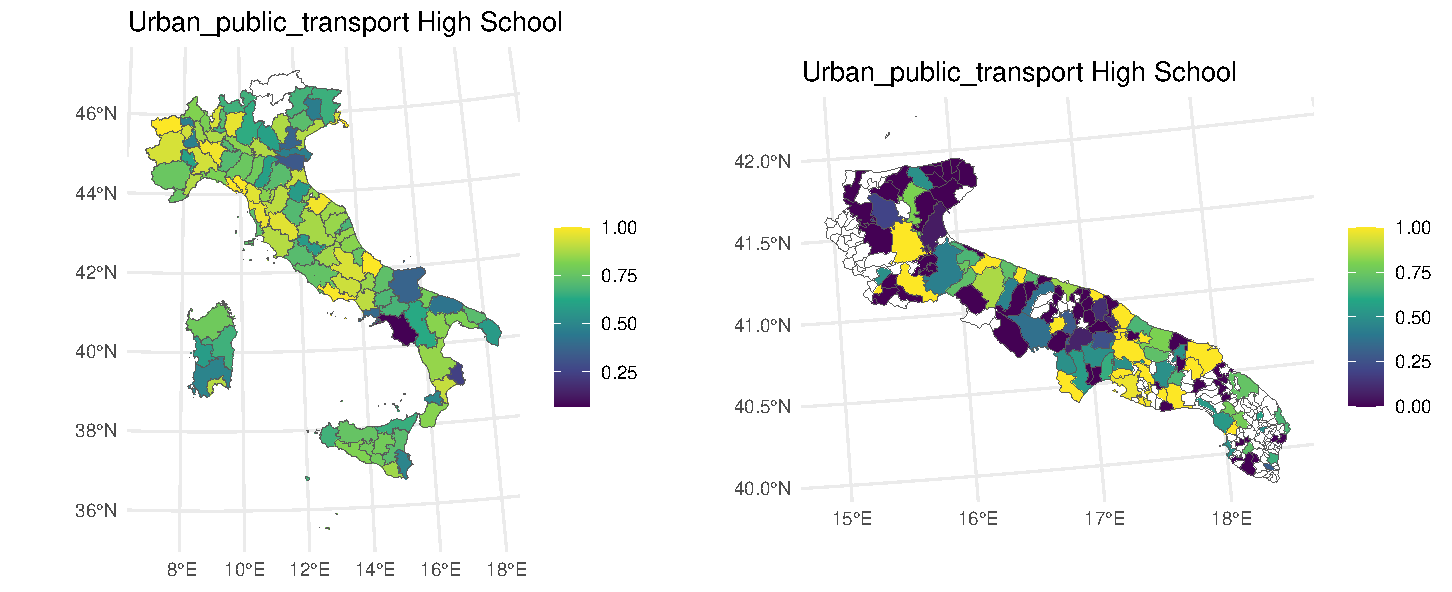
\includegraphics[width = 0.9\textwidth]{SchoolDataIT/Fig3.pdf}  
  \caption{Province-level and municipality-level percentage of high schools served by public transport in 2022/23, on the whole national territory and in the Apulia region respectively. Data of the Trentino-Alto Adige region are not provided by the Ministry.}
  \label{fig:TPU23}
\end{figure}

\subsection{Number of students and teachers} \label{par:nstud}
The Ministry of Education also publishes the counts of students per school grade for every school on the Italian territory and the counts of teachers for every Italian province. These datasets have the same temporal dimension as the school buildings database. classroom size is indeed useful information in the assessment of education quality, which is typically acknowledged to improve as classroom size decreases \citep{Blatchford, Bruhwiler}. In the case of Italy, however, caution is needed when studying the relationship between classroom size and student outcomes at the aggregate level \citep{Angrist}. In our view, an important factor to consider is how classroom size reflects the degree of centrality of municipalities. As it can be seen in Figure \ref{fig:nstud_bp_8} as an example for the last year of middle schools, peripheral areas, usually characterized by lower student outcomes, have less crowded classrooms. We will have a deeper look at the association between classroom size and education quality in Section \ref{section:Example}.
\begin{figure}
  \centering
  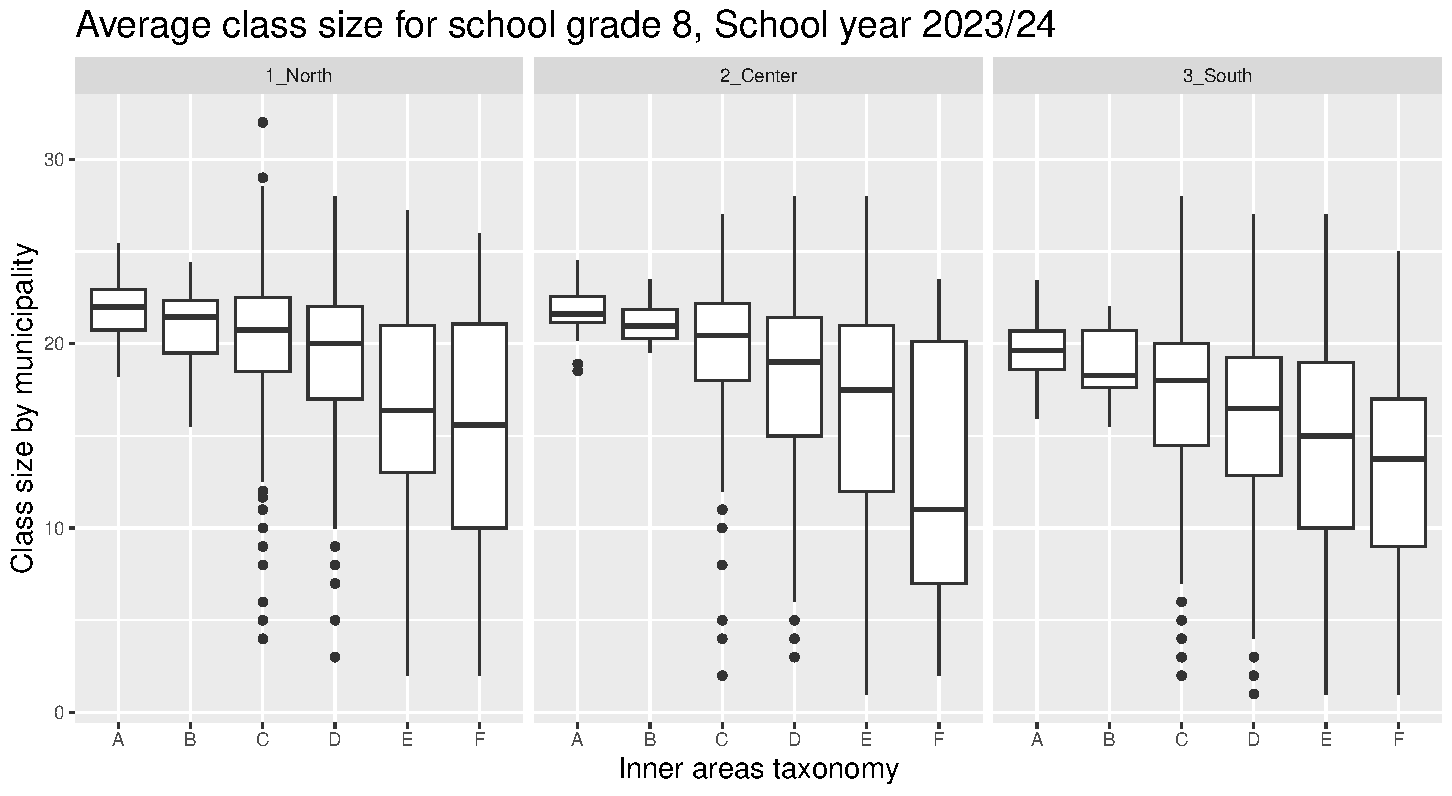
\includegraphics[width = 0.9\textwidth]{SchoolDataIT/Fig4.pdf} 
  \caption{Average municipality-level classroom size by Inner Areas taxonomy in 2023/24, last grade of middle schools. Inner area taxonomy follows a descending order of centrality: A - standalone infrastructural poles; B - inter-municipality infrastructural poles; C - belt municipalities; D - intermediate areas; E - peripheral; F - ultra-peripheral.}
  \label{fig:nstud_bp_8}
\end{figure}


The function \texttt{\detokenize{Util_nstud_wide}} rearranges the input dataset into a wide format in which each row corresponds to a school and computes the average classroom size per school for each educational grade. National regulation sets upper classroom size limits of $25$, $26$ or $27$ students in primary, middle and high schools respectively \citep[][Art. 5]{DMIM90} other than lower limits of $15$ students (8 for multi-year classes) in primary schools and $18$ students in middle schools through the Decree n.90/2023 of the Ministry of Education \citep[][Artt 10, 11]{DPR81}. A framework of waivers is established by the Ministry Decree n.90/2023 \citep{DPR81}, regarding cases of low Economic, Social and Cultural Status (ESCS) scores, high school withdrawal rate or high depopulation. 
However, the range of observed classroom sizes is often wider than the general rule, especially in high schools. In the latter case, taking the school year 2022/23 as an example, the number of schools with classroom size $\geq 40$ students was equal to $9$, $8$, $8$, $18$ and $1$ for the five high school grades respectively, over a total of $6455$ schools.
To remove values considered extreme, the user can set an upper and a lower boundary of acceptance in terms of classroom size either at the level of whole schools or single school grades. In the former case, only schools whose average classroom size (computed across all grades, e.g. for middle schools the average of 6th, 7th and 8th grades) exceeds the acceptance boundary are removed from the dataset, while in the latter case removal applies to all schools where classroom size exceeds the boundary in any grade.
For what concerns primary schools, it is also possible to download student counts by type of schooling time, namely distinguishing between full-time and half-time (only morning) schooling.

To monitor statistical data quality, the function \texttt{\detokenize{Util_nstud_check}} computes, for all municipalities and provinces, the percentage of schools listed in the National Registry for which the count of students is available. 

The function to aggregate school-level data is \texttt{\detokenize{Group_nstud}}.

Teacher counts, instead, are only available at the province level. The average number of teachers per student and per class can be computed with the function \texttt{\detokenize{Group_nteachers4stud}}. In Figure \ref{fig:nstud23} we render the average classroom size in the 2nd year of high school and the average number of teachers by student in the year 2022/2023. classroom size is higher in densely populated areas, such as the Po Valley and the surroundings of Rome and Naples, while it is smaller in most of the South, especially in the Apennines and in Sardinia. The teacher/student ratio follows a similar distribution.

\begin{figure}
  \centering
  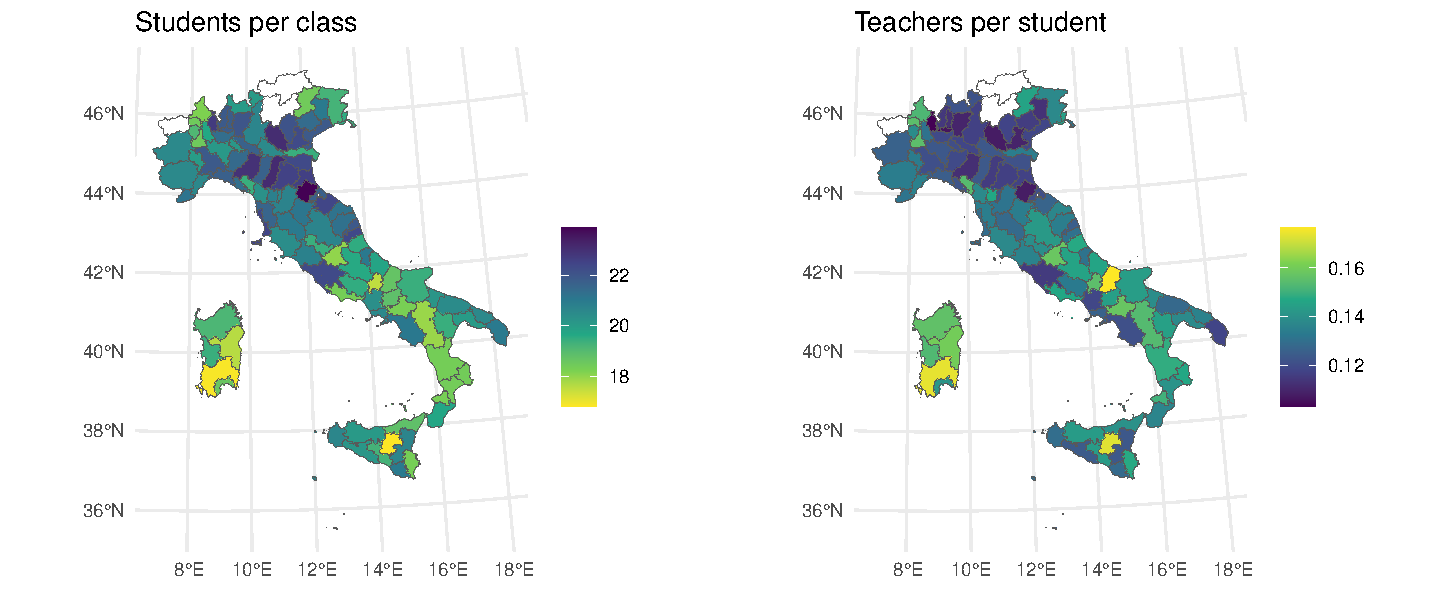
\includegraphics[width = 0.9\textwidth]{SchoolDataIT/Fig5.pdf} 
  \caption{Average province-level classroom size in the 2nd year of high school and province-level teachers/students ratio in high schools in 2022/23. Data are not available for the Trentino-Alto Adige and Aosta Valley regions. Additionally, schools with average classroom size of less than $10$ or more than $40$ students in any grade have been filtered out. }
  \label{fig:nstud23}
\end{figure}

\subsection{Ultra - Broadband connection in schools} \label{par:BB}
This dataset consists of the list of schools of the National Ultra-Broadband Plan, approved by the Ministry of Economic Development with the decree of 07/07/2020 \citep{DMise}. The Plan aims at providing 32.164 schools with internet connection with a maximum speed of 1 gigabit/second and a symmetric minimum guaranteed speed of 100 megabits/second until the peering is reached. Data are updated monthly \citep{BB}. In Table \ref{tab:broadband} in the \ref{Appendix1} we show the number of schools in which the ultra-broadband was activated in different years for all regions (one school in Trentino Alto Adige had a broadband connection before 2020). The function to download this dataset is \texttt{\detokenize{Get_BroadBand}}; the \texttt{Date} argument specifies the reference date for checking whether the ultra-broadband connection was activated or not in each school. 

\subsection{Invalsi census survey} \label{par:Invalsi}
To develop a spatially homogeneous indicator of education quality, Italian law No. 176/2007 \citep{InvalsiLaw} mandates the Italian Institute for the Evaluation of the Education System (INValSi) to assess the skills of students through a specific test. The test currently covers four subjects, Italian, Mathematics, English reading, and English listening, and is carried out yearly in the 2nd, 5th, 8th, 10th, and 13th school grades. 
The Invalsi Institute publishes several open datasets \citep{Invalsi_IS}, the widest class being that of sample surveys, which also includes anonymized microdata regarding single students. The other class of datasets consists of census surveys, detailed at either municipalities or provinces. Regarding municipality data, for privacy reasons only the municipalities with at least two schools of the same order are included in the survey; otherwise identifying average Invalsi scores of single schools would be easily possible. In this package, we focus on the census dataset since it provides more spatial information (sample datasets providing no territorial information other than the region) and is, in our judgment, more suitable for spatial analysis.  

Consistently with OECD standards \citep{PISA} the score is expressed through the weighted likelihood estimator (WLE) of student ability defined by a Rasch psychometric model, whose basic idea is that the probability that a generic student $i$ provides the correct answer to a generic item (test question) $j$ depends on two variables, namely the student ability $b_i$ and the item difficulty $d_j$. The relationship can be expressed as
$$
\mathrm{Prob} \lbrace \text{student } i \text{ answers correctly item } j \rbrace= \frac{e^{b_i - d_j}}{1 + e^{b_i - d_j}}
$$
For interpretational reasons, the estimator of $b_j$ is scaled to a global mean of 200 points and a global between-students standard deviation of 40 points. The advantage of this model is isolating the ability of students from the intrinsic difficulty of items. For primary schools only, the percentage of sufficient tests is also reported. Scores are already corrected from the effect of cheating, which would otherwise hinder their meaning, other than shrinking their variance. The functions to download and filter the Invalsi database per school year, grade and subject are respectively \texttt{\detokenize{Get_Invalsi_IS}} and \texttt{\detokenize{Util_Invalsi_filter}}. No data quality checks are deemed necessary as this dataset is already carefully processed by the Invalsi Institute.



%As an example, in Figure \ref{fig:InvalsiProv} we plot the Invalsi scores in Italian and English reading for the last year of high school at the province level in 2023/24. The North-South divide is obvious. A particularly vulnerable profile can be noticed across the provinces of Naples and Salerno (Campania) and most of the provinces belonging to Calabria, Sicily, and Sardinia (with the partial exception of the province of Cagliari). Highest scores in both subjects are observed in the provinces of Lecco, Como and Bergamo in Lombardy other than Trieste and Bolzano with respect to English scores.

%\begin{figure}
%  \centering
%  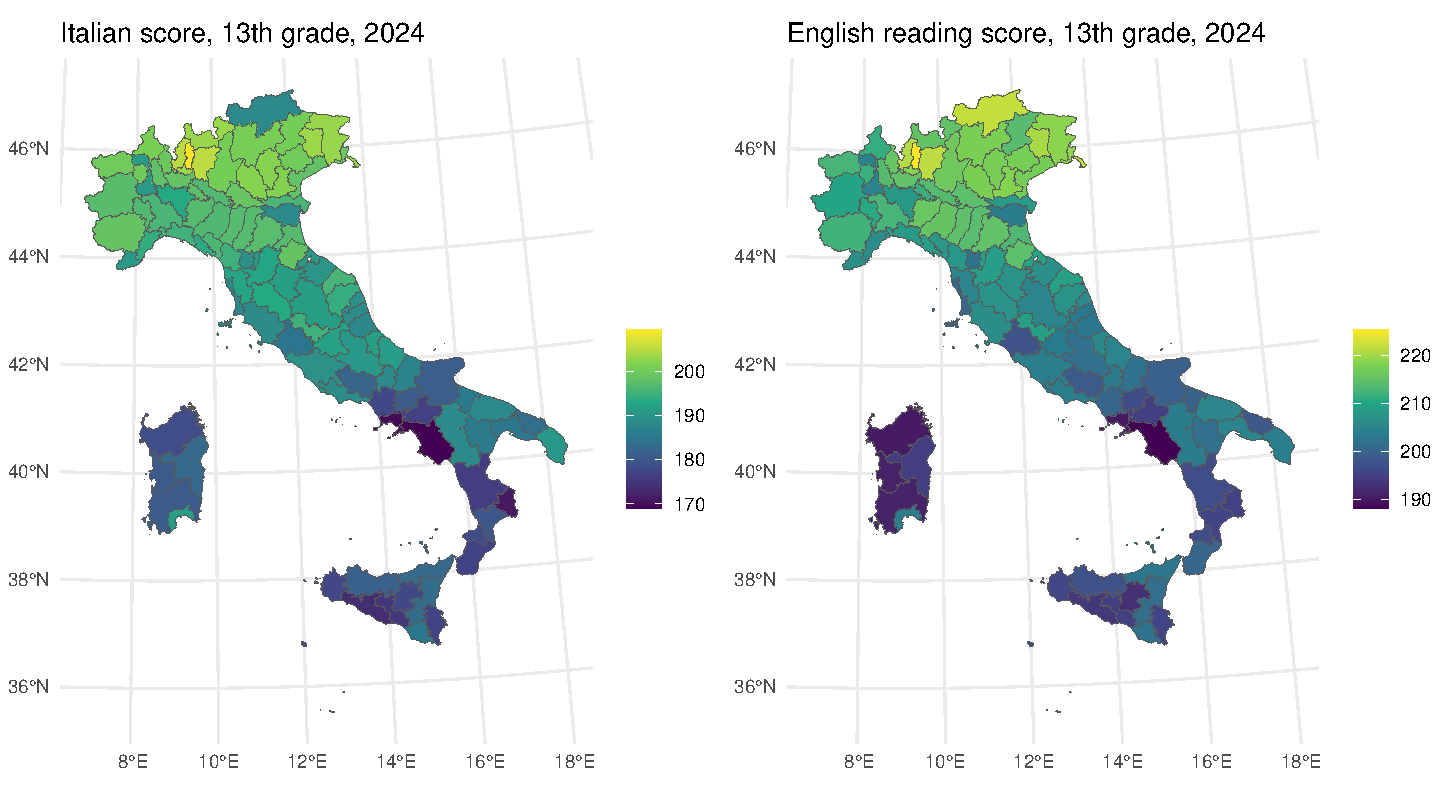
\includegraphics[width = 0.9\textwidth]{SchoolDataIT/Fig6.pdf} 
%  \caption{Invalsi scores in Italian and English reading, last year of high school, school year 2023/24}
%  \label{fig:InvalsiProv}
%\end{figure}





%% -------- Example ------------------------------------- %%
\section[Usage Example]{Student outcomes in Mathematics and classroom size: an example using the SchoolDataIT package} \label{section:Example}

Here we provide an example of spatial statistical application to the data covered by the \texttt{SchoolDataIT} package. Following Section \ref{par:nstud}, suppose the user is interested in studying to what extent classroom size is associated with student outcomes. We can first map the two variables.
%
\begin{figure}
  \centering
  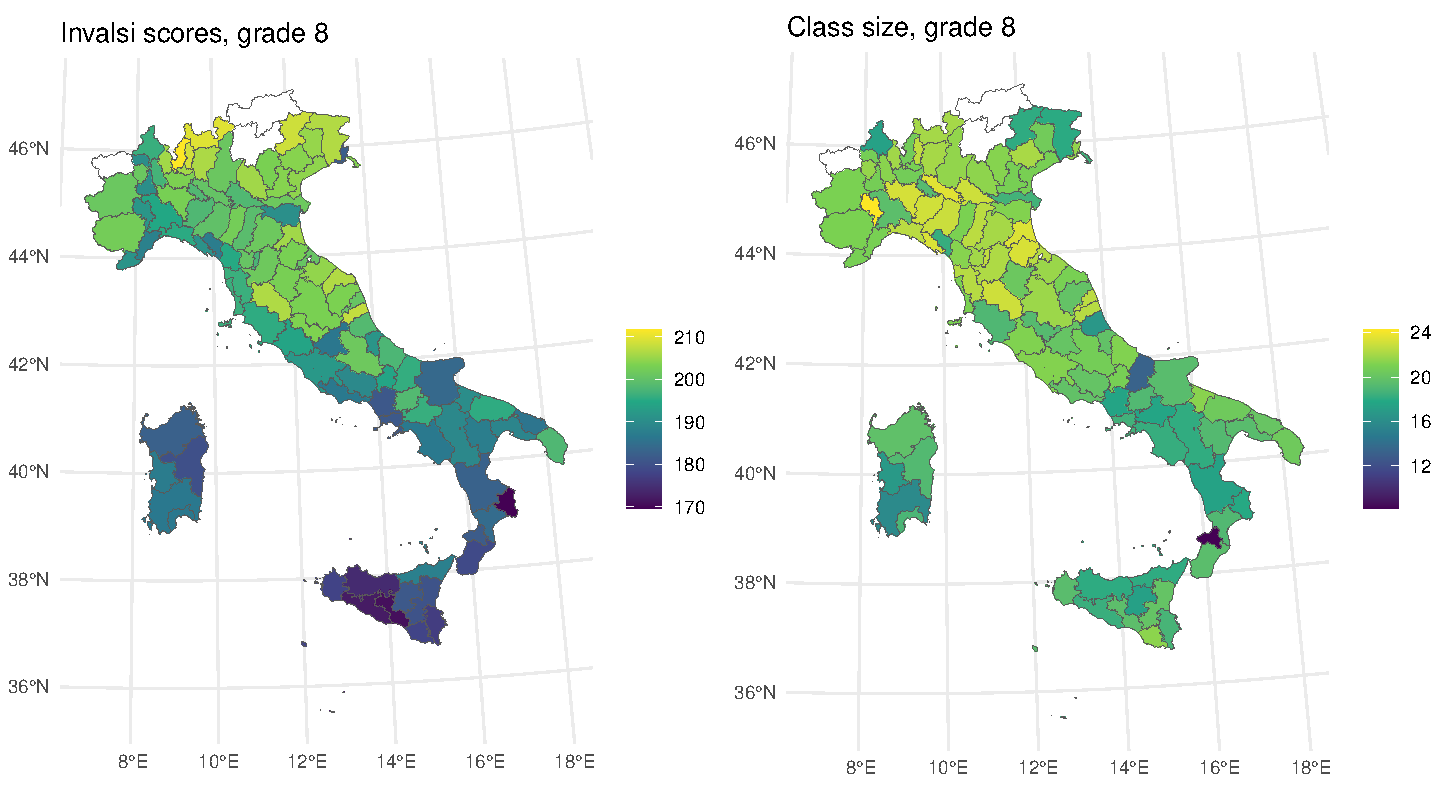
\includegraphics[width = 0.9\textwidth]{SchoolDataIT/Fig7.pdf} 
  \caption{Invalsi score in Mathematics and average classroom size, last year of middle school, school year 2023/24. Trentino-Alto Adige and Aosta Valley are not included due to lack of classroom size data.}
  \label{fig:invalsi_nstud8}
\end{figure}
%
Concerning the last year of middle school in 2023/2024, we regress the Invalsi score in Mathematics on the average classroom size at the municipality level. To ease model results interpretation, classroom size is scaled to zero mean and unit variance. Additionally, schools with an average class size of less than $10$ or more than $40$ students have been removed from the dataset. 
In this case, observational length is equal to $n = 780$ municipalities, i.e. those for which Invalsi scores and classroom size were both available at 2025/04/03.

OLS regression would result in an expected effect of classroom size equal to $4.153$, with standard error $0.407$. If no additional information is taken into account, classroom size would then appear to have a positive and statistically significant relationship with Invalsi scores.
%Under the OLS specification, the stochastic representation of the Invalsi score, which we denote as $y$, is
%\begin{equation}
%y = \beta_0 +  \beta_\mathrm{nstud} X_\mathrm{nstud} + \varepsilon
%\label{eq:OLS}
%\end{equation}

%where $\beta_0$ is the intercept, $X_\mathrm{nstud}$ is classroom size, $\beta_\mathrm{nstud}$ is the effect of classroom size, and $\varepsilon$ is a Gaussian IID error such that $\varepsilon \sim N  (0, \sigma_{\varepsilon}^2 I_n)$. 

%If no additional information is taken into account, classroom size appears to have a positive and statistically significant association with the Invalsi score, as seen in \ref{tab:OLS}:
%
% \begin{table}
% \centering
%\begin{tabular}{lrrrr}
% & mean & s.d. & $Q_{0.025}$ & $Q_{0.975}$ \\
% \hline
% $\beta_0$ (intercept)& 194.551 & 0.406 & 193.755 & 195.347 \\ 
% $\beta_{nstud}$ & 4.153 & 0.407 & 3.356 & 4.951 \\ 
% \hline
%\end{tabular}
%\caption{Effect of classroom size on Invalsi scores in Mathematics in the last year %of middle school, using the model in eq. \ref{eq:OLS}}
%\label{tab:OLS}
%\end{table}
%
A closely linked result, namely the significantly positive association of Invalsi scores with the students/teacher ratio, was noticed by \cite{Barbieri}, always in the context of middle schools, and attributed to the impact of schools reputation on their attractiveness. Interestingly, when an instrumental variable relating to teachers' mobility was taken into account in their regression model, the estimated effect of the student-to-teacher ratio was not significant anymore.

Given the greater amount of information at our disposal, it would be na{\"i}ve to limit the analysis to this amount of information. First, considering what we have seen in \ref{fig:nstud_bp_8}, the user may be interested in adding the inner areas taxonomy as an explanatory variable in the simplest possible way, namely classifying municipalities among central (A, B, C) and inner (C, D, E) areas. Moreover, the territorial structure of the dataset suggests to include spatial terms in the regression model. Considering the number of municipalities for which data are available ($780$ over a national total of $7901$), the spatial structure is rather sparse and we would need to define some neighbouring rules in alternative to shared borders. To overcome this issue, we choose to treat the municipality-level average Invalsi score as a point-referenced process, thus assuming that the data-generating process is defined on a continuous spatial domain. Specifically, we postulate that the locations at which this process is observed are the centroids of municipalities as defined on January 1st, 2023.
Spatial information is taken into account through a linear spatial trend and a spatially structured Gaussian process $u(s)$, with $s \in [1, 780]$, whose autocorrelation decays as distance increases. The model becomes thus:
%
\begin{equation}
y(s) = \beta_0 + \beta_\mathrm{nstud} X_\mathrm{nstud}(s) + \beta_{I} X_{I}(s) + \beta_{\ell} \ell(s) +\beta_{\phi} \phi(s) + u(s) + \varepsilon(s)
\label{eq:spde}
\end{equation}
%
where $\beta_0$ is the intercept, $X_\mathrm{nstud}$ is classroom size, $X_I$ is the dummy for the inner areas taxonomy ($1$: inner area, $0$: central area), $\ell$ is the longitude of municipality centroids, $\phi$ is the latitude; $\beta$ terms are covariates effects; $\varepsilon$ is a Gaussian IID error such that $\varepsilon \sim N  (0, \sigma_{\varepsilon}^2 I_n)$. $u$ follows \textit{a priori} a Normal distribution with mean zero and covariance matrix whose elements depend on the distance between the two corresponding points, but not on the direction of their link (isotropy); second-order stationarity is additionally assumed for $u$ \citep[][ Section 2.1]{Banerjee}. Based on these two assumptions, we assign $u$ the Matérn covariance function, which depends on a global variance $\sigma^2$ and a range parameter $r$. In detail, the Matérn covariance function between two generic sites $i$ and $j$ is given by:

%
\begin{equation}
\sigma_{ij} =\sigma^2 \frac{1}{2^{\nu-1}\Gamma(\nu)} \left(\kappa  d_{ij}\right)^{\nu}
K_{\nu}(\kappa d_{ij}) 
\label{eq:matern}
\end{equation}
%


where $d_{ij}$ is the Euclidean distance between the $i$-th and $j$-th location, $\sigma^2$ is the global (common across locations) variance, %$\tau_0$ is the inverse nugget effect;
$\kappa$ is a scale parameter and $\nu$ controls smoothness. These parameters are linked to the range $r$ since in this model $r = \frac{\sqrt{8\nu}}{\kappa}$. In this example, we keep fixed $\nu = 1$.  $K_{\nu}(x)$ denotes the modified Bessel function of the second kind \citep[][Section 9.6]{AS}:

$$
K_{\nu}(x) = \frac{\pi \left( I_{-\nu}(x) - I_{\nu}(x)\right)}{2 sin (\nu \pi)}
$$

Where $I_{\nu}(x)$ denotes the modified Bessel function of the first kind, defined in turn as a solution to the equation $I_\nu(x) = f:x^2 + \frac{d^2f(x)}{dx^2}+x\frac{df(x)}{dx} - (x^2+\nu^2)f(x) = 0$:

$$
I_{\nu}(x) = \sum_{k=0}^\infty \left( \frac{x}{2} \right)^{2k+\nu}\frac{1}{k! \Gamma(k+\nu+1)}
$$

Now, \cite{Whittle} shown that a stochastic process $u(s)$ with this kind of covariance function is a solution to the SPDE (we limit our illustration to the bidimensional case):

\begin{equation}
(\kappa^2 - \Delta)^{\frac{\nu + 1}{2}} \tau u(s) = \epsilon(s)
\label{spde}
\end{equation}

Where $\Delta$ is the Laplacian operator and $\epsilon(s)$ denotes a spatial Gaussian white noise process; this equation \textcolor{red}{does describe indeed a Gaussian autoregressive process on an infinite lattice}.

Parameters $\nu$ and with $\kappa$ are linked to the global variance $\sigma^2$ through the relationship:
$$
\sigma^2 = \frac{\Gamma(\nu)}{\Gamma(\nu +1) 4 \pi \kappa^{2 \nu} \tau^2}
$$


Fitting spatial models such as the one in equation \ref{eq:spde} implies the inversion of the covariance matrix of $u$, which is typically dense as it can be seen from equation \ref{eq:matern}. In geostatistical literature, this issue is typically referred to as the big-$n$ problem \citep{bigN} as the inversion operation has a computational cost in $\mathcal{O}(n^3)$. 

A potential solution is offered by the Stochastic Partial Differential Equation (SPDE) approach for Gaussian fields. \cite{SPDE} show, indeed, that processes with Matérn covariance function can be represented as Gaussian Markov Random Fields defined on a discrete spatial domain, which is determined via Delaunay triangulation over a manifold technically known as mesh. 

The point-referenced field $u(s)$ is replaced by $A z$ where $A$ is an $n \times N$ matrix to project observation locations onto the mesh, and $z$ is a Gaussian Markov random field of length $N$ defined on the mesh which, in our case, has $N = 1384$ nodes. Markov properties, together with the Normal distribution, ensure the precision matrix of $z$ has a number of nonzero entries in the order of $N$ \citep{GMRFs}, as seen in Section \ref{section:GMRFs}. 

Mapping the Matérn field onto a GMRF shrinks the computational cost to $\vartheta(N^{3/2})$. \textcolor{red}{TBD: AGGIUNGERE FONTE O DIMOSTRARE}


For model fitting, we firstly need to define the mesh and index all its nodes; in our case the mesh is chosen to have more nodes than the observation points. This procedure can be entirely handled internally to \texttt{R-INLA}.

%The object \texttt{A.mat} is the projection matrix $A$. We are fitting a hierarchical Bayesian model, requiring prior assumptions on the distribution of all parameters of interest and on hyper-parameters as well. Firstly, we define a PC-prior on the range $r$ and the global standard deviation $\sigma$ of the random effect. The behaviour of these distribution is described in \cite{SPDEPC}. In brief, we select two fixed hyper-parameters, $\sigma_0$ and $r_0$ such that, for two fixed values $p_\sigma$ and $p_r$, it holds that:
%$$
%\left\{\begin{array}{ll}
%prob \left( r < r_0 \right) = p_r \\
%prob \left( \sigma > \sigma_0 \right) = p_\sigma
%\end{array} \right.
%$$
%Based on prior knowledge and ignoring information available from explorative data analysis, we are assuming here that the range, namely the distance at which the correlation of the random fields is shrunk under a $0.10$ threshold is smaller than $400$ kilometers with $95\%$ probability, and at the same probability the standard deviation of the random field exceeds $6$ points.


The hierarchical model in equation \ref{eq:spde} also requires prior assumptions on the distribution of its hyperparameters. Error precision $\sigma_{\varepsilon}^{-2}$ is assumed to follow a Gamma distribution with shape parameter $1$ and rate parameter $ 5 \cdot 10^{-5}$. Moreover, we define a penalized complexity (PC) prior \citep{PC} on the range $r$ and the global standard deviation $\sigma$ of the latent spatial field. The behaviour of these distributions is described in \cite{SPDEPC}. We select two fixed values, $\sigma_0$ and $r_0$ such that, for two fixed values $p_\sigma$ and $p_r$, $prob \left( r < r_0 \right) = p_r $ and $prob \left( \sigma > \sigma_0 \right) = p_\sigma$. 

Based on prior knowledge and ignoring the information available from exploratory data analysis, we assume that the range, namely the distance at which the correlation of the random fields is shrunk under a $0.10$ threshold, is smaller than $300$ kilometers with $5\%$ probability, and the standard deviation of the random field is higher than $4$ points with $5\%$ probability. Again, for the sake of model results interpretation, classroom size, latitude and longitude are scaled to mean $0$ and variance $1$. 

 

%In brief, considering a hierarchical model setting in which the distribution of the parameters of interest depends on a second layer of parameters, namely the hyperparameters,the INLA approximates the posterior distribution of hyperparameters by Laplace approximation \citep{INLA}. The posterior distribution of the parameters is obtained subsequently by marginalizing hyperparameters out of the approximated full conditional, which in turn undergoes a Variational Bayes correction to the mean \citep{INLAVB}. Discussing thoroughly how to make inferences by applying the INLA to Matérn fields lies beyond the scope of this paper. A complete overview of the treatment for these models can be found in \cite{INLASPDE}.



The summaries of covariate effects are reported in Table \ref{tab:betaSP}.
%
 \begin{table}
 \centering
\begin{tabular}{lrrrr}
 & mean & s.d. & $Q_{0.025}$ & $Q_{0.975}$ \\
 \hline
 $\beta_0$ (Intercept) & 195.103 & 1.080 & 192.918 & 197.211 \\  
 $\beta_{nstud}$ 0.192 & 0.317 & -0.429 & 0.813 \\ 
 $\beta_I$ & -2.329 & 0.719 & -3.743 & -0.920 \\ 
 $\beta_{\phi}$ & 8.997 & 1.044 & 6.928 & 11.061 \\ 
 $\beta_{\ell}$ &  1.865 & 1.038 & -0.174 & 3.934 \\ 
 \hline
\end{tabular}
\caption{Estimated effects of classroom size, inner area dummy, latitude and longitude on Invalsi scores in Italian, last year of middle school, under model \ref{eq:spde}}
\label{tab:betaSP}
\end{table}
%
Employing this amount of information, the effect of classroom size no longer appears to be significant, while belonging to an inner area still implies an expected disadvantage of $2.329 $ points in Invalsi scores compared to central areas (either infrastructural poles or municipalities close to them). The evidence for the North-South divide is very strong, as the current model suggests that being located one standard deviation of the northing distribution ($\approx 291.25$ km) further north than a reference location implies an expected advantage of $8.997$ Invalsi points. To visualize the extent to which the spatial structure influences Invalsi scores, we plot the expected value of the linear trend ($\beta_\ell \ell + \beta_\phi \phi$) and the latent Gaussian process ($u$) in Figure \ref{fig:trends}.

The darker zones in the right panel (lower values of $\mathbf{E}[u|y]$) can be interpreted as areas of educational vulnerability net of classroom size, general infrastructural conditions, and net of the North-South trend as well. Most critical areas include the urban area of Naples and the upper Ionian coast in Calabria. Conversely, brighter areas represent relatively advantaged territories, such as much of  Central inland and the Salento Peninsula.

\begin{figure}
  \centering
  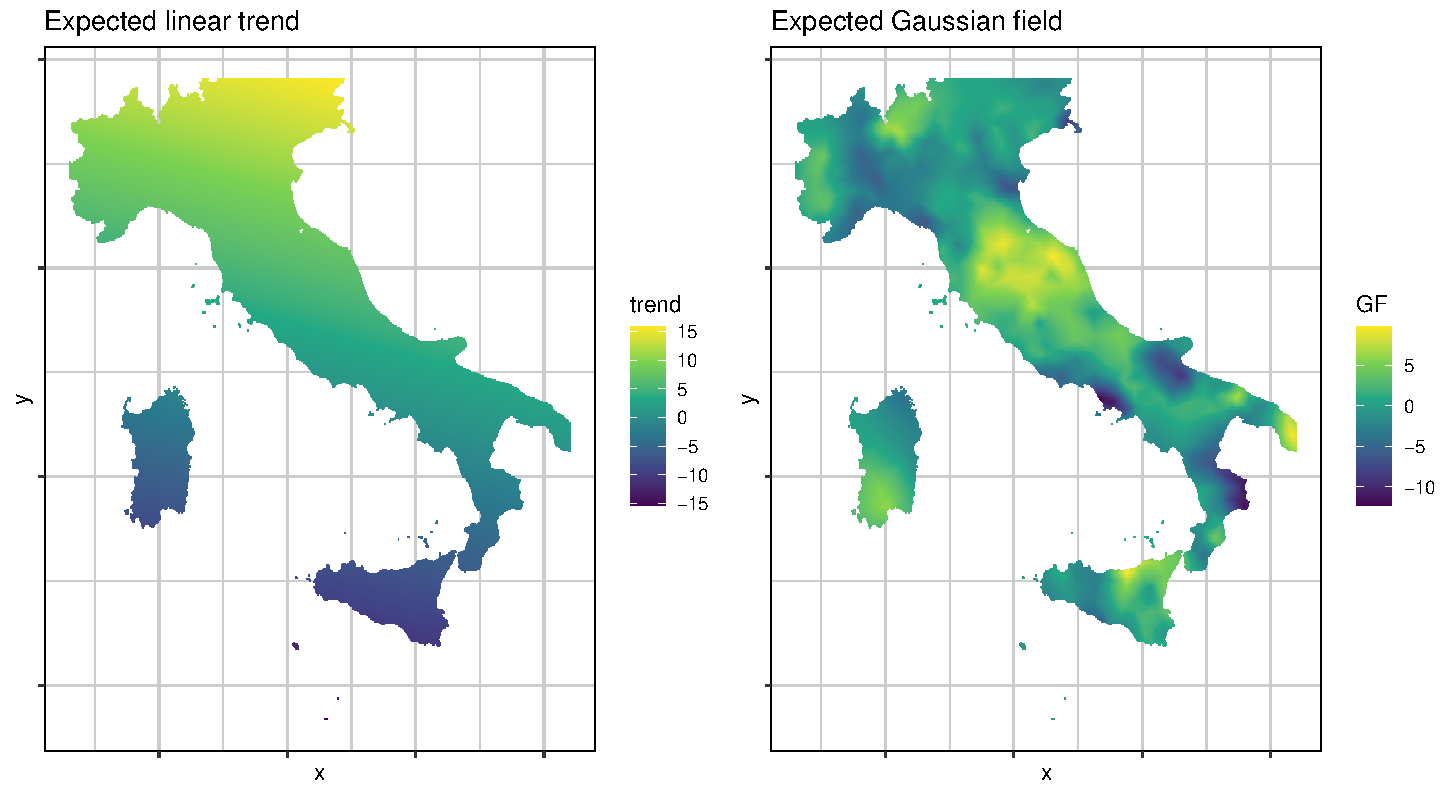
\includegraphics[width = 0.9\textwidth]{SchoolDataIT/Fig8.pdf} 
  \caption{Posterior expectation of the linear trend on the left and of the spatial latent variable on the right, the latter being added to the model to explain spatial variability in Invalsi scores after controlling for the linear trend and the explanatory variables.}
  \label{fig:trends}
\end{figure}


This simple example highlights that assessing the impact of classroom size on student outcomes is somewhat less simple than it may initially appear and warrants a multidimensional analysis. Even though only aggregated data are taken into account, auxiliary information such as the degree of centrality of a municipality or the spatial location becomes thus crucial.





%% -------- Conclusions --------------------------------- %%
\section{Concluding remarks}
The package \texttt{SchoolDataIT} allows \texttt{R} users to automatically construct an organic database by combining from different sources those open data we deem to be the most informative about the Italian education system and the state of school infrastructure in Italy, covering some of the Ministerial open data sets (e.g., the Schools Registry, the school buildings database, students and teachers counts), the Invalsi census survey, and the registry of Ultra-Broadband activation status. 

One key feature we emphasize is the relevance of the spatial context, hence territorial units of aggregated data can be easily associated either with their boundaries or centroids. With this library, we aim to provide an insight into the state of the Italian education system as clearly as possible, to ease statistical analysis on its main aspects, also employing a spatial framework, and to identify areas of education vulnerability following either a unidimensional or a multidimensional approach. With this in mind, exploratory analysis should be facilitated by mapping functions. While this paper presents a cross-sectional data usage example, panel analysis is possible as well, considering a current observation length of six years. 

Although the present version of the package covers a given amount of data, implementing any additional function to retrieve, edit and structure further data sets would not imply a significant increase in file weight for the package. Therefore, a possible line of development of this package would be to plug in additional data sets.

Lastly, the package appeals to generic \texttt{R} users, from whom the various functions are designed to require as little effort as possible. Despite our efforts for maintaining a user-friendly perspective, the final output of this package is data objects defined coherently with the \texttt{Tidyverse} environment to ensure object portability and ease of use of the present data also outside \texttt{R}.



%%%%%%%%%%%%%%%%%%%%%%%%%%%%%%%%%%%%%%%%
%%%%%%%%%%%%%%% Appendix %%%%%%%%%%%%%%%
%%%%%%%%%%%%%%%%%%%%%%%%%%%%%%%%%%%%%%%%
\newpage
%\appendix
\begin{appendices} 

 

\section{Tables} \label{Appendix1}
\begin{table}[ht]
\centering
%\begin{scriptsize}
\resizebox{\textwidth}{!}{
\begin{tabular}{lrrrrrr}
  \hline
   & \multicolumn{2}{c}{Primary}& \multicolumn{2}{c}{Middle}& \multicolumn{2}{c}{High}\\
  Seismicity & buildings & \% tot. & buildings & \% tot. & buildings & \% tot. \\ 
  \hline
  High     & 1375 & 7.53\%  & 877  & 8.45\%  & 662  & 6.1\% \\ 
  Mid-High & 6999 & 38.33\% & 3938 & 37.96\% & 4267 & 39.31\% \\ 
  Mid-Low  & 7197 & 39.42\% & 3970 & 38.27\% & 4402 & 40.55\% \\ 
  Low      & 2687 & 14.72\% & 1589 & 15.32\% & 1524 & 14.04\% \\ 
   \hline
\end{tabular}
}
%\end{scriptsize}
\caption{Seismic risk classification of municipalities hosting school buildings}
\label{tab:seismicity}
\end{table}

%%%%%%%%%%%%%%%%%%%%%%%%%%%%%%%%%%%%%%%%%%%%%%%%%%%%%%%%%%%%%%%%%%%%%%%%%%%%%%%%%




\begin{table}[ht]
\centering
%\begin{scriptsize}
\resizebox{\textwidth}{!}{
\begin{tabular}{lrrrrrr}
  \hline
   & \multicolumn{2}{c}{Primary}& \multicolumn{2}{c}{Middle}& \multicolumn{2}{c}{High}\\
  Region & buildings & \% tot. & buildings & \% tot. & buildings & \% tot. \\ 
  \hline
  Abruzzo &  87 & 19.46\% &  62 & 22.46\% &  40 & 17.24\% \\ 
  Basilicata &  99 & 39.76\% &  73 & 40.33\% &  61 & 33.7\% \\ 
  Calabria & 608 & 60.5\% & 399 & 60.73\% & 234 & 52.58\% \\ 
  Campania & 191 & 10.43\% & 140 & 13.17\% & 143 & 12.25\% \\ 
  Emilia - Romagna &   1 & 0.09\% &   1 & 0.16\% &   0 & 0\% \\ 
  Friuli - Venezia Giulia &  42 & 8.47\% &  24 & 10.04\% &  16 & 6.3\% \\ 
  Lazio &  67 & 4.87\% &  34 & 4.32\% &  28 & 3.16\% \\ 
  Liguria &   0 & 0\% &   0 & 0\% &   0 & 0\% \\ 
  Lombardia &   1 & 0.04\% &   0 & 0\% &   0 & 0\% \\ 
  Marche &   2 & 0.38\% &   2 & 0.67\% &   0 & 0\% \\ 
  Molise &  40 & 30.3\% &  23 & 25.27\% &  21 & 22.11\% \\ 
  Piedmont &   0 & 0\% &   0 & 0\% &   0 & 0\% \\ 
  Apulia &  16 & 1.65\% &  14 & 2.34\% &  11 & 1.19\% \\ 
  Sardinia &   1 & 0.16\% &   2 & 0.41\% &   0 & 0\% \\ 
  Sicily & 131 & 7.78\% &  60 & 6.47\% &  48 & 4.75\% \\ 
  Tuscany &   0 & 0\% &   0 & 0\% &   0 & 0\% \\ 
  Umbria &  52 & 14.44\% &  25 & 12.69\% &  36 & 20.11\% \\ 
  Aosta Valley &   0 & 0\% &   0 & 0\% &   0 & 0\% \\ 
  Veneto &  37 & 2.26\% &  18 & 2.05\% &  24 & 2.97\% \\ 
  
   \hline
\end{tabular}
}
%\end{scriptsize}
\caption{School buildings located in high seismicity municipalities, both in absolute numbers and as a proportion of the regional total}
\label{tab:risk1}
\end{table}



%%%%%%%%%%%%%%%%%%%%%%%%%%%%%%%%%%%%%%%%%%%%%%%%%%%%%%%%%%%%%%%%%%%%%%%%%%%%%%%%%


%\begin{table}[ht]
%\centering
%\resizebox{\textwidth}{!}{
%\begin{tabular}{llllllllll}
%  \hline
% & \multicolumn{3}{c}{Seismic design}  & \multicolumn{3}{c}{Seismic adaptation}  & \multicolumn{3}{c}{Seismic improvement} \\ 
% Region& High & Middle & Primary& High & Middle & Primary& High & Middle & Primary\\
%  \hline
%Abruzzo & 65\% & 42.11\% & 44.12\% & 32.5\% & 5.26\% & 8.82\% & 0\% & 5.26\% & 8.82\% \\ 
%  Basilicata & 23.08\% & 44.68\% & 38.1\% & 9.62\% & 6.38\% & 7.94\% & 0\% & 10.64\% & 11.11\% \\ 
%  Calabria & 47.29\% & 35.53\% & 28.87\% & 3.88\% & 34.21\% & 23.85\% & 0\% & 2.63\% & 5.86\% \\ 
%  Campania & 59.02\% & 59.18\% & 49.23\% & 0\% & 4.08\% & 4.62\% & 1.64\% & 6.12\% & 1.54\% \\ 
  % % %Emilia-Romagna &  & 100\% & 0\% &  & 0\% & 0\% &  & 100\% & 100\% \\ 
%  Friuli-Venezia Giulia & 100\% & 76.47\% & 69.7\% & 6.25\% & 5.88\% & 6.06\% & 0\% & 0\% & 0\% \\ 
%  Lazio & 24\% & 71.43\% & 29.41\% & 4\% & 0\% & 0\% & 0\% & 0\% & 0\% \\ 
  % % %Lombardia &  &  & 0\% &  &  & 0\% &  &  & 0\% \\ 
  % % %Marche &  & 100\% & 100\% &  & 0\% & 0\% &  & 0\% & 0\% \\ 
%  Molise & 26.67\% & 61.54\% & 50\% & 6.67\% & 7.69\% & 3.85\% & 6.67\% & 15.38\% & 15.38\% \\ 
%  Apulia & 28.57\% & 15.38\% & 12.5\% & 28.57\% & 15.38\% & 12.5\% & 14.29\% & 15.38\% & 18.75\% \\ 
  % % %Sardinia &  & 0\% & 0\% &  & 0\% & 0\% &  & 0\% & 0\% \\ 
%  Sicily & 42.22\% & 36.36\% & 30.19\% & 0\% & 0\% & 0\% & 0\% & 6.82\% & 3.77\% \\ 
%  Umbria & 41.67\% & 41.67\% & 44.44\% & 0\% & 0\% & 3.7\% & 8.33\% & 33.33\% & 22.22\% \\ 
%  Veneto & 20.83\% & 18.18\% & 22.22\% & 4.17\% & 9.09\% & 14.81\% & 0\% & 9.09\% & 0\% \\ 
%   \hline
%\end{tabular}
%}
%\caption{Proportion of schools in high-seismicity areas either built according to seismic design standards or subject to seismic adaptation or seismic improvements}
%\label{tab:SeismAdaptSevere}
%\end{table}

 %%%%%%%%%%%%%%%%%%%%%%%%%%%%%%%%%%%%%%%%%%%%%%%%%%%%%%%%%%%%%%%%%%%%%%%%%%%%%%%%%%%%%%%
\begin{table}[ht]
\centering
%  \begin{scriptsize}
\begin{tabular}{lrrr}
  \hline
  Region & HT Students & FT Students  & \% Full Time \\ 
  \hline
  Abruzzo & 37956 & 11796 & 23.71\% \\ 
  Basilicata & 9660 & 10275 & 51.54\% \\ 
  Calabria & 56018 & 19730 & 26.05\% \\ 
  Campania & 181001 & 47326 & 20.73\% \\ 
  Emilia - Romagna & 78588 & 95936 & 54.97\% \\ 
  Friuli - Venezia Giulia & 23497 & 19326 & 45.13\% \\ 
  Lazio & 86366 & 131766 & 60.41\% \\ 
  Liguria & 22811 & 27457 & 54.62\% \\ 
  Lombardia & 172638 & 219666 & 55.99\% \\ 
  Marche & 39288 & 19837 & 33.55\% \\ 
  Molise & 9281 & 1049 & 10.15\% \\ 
  Piedmong & 70881 & 88229 & 55.45\% \\ 
  Apulia & 126995 & 29939 & 19.08\% \\ 
  Sardinia & 32316 & 21912 & 40.41\% \\ 
  Sicily & 176058 & 23811 & 11.91\% \\ 
  Tuscany & 57331 & 77632 & 57.52\% \\ 
  Umbria & 23206 & 10463 & 31.08\% \\ 
  Veneto & 111004 & 78964 & 41.57\% \\ 
   \hline
\end{tabular}
%\end{scriptsize}
\caption{Number of primary school students attending either full time (FT) or half time (HT) schooling and proportion of the former over the total}
\label{tab:fulltime}
\end{table}

%%%%%%%%%%%%%%%%%%%%%%%%%%%%%%%%%%%%%%%%%%%%%%%%%%%%%%%%%%%%%%%%%%%%%%%%%%%%%%%%%%%%%%%%%%



  
\begin{table}[ht]
%\centering
\begin{scriptsize}
\resizebox{1\textwidth}{!}{
\begin{tabular}{l|rrrrrrrrr}
  \hline
  Region & \multicolumn{3}{c}{Urban} & \multicolumn{3}{c}{Interurban} & \multicolumn{3}{c}{Disabled people}\\
 &  High & Middle & Primary &  High & Middle & Primary &  High & Middle & Primary \\ 
  \hline
  Abruzzo & 89.18\% & 60.44\% & 63.12\% & 83.98\% & 67.03\% & 64.48\% & 49.78\% & 65.57\% & 68.55\% \\ 
  Basilicata & 69.83\% & 64.25\% & 67.34\% & 81.56\% & 56.42\% & 53.63\% & 45.81\% & 67.04\% & 72.58\% \\ 
  Calabria & 74.61\% & 40.28\% & 37.06\% & 68.54\% & 34.92\% & 30.97\% & 19.78\% & 51.45\% & 50.45\% \\ 
  Campania & 47.07\% & 45.07\% & 45.13\% & 46.98\% & 34.26\% & 30.84\% & 19.23\% & 43.92\% & 42.41\% \\ 
  Emilia - Romagna & 68.17\% & 50.56\% & 52.71\% & 66.39\% & 54.55\% & 49.01\% & 24.32\% & 60.13\% & 58.31\% \\ 
  Friuli - Venezia Giulia & 72.4\% & 56.9\% & 50.71\% & 72\% & 51.88\% & 47.88\% & 44.4\% & 63.6\% & 65.05\% \\ 
  Lazio & 80.91\% & 66.54\% & 67.23\% & 49.09\% & 41.86\% & 38.98\% & 34.89\% & 48.47\% & 49.64\% \\ 
  Liguria & 84.38\% & 80.82\% & 82.24\% & 53.52\% & 53.47\% & 44.96\% & 29.3\% & 80.82\% & 74.78\% \\ 
  Lombardia & 80.76\% & 53.94\% & 52.84\% & 76.27\% & 50.1\% & 47.61\% & 40.15\% & 48.35\% & 48.53\% \\ 
  Marche & 86.14\% & 63.97\% & 73.24\% & 69.88\% & 59.26\% & 51.42\% & 47.89\% & 68.69\% & 71.73\% \\ 
  Molise & 76.84\% & 40.66\% & 38.64\% & 41.05\% & 39.56\% & 43.18\% & 67.37\% & 45.05\% & 49.24\% \\ 
  Piedmont & 86.58\% & 50.35\% & 51.78\% & 77.09\% & 61.41\% & 53.72\% & 33.87\% & 63.21\% & 60.16\% \\ 
  Apulia & 55.53\% & 50.85\% & 55.71\% & 57.13\% & 33.84\% & 33.61\% & 31.13\% & 69.39\% & 73.19\% \\ 
  Sardinia & 69.57\% & 42\% & 46.09\% & 62.01\% & 49.69\% & 50.47\% & 52.17\% & 47.19\% & 53.91\% \\ 
  Sicily & 72.74\% & 54.43\% & 57.71\% & 52.84\% & 32.83\% & 30.97\% & 34.33\% & 44.17\% & 45.5\% \\ 
  Tuscany & 87.7\% & 71.08\% & 68.64\% & 63.8\% & 60.67\% & 54.93\% & 36.07\% & 56.97\% & 53.99\% \\ 
  Umbria & 79.21\% & 56.41\% & 65.17\% & 43.26\% & 41.54\% & 40.73\% & 32.02\% & 57.44\% & 62.36\% \\ 
  Aosta Valley & 100\% & 72.73\% & 78.05\% & 96.88\% & 77.27\% & 63.41\% & 100\% & 100\% & 80.49\% \\ 
  Veneto & 65.43\% & 47.54\% & 46.18\% & 71.13\% & 51.54\% & 45.08\% & 23.17\% & 36.46\% & 36.45\% \\ 
   \hline
\end{tabular}
}
\end{scriptsize}
\caption{Proportion of schools served by either urban or interurban public transport or by specific transport dedicated to disabled people}
\label{tab:transport}
\end{table}

%%%%%%%%%%%%%%%%%%%%%%%%%%%%%%%%%%%%%%%%%%%%%%%%%%%%%%%%%%%%%%%%%%%%%%%%%%%%%%%%%%%%%%%%%%


\begin{table}[ht]
\centering
%\begin{scriptsize}
\resizebox{1\textwidth}{!}{\begin{tabular}{lrrrrrr}
  \hline & \multicolumn{3}{c}{IT classrooms} & \multicolumn{3}{c}{Technical classrooms}\\
Region & High & Middle & Primary & High & Middle & Primary \\ 
  \hline
  Abruzzo & 68.33\% & 72.64\% & 59.77\% & 70.14\% & 51.89\% & 38.51\% \\ 
  Basilicata & 76.73\% & 75\% & 64.02\% & 65.41\% & 62.9\% & 37.8\% \\ 
  Calabria & 93.92\% & 65.87\% & 56.53\% & 91.71\% & 41.98\% & 28.15\% \\ 
  Campania & 64.96\% & 75.54\% & 62.03\% & 67.43\% & 58.99\% & 42.12\% \\ 
  Emilia - Romagna & 69.61\% & 73.68\% & 66.48\% & 67.31\% & 67.63\% & 53.19\% \\ 
  Friuli - Venezia Giulia & 73.53\% & 69.35\% & 57.92\% & 75.21\% & 66.67\% & 38.18\% \\ 
  Lazio & 75.62\% & 82.25\% & 60.09\% & 83.12\% & 71.86\% & 44.13\% \\ 
  Liguria & 89.45\% & 82.46\% & 68.64\% & 84.77\% & 56.87\% & 41.13\% \\ 
  Lombardia & 72.37\% & 77.15\% & 72.92\% & 74.46\% & 70.67\% & 47.27\% \\ 
  Marche & 74.7\% & 72.04\% & 65.06\% & 75.3\% & 64.16\% & 49.6\% \\ 
  Molise & 60\% & 72.6\% & 58.72\% & 65.71\% & 53.42\% & 35.78\% \\ 
  Piedmont & 72.19\% & 74.08\% & 66.92\% & 73.18\% & 61.76\% & 36.48\% \\ 
  Apulia & 77.03\% & 79.18\% & 65.35\% & 70.95\% & 66.59\% & 38.28\% \\ 
  Sardinia & 73.63\% & 67.94\% & 57.52\% & 78.14\% & 54.7\% & 40.05\% \\ 
  Sicily & 78.27\% & 68.35\% & 51.14\% & 74\% & 51.69\% & 33.07\% \\ 
  Tuscany & 73.44\% & 72.01\% & 62.24\% & 71.6\% & 66.67\% & 41.31\% \\ 
  Umbria & 70.55\% & 63.09\% & 56.08\% & 78.08\% & 53.02\% & 34.12\% \\ 
  Aosta Valley & 81.82\% & 100\% & 71.01\% & 75.76\% & 94.44\% & 47.83\% \\ 
  Veneto & 70.28\% & 68.09\% & 63.73\% & 72.67\% & 59.87\% & 34.56\% \\ 
   \hline
\end{tabular}}
%\end{scriptsize}
\caption{Proportion of schools endowed with IT and technical classrooms}
\label{tab:techrooms}
\end{table}

%%%%%%%%%%%%%%%%%%%%%%%%%%%%%%%%%%%%%%%%%%%%%%%%%%%%%%%%%%%%%%%%%%%%%%%%%%%%%%%%%%

\begin{table}[ht]
\centering
\resizebox{\textwidth}{!}{
%  \begin{scriptsize}
    \begin{tabular}{lrrrrrrr}
  \hline
     Region & Schools & N.A. & \% N.A.  & A. 2020/before  & A. 2021  & A. 2022  & A. 2023 \\ 
      \hline
      Abruzzo & 971   & 269   & 0.28 &   0 & 379  & 242  &  81 \\ 
      Basilicata & 524   & 174   & 0.33 &   0 &  87  & 186  &  77 \\ 
      Calabria & 1532  & 992   & 0.65 &   0 &  67  & 357  & 116 \\ 
      Campania & 2922  & 1195  & 0.41 &   0 & 696  & 788  & 243 \\ 
      Emilia - Romagna & 1759  & 942   & 0.54 &  75 & 360  & 201  & 181 \\ 
      Friuli - Venezia Giulia & 926   & 433   & 0.47 & 315 &  32  &  40  & 106 \\ 
      Lazio & 2444  & 843   & 0.34 &   0 & 542  & 778  & 281 \\ 
      Liguria & 878   & 345   & 0.39 &   0 & 194  & 250  &  89 \\ 
      Lombardia & 3989  & 935   & 0.23 &   0 & 784  & 1489 & 781 \\ 
      Marche & 1113  & 541   & 0.49 &   0 & 268  & 254  &  50 \\ 
      Molise & 305   & 129   & 0.42 &   0 &  30  & 100  &  46 \\ 
      Piedmont & 2295  & 837   & 0.36 &   0 & 465  & 675  & 318 \\ 
      Apulia & 1869  & 327   & 0.17 &   0 & 866  & 560  & 116 \\ 
      Sardinia & 1350  & 939   & 0.70 &   0 &  20  & 211  & 180 \\ 
      Sicily & 3259  & 936   & 0.29 &   0 & 889  & 1137 & 297 \\ 
      Tuscany & 2119  & 631   & 0.30 &   0 & 531  & 658  & 299 \\ 
      Trentino-Alto Adige/S{\"u}dtirol & 303   &  37   & 0.12 &   1 & 210  &  24  &  31 \\ 
      Umbria & 584   & 323   & 0.55 &   0 &  28  &  60  & 173 \\ 
      Aosta Valley & 199   &  38   & 0.19 &   0 &  89  &  30  &  42 \\ 
      Veneto & 2609  & 601   & 0.23 &   0 & 727  & 858  & 423 \\ 
      \hline
      TOT & 31950 & 11467 & 0.36 & 391 & 7264 & 8898 & 3930 \\ 
       \hline
    \end{tabular}
 }
  \caption{Ultra-broadband activation progress; N.A. = "not activated" (by the end of 2023); last 4 columns report the number of schools in which the ultra-broadband was activated in different years for different regions.  }
  %\end{scriptsize}
  \label{tab:broadband}
 \end{table}

%%%%%%%%%%%%%%%%%%%%%%%%%%%%%%%%%%%%%%%%%%%%%%%%%%%%%%%%%%%%%%%%%%%%%

\end{appendices}

 \label{chapter:SchoolDataIT}

%
%

%% ------------------------------------------------------------------------------ %%
%% --------                  Fourth Chapter                 --------------------- %%
%% ------------------------------------------------------------------------------ %%

\chapter[Invalsi spatial analysis]{Analysis of High Schools Invalsi Scores: a Spatial Approach} \label{Chapter:Invalsi}
%% --------- Introduction ------------------------------- %%
\section{Introduction}

 As it has been stressed out in \ref{chapter:SchoolDataIT}, territorial disparities in the Italian public education system are a severe and widely recognised issue. Exploratory analysis of school infrastructure endowment highlights a North-South divide encompassing several infrastructural dimensions.
 
 However, comparing student outcomes across a country's complex geography is not a trivial question. To this aim, a framework to define standardised and spatially homogeneous indicators has been developed by the OECD throughout the Programme for International Students Assessment \citep[PISA,][]{PISA}. In Italy, this task is attributed by law \citep{InvalsiLaw} to the Institute for the Evaluation of the Education System. 
 
 Indeed, territorial gaps in Invalsi scores are immediately evident and have been noticed to expand throughout the schooling process \citep{Invalsi2020}, the gap in high school scores being a matter of particular concern.  Considering analyses carried out at the individual (student) level for both PISA and Invalsi scores, a significant effect is often associated with North - Centre - South dummy variables  \citep[as in e.g. ][]{Giancola, Bratti, Agasisti, UniromaWP1} unless more explanatory variables regarding the labour market and socio-demographic dynamics are taken into account in relatively complex econometric models \citep{Bratti}. Additionally, \cite{Agasisti} partition the data set of Invalsi scores (last year of middle school) among Northern, Central and Southern Italy, running three different regression models, in which the intercepts range almost $11$ points apart in absence of explanatory variables and as far as almost $14$ points apart when some explanatory variables are introduced (at the time, Invalsi scores were expressed in a $[0-100]$ points range). A slightly different approach employs regression models with region-specific intercepts, allowing a higher amount of geographical information \citep{Matteucci} (in this case working with PISA scores); estimated intercepts display a clear territorial pattern, with all Northern regions exceeding the nationwide average and all Southern regions except for Apulia and Basilicata below it.
 
 In this chapter, we propose a spatial modelling framework for the average Invalsi scores for Italian municipalities. We focus on the second year of high school ($10$-th school grade), being the last year of the compulsory education cycle for which Invalsi tests are designed (the last year of high school is beyond the compulsory education cycle). The subjects for which the test is designed for the school grade in scope are Italian and Mathematics.

We explore the association of Invalsi scores with the infrastructural state of municipalities in terms of their centrality degree expressed with the inner areas taxonomy, elaborated by the Italian National Institute of Statistics \citep[ISTAT hereinafter, ][]{InnerAreas}, availability of ultra-broadband internet connection in schools, and school accessibility using urban public transport. Geographical information is taken into account introducing a spatially structured latent effect in the regression model, defined at a higher aggregation level than municipalities, either provinces or catchment areas of infrastructural poles. Based on the prior belief that, besides the effect of explanatory variables, Invalsi scores tend to be closer in value across nearby areas than among ones far apart \citep{CAR}, we assume an Intrinsic Conditional Autoregressive structure \citep[hereinafter ICAR, ][]{BYM}. Since the scores in two subjects are available, a bivariate ICAR \citep{Mardia} spatial effect is modelled.

To ensure that covariates and spatial effects do not compete in explaining the target variable, we employ the variant of the Spatial+ approach proposed by \citep{Urdangarin24} allowing to overcome the need to define a spatial model on covariates by leveraging on the spectral properties of the neighbouring structure of the data.

The analysis proposed here follows a Bayesian paradigm and the main object of inference are therefore the marginal posterior distributions of both covariates and latent spatial effects. Due to the complexity of deriving the posterior marginals of interest, we resort to INLA \citep[INLA hereinafter, ][]{INLA, VBINLA}, a computational method implemented in a dedicated \texttt{R} environment \citep[\texttt{R-INLA},][]{INLAbook, Wang}, available at (\url{https://www.r-inla.org/home}). Since its introduction in 2009, one of the main fields of application of INLA has been spatial statistics indeed \citep{INLArev, Blangiardo}. In particular, multivariate spatial modelling of areal data is implemented in the \texttt{INLAMSM} package \citep{INLAMSM, INLAMSM2}, available \href{https://github.com/becarioprecario/INLAMSM}{on GitHub}, which we employ here for model fitting.
 
The remainder of this chapter is structured as follows. In Section \ref{section:data} the data employed and the spatial structure referred to are described. In Section \ref{section:Model_outline} we outline the regression model used and the method followed to deal with spatial confounding. In Section \ref{section:Method} we summarise the application of the INLA and compare some possible model formulations. In Section \ref{section:results} we discuss the results of the models implemented.



%% --------- Data --------------------------------------- &&
\section{Student outcome data and infrastructural endowement} \label{section:Invalsi:data}
In this Section, the data on high school student outcomes together with some auxiliary data on the state of the infrastructure of Italian municipalities are described. 
Notice that Italian municipalities for which all relevant data are available amount to $873$ over $7904$ for the school year 2022/2023, the last school year for which all data are available on October 29, 2024. Data are obtained through the \texttt{SchoolDataIT} package \cite{SchoolDataIT}. 
 
\subsection{Invalsi scores}\label{Par:Invalsi} 


Invalsi scores in Mathematics and Italian at the 2nd year of high school in the school year 2022/2023 are displayed in Figure \ref{fig:Invalsi}. This and all other figures are made with \texttt{ggplot2}.
\begin{figure}
  \centering
  \includegraphics[width = 0.9\textwidth]{Invalsi/Invalsi_10_mun.pdf} 
  \caption{Invalsi scores in 2022/2023, 2nd year of high school.  Trentino-Alto Adige is absent due to the lack of availability of auxiliary variables.}
  \label{fig:Invalsi}
\end{figure}

\subsection{Auxiliary variables}  \label{Covariates}
Auxiliary information considered herein has been selected to synthesize the general infrastructural state of municipalities and the accessibility to schools. To the state of our findings, the most informative variables are the following:
\paragraph{Urban public transport} The municipality-level percentage of high schools located within 250 meters from a public urban transport hub, as reported in the School Buildings Section of the Unique School Data Portal \citep{MIUR}. Data are available for each public School building in Italy, except for the Trentino - Alto Adige region.  
 
\paragraph{Ultra-Broadband activation status} The municipality-level percentage of high schools where ultra-broadband connection had been implemented before September 1st, 2022. Ultra-broadband is defined as an internet connection with a maximum speed of 1 gigabit per second and a minimum guaranteed speed of 100 megabits/second until the peering, and open data regarding the implementation status are provided by \cite{BB}. Since the implementation plan does not regard all schools in Italy, the activation status is imputed to zero (not implemented) for all schools not listed in the Plan.

\paragraph{Inner Areas}\label{par:inner} The taxonomy of inner areas is published by the Italian National Institute of Statistics \citep{InnerAreas} and includes six classes, defined as in Chapter \ref{chapter:SchoolDataIT}. Municipalities in classes A and B, namely the ones serving as destination poles, are labelled as central. Municipalities in classes C-D and E-F are labelled as intermediate and peripheral respectively. Dummy variables "Central" and "Peripheral" are defined according to this distinction.

\subsection{Spatial structure} \label{par:graph}
Considering $873$ municipalities over $7904$ leads to a sparse pattern of observational units. For the forthcoming analysis, we opt to to define a less sparse spatial structure at the higher spatial aggregation level of macro-areas (see below). Say the total observational length is $N = 873$ municipalities, the number of macro-areas is $n$, and the number of municipalities within the $i$-th macro-area is $N_i$, then $N = \sum_{i=1}^{n} N_i$.

Two alternative definitions of the macro-areas are used, corresponding to two spatial models. The first level are provinces (NUTS-3 units), amounting to $n = 105$ macro-areas. Alternatively, infrastructural catchment areas are considered, defined as the ensemble of an infrastructural pole and all the intermediate and peripheral municipalities for which that pole is the destination pole. Infrastructural catchment areas amount to $n = 206$ units.

Macro-areas can be treated as the nodes of a graph $\mathcal{G}$ with $G = 3$ connected components, namely the continent and the islands of Sicily and Sardinia. The neighbourhood structure of $\mathcal{G}$ is described by the binary proximity matrix $\mathbf{W}$.

\subsection{Spatial exploratory analysis of explanatory variables} \label{par:X}

In this Section, the spatial structure of explanatory variables at the province level is briefly explored.
In Figure \ref{fig:Xprov} auxiliary variables are mapped from municipalities to provinces by unweighted averages, i.e. the proportion of central and peripheral municipalities per province, and the unweighted averages of municipality-level proportions of schools served by ultra-broadband and urban transport are computed. Large-scale spatial variation is particularly evident in the first two variables, showing a higher concentration of infrastructural poles in the north and, vice-versa, a higher concentration of peripheral municipalities in the South. Mainly in the North, we also notice that some provinces have no peripheral municipalities at all, i.e. all non-central municipalities have a road travel time shorter than $41$ minutes \citep{InnerAreas} from the closest pole.

Concerning the ultra-broadband activation status, it is possible to observe a slight disadvantage in the mountainous inland regions and a strong disadvantage in the Sardinia region. The availability of public transport hubs shows a weak advantage for Central and Northwestern Italy.
In Table \ref{tab:MoranProv} the Moran's $I$ values is computed across provinces for the covariates. The standardised index $I_\mathrm{std}$ is obtained assuming the values $-1/104$ and $0.00459$ for the mean and the variance under the null hypothesis of no spatial autocorrelation \citep{Cliff_Ord}. For the first three variables the values of $I_\mathrm{std}$, suggesting a strong spatial autocorrelation, while the evidence of autocorrelation is weaker for the percentage of schools served by urban public transport.
The values of $I$ and $I_\mathrm{std}$ are computed with the \texttt{spdep} \texttt{R} package \citep{spdep}. 

%
\begin{figure}[htbp]
    \centering
    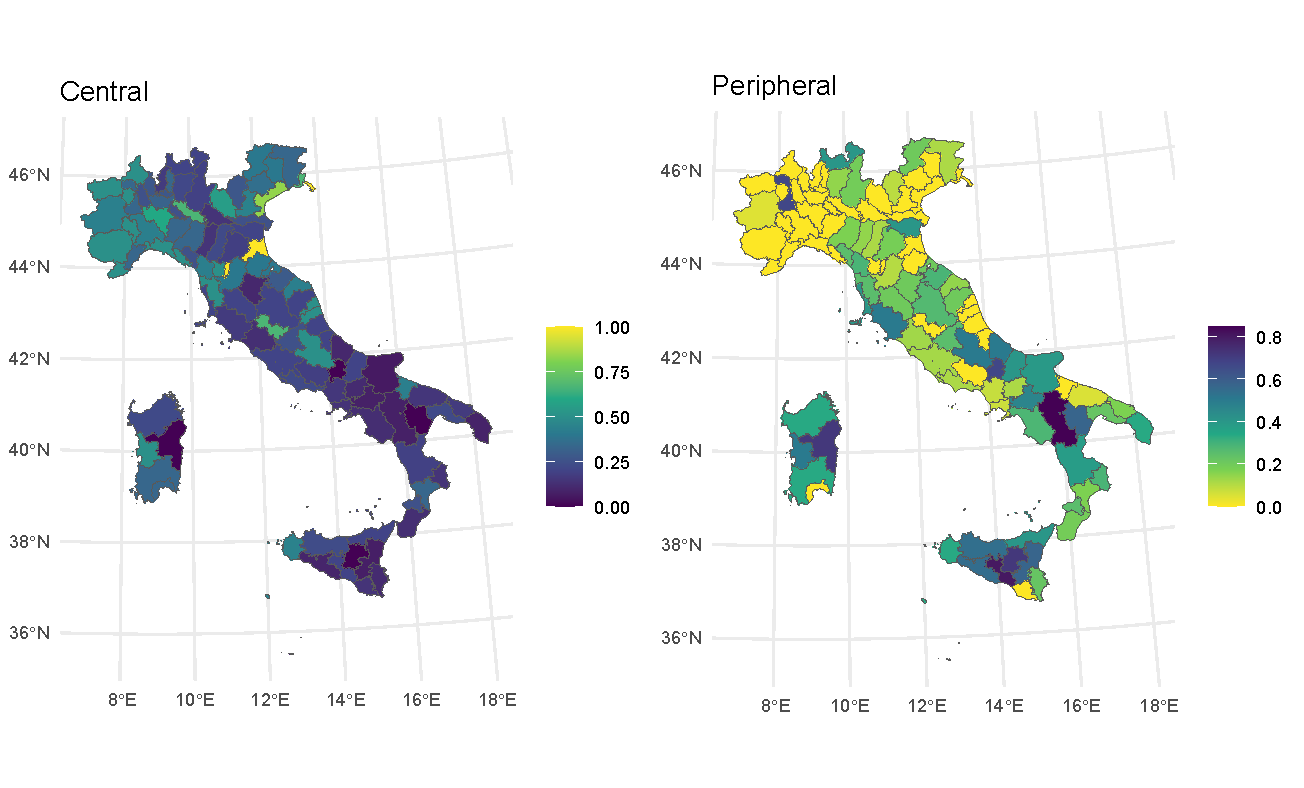
\includegraphics[width=0.9\textwidth]{Invalsi/X_prov_1.pdf} \\%[1ex] 
    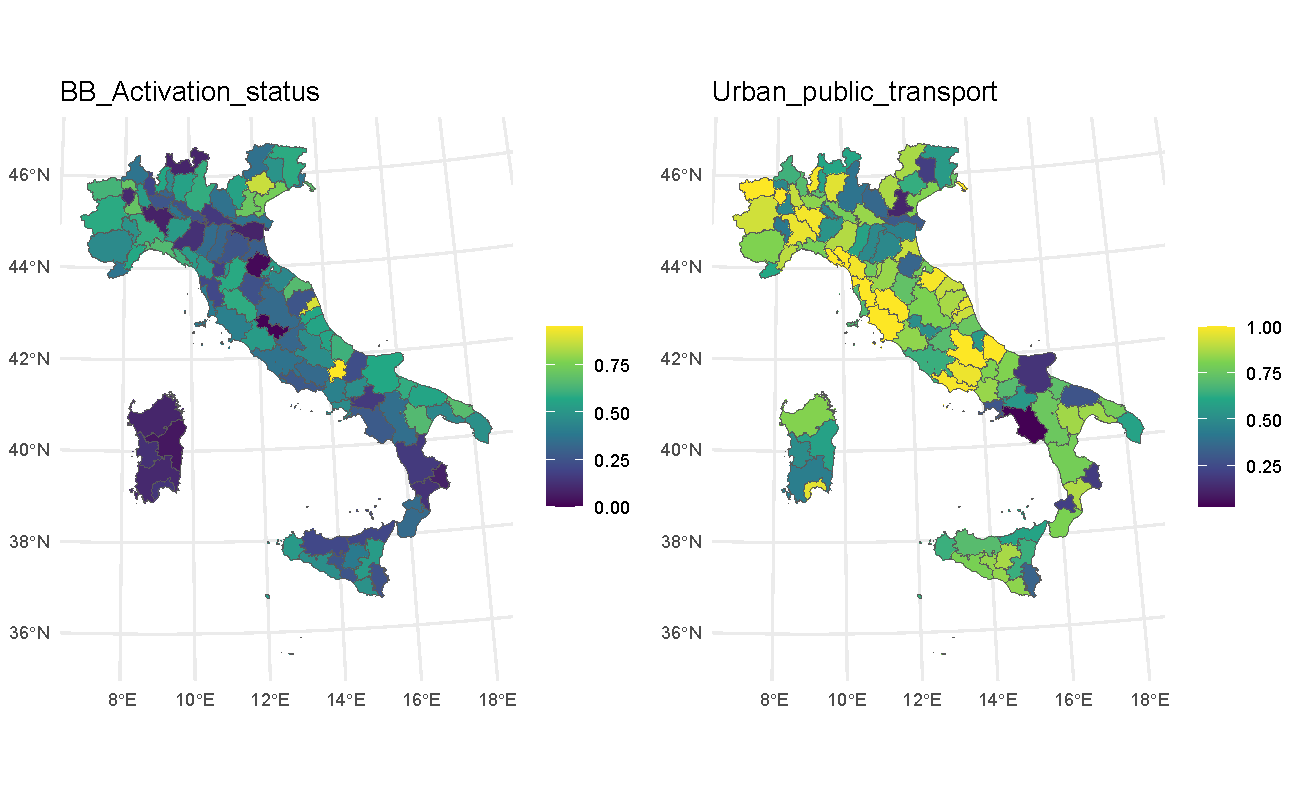
\includegraphics[width=0.9\textwidth]{Invalsi/X_prov_2.pdf} 
    \caption{Upper panel: proportion of central (left) and peripheral (right) municipalities per province.
    Lower panel: ultra-broadband availability (left) and urban transport accessibility (right) per province.}
    \label{fig:Xprov}
\end{figure}
%\begin{figure}
  %\centering
  %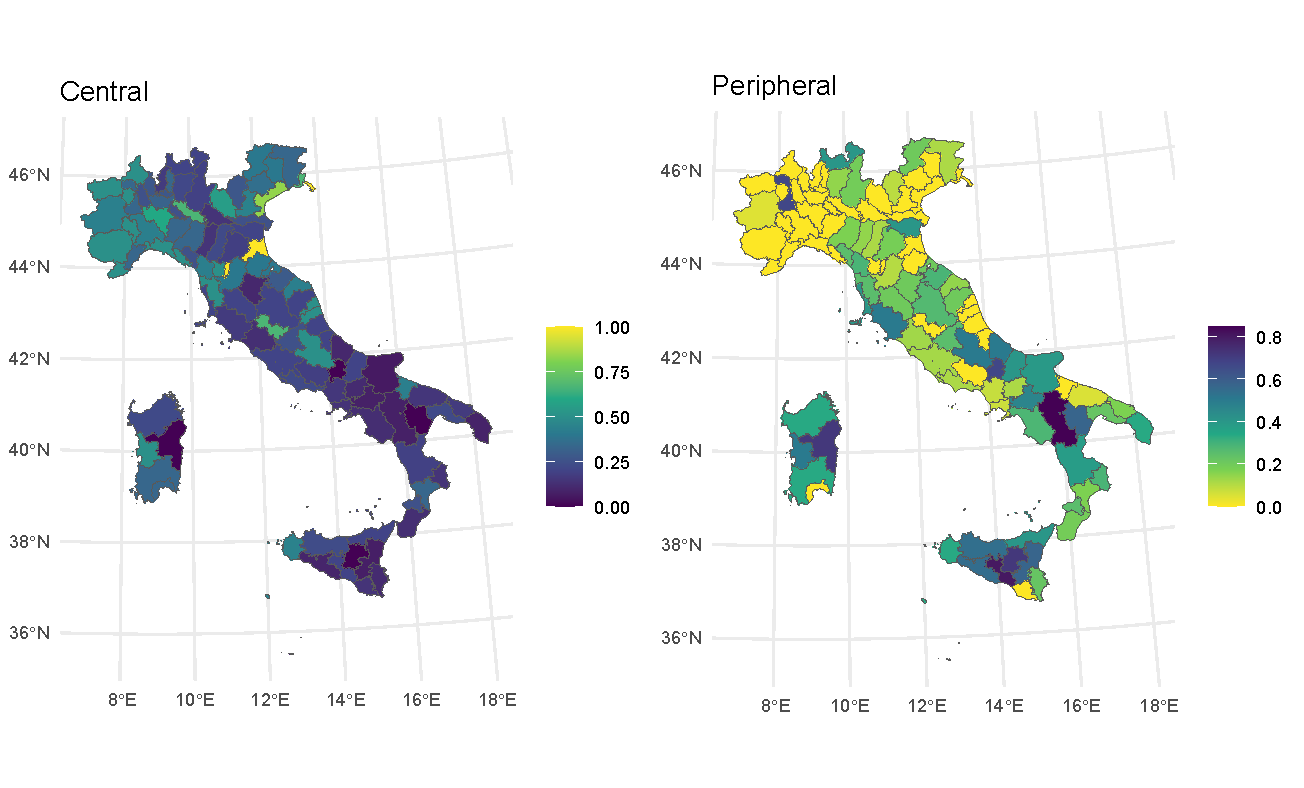
\includegraphics[width=0.9\textwidth]{Invalsi/X_prov_1.pdf} 
  %\caption{Proportion of central (left) and peripheral (right) municipalities per province}
  %\label{fig:Xprov1}
%\end{figure}
%\begin{figure}
 % \centering
  %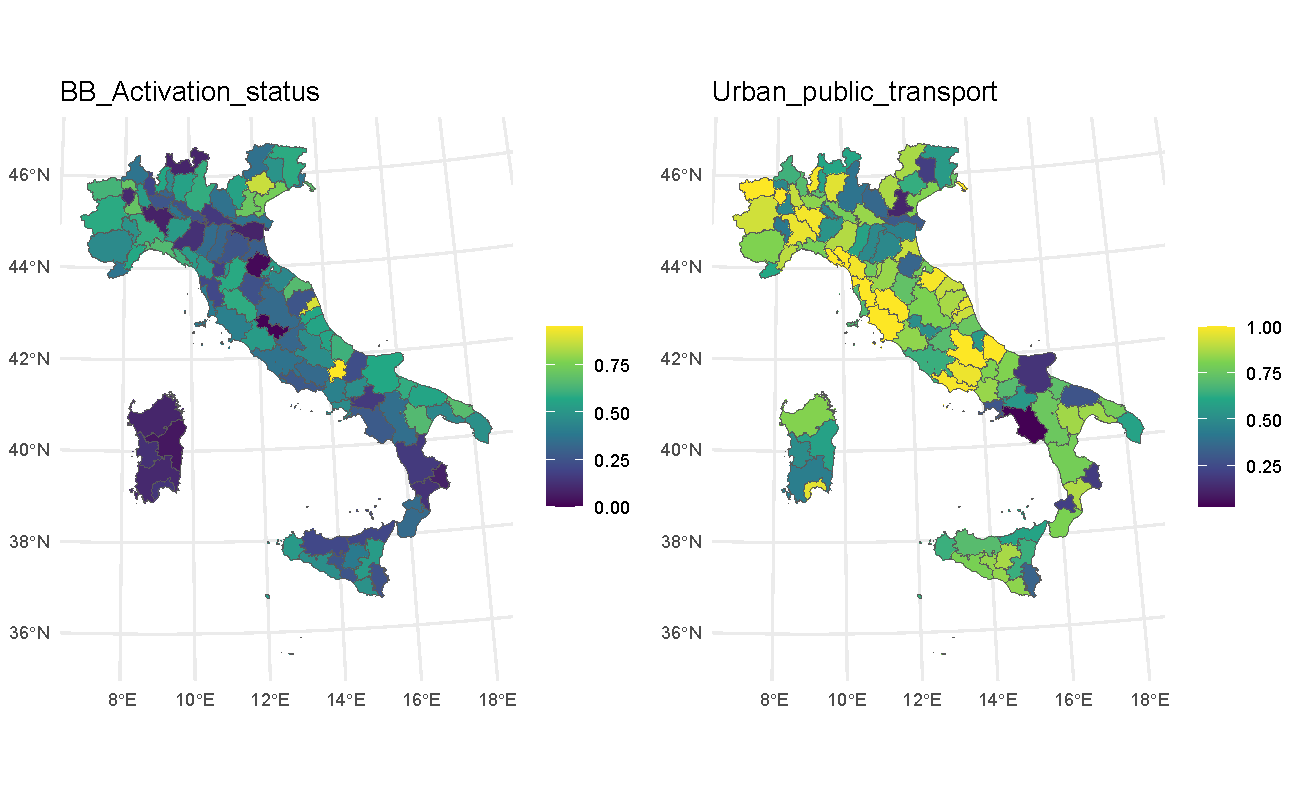
\includegraphics[width=0.9\textwidth]{Invalsi/X_prov_2.pdf} 
  %\caption{Ultra-BroadBand availability (left) and urban transport accessibility (right) per province}
  %\label{fig:Xprov2}
%\end{figure}
%


\begin{table}[ht]
\centering
\begin{tabular}{lrr}
Variable & $I$ & $I_\mathrm{std}$  \\ \hline
Central & 0.2705 & 4.1338   \\  
Peripheral & 0.4236 & 6.3447   \\
Broadband avail. & 0.1908 & 2.9234 \\ 
Urban transport & 0.0662 & 1.1072  \\  
\hline
\end{tabular}
\caption{Moran's $I$ and standardised $I$ values for province-level averages of auxiliary variables.}
\label{tab:MoranProv}
\end{table}

%When averaging covariates across infrastructural catchment areas, the values of $I_{std}$ are generally higher, and we find evidence for spatial autocorrelation also for the proportion of schools served by urban public transport.

%\begin{figure}
%  \centering
%  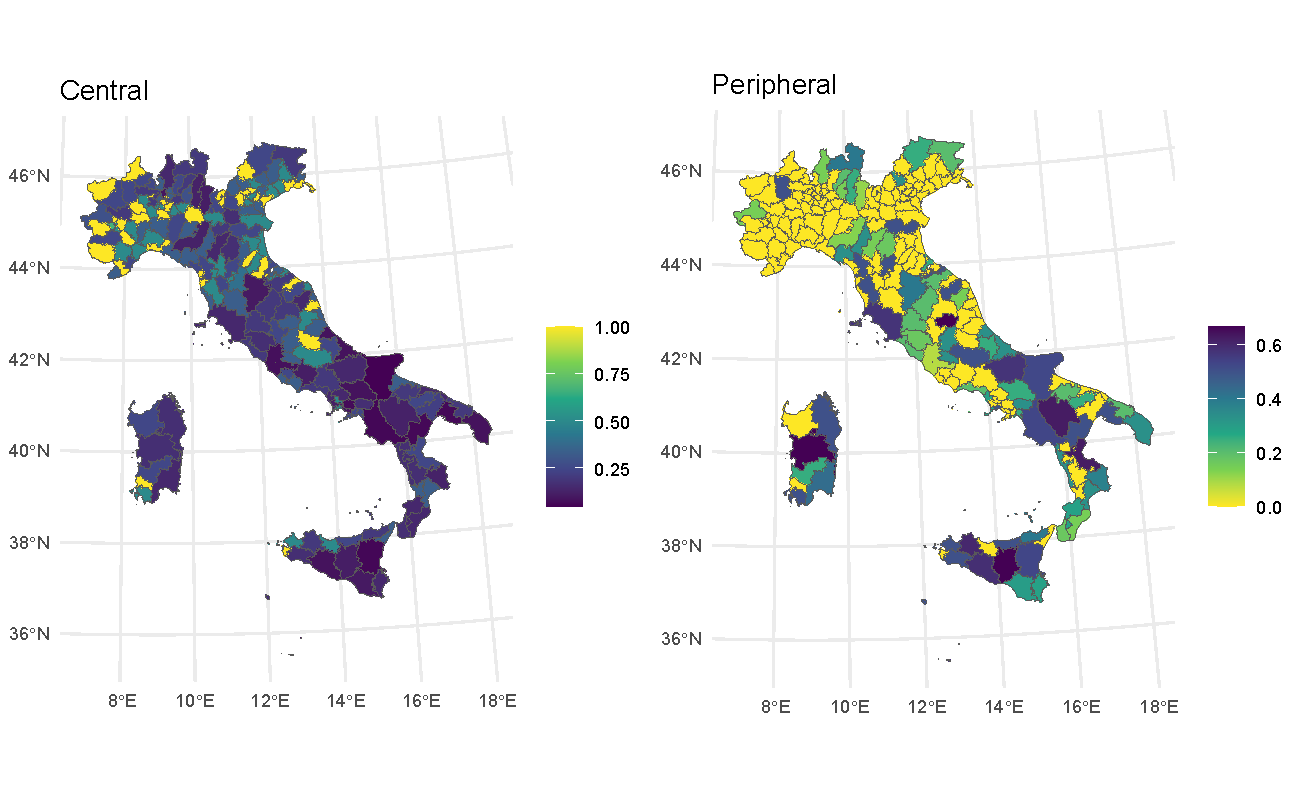
\includegraphics[width=0.9\textwidth]{Invalsi/X_pole_1.pdf} 
%  \caption{Proportion of central (left) and peripheral (right) municipalities per infrastructural catchment area}
%  \label{fig:Xpole1}
%\end{figure}
%\begin{figure}
%  \centering
%  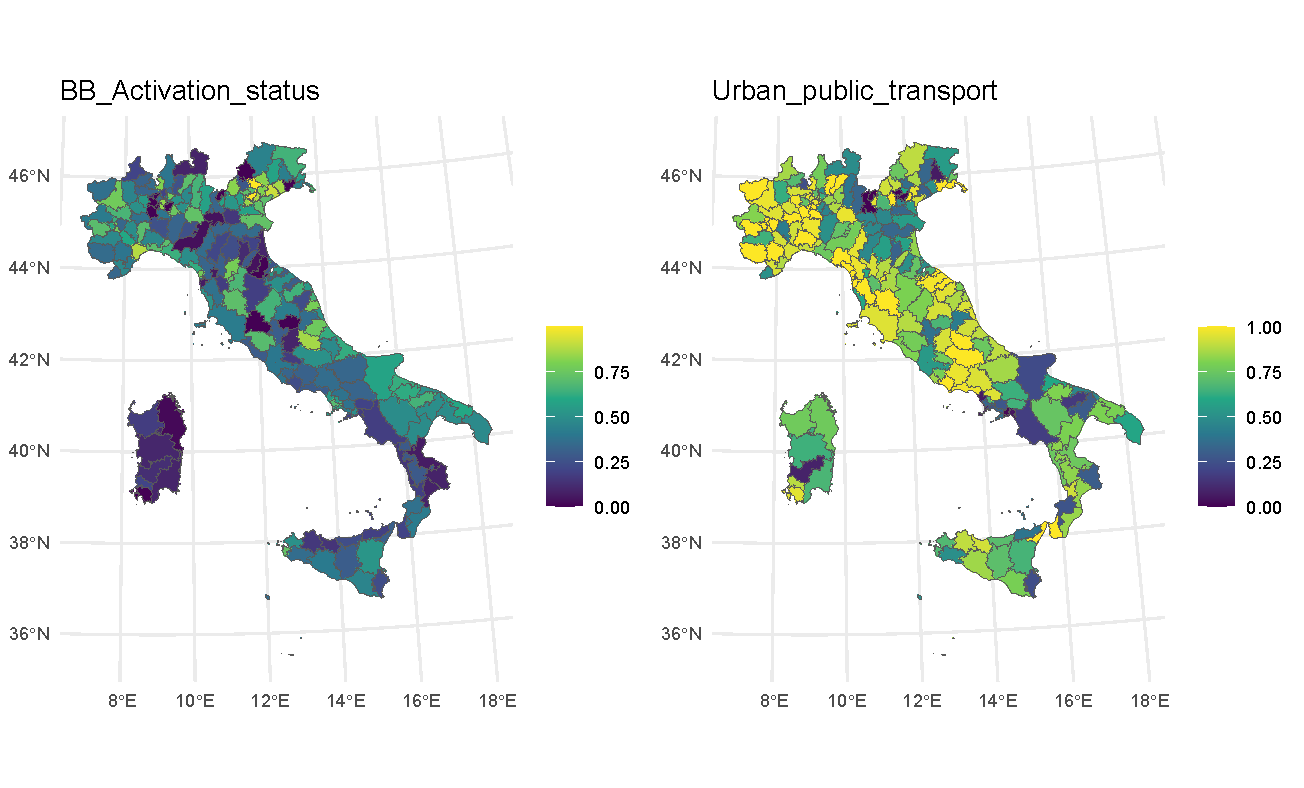
\includegraphics[width=0.9\textwidth]{Invalsi/X_pole_2.pdf} 
%  \caption{Ultra-BroadBand availability (left) and urban transport accessibility (right) per infrastructural catchment area}
%  \label{fig:Xpole2}
%\end{figure}


%\begin{table}[ht]
%\centering
%\begin{tabular}{lrr}
%Variable & $I$ & $I_{std}$             \\ \hline
%Central & 0.7100 & 15.4990             \\
%Peripheral & 0.2085  & 4.6337         \\ %1.79$\cdot 10^{-6}$
%Broadband avail. & 0.3089  & 6.8224  \\
%Urban transport &  0.3051 & 6.7238    \\
%\hline
%\end{tabular}
%\caption{Moran's $I$ values for infrastructural catchment area-level averages of auxiliary variables}
%\label{tab:MoranPole}
%\end{table}

%% --------- Autoregressive model ----------------------- %%
\section{A bivariate spatial model for student scores}\label{section:Model_outline}

In this Section, the general features of the bivariate spatial model for the Invalsi scores in Mathematics and Italian are outlined and general notation is introduced.
Assume the Invalsi scores in Mathematics and Italian $y = (y_1^{\top}, \, y_2^{\top})^{\top}$ are defined as a vector of length $2N$ and modelled as follows:\\
%$y := (y_1, \, y_2)$ are modelled as follows:\\
\begin{equation}
y =  \mathbf{\tilde{X}}  \, \beta \,  + 
\tilde{\mathbf{\xi}} \, \mathbf{\tilde{C}} \, \beta_C \,  +
\, \tilde{\mathbf{\xi}} \,z \, + \, \varepsilon
%%% N x 2 version - do not delete!!
%y = \, \mathbf{X} \, \beta \,  + 
%\xi \, \mathbf{C} \, \beta_C \,  
%+ \, \xi \, z \, + \, \varepsilon
\label{eq:model}
\end{equation}


where $\mathbf{\tilde{X}} := I_2 \otimes \mathbf{X}$, $\tilde{\xi} := I_2 \otimes \xi$ and $\mathbf{\tilde{C}} := I_2 \otimes \mathbf{C}$. $\mathbf{X}$ is the $N \times 4$ matrix of auxiliary variables (see Section \ref{Covariates}), and $\beta$ is a vector of fixed effects of length $8$. The $N \times n$ matrix $\xi$ is binary and maps the $n$ macro-areas onto $N$ municipalities. The $n \times 3$ matrix $\mathbf{C}$ is also binary and denotes which connected component (continent, Sicilia, Sardinia) each macro-area belongs to, $\beta_C$ is the vector of component-specific intercepts of length $6$. The bivariate latent spatial field $z = (z_1^{\top}, \, z_2^{\top})^{\top}$ is defined at the macro-area level and accounts for both the spatial variation and the correlation between Mathematics and Italian scores. Finally $\varepsilon = (\varepsilon_1^{\top} , \, \varepsilon_2^{\top})^{\top}$ is the matrix-valued random error, following the distribution:


\begin{equation}
\left\{
\begin{array}{ll}
\varepsilon_{1} \mid \omega_1 \overset{\text{iid}}{\sim}
N(\mathbf{0}, \omega_1)\\
\varepsilon_{2} \mid \omega_2, \alpha 
\overset{\text{iid}}{\sim} SN(m_{\omega_2, \alpha}, s_{\omega_2, \alpha}, \alpha)  
\end{array}
\right.
\label{eq:errors}
\end{equation} \\
$SN(\cdot)$ in \ref{eq:errors} denotes the Skew-Normal distribution \citep{SN} with location and scale parameters $m_{\alpha, \omega_2}$ and $ s_{\alpha, \omega_2}$ defined to ensure that $\mathbb{E}[\varepsilon_2 | \alpha] = 0 $ and $VAR[\varepsilon_2 | \alpha] = \omega_2$, and $\alpha$ is the shape parameter. This choice is due to the negative skewness in municipality-level Italian scores that neither auxiliary variables or spatial effects can explain (see Fig. \ref{fig:kernel} below). For interpretation reasons, in the remainder of this paper, we consider a transformation of $\alpha$, namely the skewness parameter $\gamma_1$, that has the property of lying approximately in the interval $]-1, 1[$:
$$
\gamma_{1} := \frac{4-\pi}{2}
\left(  \frac{2 \alpha^2}{\pi(1 + \alpha^2)} \right)^{\frac{3}{2}}
\left(  1 - \frac{2 \alpha^2}{\pi(1 + \alpha^2)} \right)^{-\frac{3}{2}}
$$
Following \cite{SNprior}, $\alpha$ is assigned a Penalised Complexity prior \cite{PC} with a given rate parameter $\lambda$. %\textcolor{orange}{, the reference model being the Gaussian likelihood}.
%$$
%\pi(\alpha) = \frac{1}{2}\lambda \displaystyle{e^{-\lambda D(\alpha)}}
%abs \left( \frac{d D(\alpha)}{d \alpha} \right)
%$$
%$D(\alpha)$ is the square root of an even polynomial in $\alpha$%, which approximates the Kullback-Leibler divergence from the Gaussian model
%Smaller values of $\lambda$ tend to move the probability mass away from zero, flattening the distribution of $\gamma_1$. 
$\lambda = 4$ is chosen based on empirical considerations, i.e. balancing model complexity and fit. However, the posterior distribution of the skewness parameter does not appear to be sensitive to the choice of $\lambda$ \citep{SNprior}.\\

Covariate effects $\beta$ have $N(0, 10^3)$ non-informative priors, while priors for intercepts in $\beta_C$ are set as $N(180, 10^3)$, according to the expected global mean of Invalsi ability scores (Section \ref{Par:Invalsi}).
Precision parameters for the error terms, namely $\omega_{1}$ and $\omega_2$, have independent Gamma vague priors with shape $10^{-3}$ and rate $10^{-3}$.

\subsection{Modelling the spatial component} \label{par:ICAR}
Considering the neighbourhood structure outlined in Section \ref{par:graph}, $z$ is modelled as a bivariate ICAR defined on the graph $\mathcal{G}$, following this conditional prior distribution at the spatial unit level for each $i$-th node, with $i \in [1, n]$:
\begin{equation}
z_{i} | z_{-i}, \Lambda \sim N \left(\sum_{j \sim i} \frac{w_{ij}}{d_i} z_{j}, \, \frac{1}{d_i} \Lambda^{-1}\right)
\label{eq:ICAR_local}
\end{equation}
where  $d_i := \sum_{s=1}^n w_{is}$ is the number of neighbours of node $i$ and $\Lambda$ is the precision parameter. This representation is a special case of the model developed by \citep[][theorem 2.1, corollary 2]{Mardia} and implies a joint Normal prior on $z$ with zero mean and precision $\Lambda \otimes \mathbf{R}$,

\begin{equation}
\pi\left(z\mid \Lambda \right) =
\left( \frac{1}{2 \pi} \right)^{n-3}\sqrt{\mid \Lambda \otimes\mathbf{R}  \mid_{+}} \, \, 
 e^{\displaystyle{-\tfrac{1}{2}
\mathrm{vec}(z)'(\Lambda \otimes \mathbf{R} ) \mathrm{vec}(z)}}
\label{eq:ICAR}
\end{equation}

where $\mathbf{R} := \mathbf{D} - \mathbf{W}$ is the Laplacian matrix of the graph $\mathcal{G}$ with $3$ connected components and $\mathbf{D} = \mathrm{diag}(d_1, d_2 \ldots d_n)$ is the degree matrix of $\mathcal{G}$.
Since $\mathbf{R}$ is singular with rank deficiency $3$ and $\pi(z|\Lambda)$ is therefore improper \citep{Hodges2003}, it is necessary to constrain $z$ to sum to zero within each connected graph component \citep{ICAR}. 
This is the reason for adopting component-specific intercepts $\beta_C$ in equation \ref{eq:model}.

To ease the interpretation of $\Lambda$ as the precision parameter of $z$, it is possible to cleanse it from the effect of the neighbourhood structure by defining a scaled version of $\mathbf{R}$ \cite{Sorbye} and reparametrising the precision of $z$ accordingly.
Since $\mathcal{G}$ is disconnected, each component-specific block of $\mathbf{R}$ is multiplied by the relevant typical variance, namely the geometric mean of the diagonal of the corresponding block of its pseudoinverse, following the methodology proposed by \cite{Freni}. It is therefore possible to define a precision parameter $\Lambda_\mathrm{scaled}$ which is not confounded with graph-induced effects. The scaled precision is assigned a Wishart prior \citep{Gelman} with $2k+1$ degrees of freedom and scale parameter equal to the identity matrix, i.e. $\Lambda_\mathrm{scaled} \sim \mathrm{Wishart}_{k}( I_k, 2k+1)$, with $k=2$ \citep{INLAMSM}.


$$
\mathbf{R}_\mathrm{scaled} := \mathcal{P} \left( \bar{\sigma}_{C_1}^2 \mathbf{R_{C_1}} \oplus \bar{\sigma}_{C_2}^2 \mathbf{R_{C_2}}  
\oplus \bar{\sigma}_{C_3}^2 \mathbf{R_{C_3}} \right) \mathcal{P'}
$$
where $\mathcal{P}$ is an appropriate permutation matrix, $\mathbf{R_{C_i}}$ is the Laplacian of the $i$-th connected component of the graph and $\bar{\sigma}_{C_i}^2$ is the relevant typical variance. 



In \texttt{R-INLA}, precision scaling is implemented automatically for intrinsic models, like the univariate ICAR, through the option \texttt{scale.model} within the \texttt{inla()} function call; otherwise the scaled structure matrix for each component can be computed as a standalone object with \texttt{inla.scale.model()}. In the multivariate case, \texttt{INLAMSM} provides readily-defined models for which the user is required to provide the neighbourhood matrix $\mathbf{W}$ instead of the Laplacian (as different models with the same neighbourhood matrix have different structure matrices). Hence, to scale a multivariate ICAR model we derive $\mathbf{W}$ from the scaled Laplacian.

\subsection{Spatial confounding}


In our multilevel framework, the value of the $m$-th covariate $\mathbf{X_{\cdot m}}$ observed in municipality $h$ belonging to macro-area $i$ can be decomposed as
$$
x_{ih;m} = \bar{x}_{i;m} + \Delta x_{ih;m}
$$
being $\bar{x}_{i;m}$ the unweighted average value of the covariate within the $i$-th macro-area; the term $\Delta x_{ih;m}$ represents municipality-level noise. In matrix form, this decomposition is: $\mathbf{X}= \xi \bar{\mathbf{X}} + \mathbf{\Delta X}$, where $\bar{\mathbf{X}} = (\xi ^{\top} \xi)^{-1} \xi^{\top} \mathbf{X}$.

Consider the eigendecomposition of the Laplacian matrix \citep{Urdangarin24}: 
$$
\mathbf{R} = \mathbf{VLV}^{\top}
$$
where the eigenvalues in $\mathbf{L}$ are in decreasing order and the eigenvectors in $\mathbf{V}$ have a decreasing number of oscillations. 

Within a generic component of the connected graph, the eigenvector associated with the lowest non-null eigenvalue follows a linear spatial trend (i.e. the Fiedler vector of the relevant subgraph), the one related to the second non-null eigenvalue follows a quadratic trend (one oscillation), and so on.
For an appropriately chosen $n \times 4$ matrix $\mathbf{b}$, $\mathbf{\bar{X}}$ can be expressed as a linear combination of $\mathbf{V}$:
$$
\mathbf{\bar{X}} = \mathbf{Vb}
$$
Intuitively, the spatial component of $\mathbf{\bar{X}}$ is determined by the last columns of $\mathbf{V}$ \citep{Urdangarin24}: without loss of generality, $\mathbf{\bar{X}}$ is decomposed into:
$$
\mathbf{\bar{X} }= \mathbf{\bar{X}^{(NS)}} + \mathbf{\bar{X}^{(S)}} +\mathbf{ \bar{X}^{(0)}}
$$
where $\mathbf{\bar{X}^{(NS)}}$ is the nonspatial component, given by the linear combination of the first $n-G-K$ eigenvectors (with $G=3$ connected graph components), $\mathbf{\bar{X}^{(s)}}$ is the combination of the eigenvectors associated with the last $K$ nonzero eigenvalues and represents the spatial component, and $\mathbf{\bar{X}^{(0)}}$ is the combination of the $G=3$ eigenvectors in the null space of the Laplacian matrix, constant within each connected component. 
To remove spatial confounding, it is sufficient to consider $\xi \left(\mathbf{\bar{X}^{(NS)}} \right) + \mathbf{ \Delta X}$ as the covariate matrix in the regression model. 

%\textcolor{blue}{Applying the Spatial+2.0 methodology to our data implies shifting the value of explanatory variables by an additive correction defined at the macro-area level, namely $\mathbf{\bar{X}^{(S)}} + \mathbf{\bar{X}^{(0)}}$. For instance, for a generic $h$-th covariate the corresponding deconfounded values are $x_{i;h} -x_{i;h}^{(S)}-x_{i;h}^{(0)}$. Subsequently, to allow model comparisons addressed in Section \ref{Par:results}, deconfounded covariates are scaled to have the same global variance as the input ones.}

%$if a generic $h$-th covariate is binary, taking values $x_{i,j;h} \in \lbrace{0, 1\rbrace}$, the corresponding deconfounded values would belong to the couple $\lbrace -x_{i;h}^{(S)}-x_{i;h}^{(0)}, \, 1 -x_{i;h}^{(S)}-x_{i;h}^{(0)}\rbrace$. Subsequently, deconfounded covariates are then scaled to have the same global variance as the input ones.

In Figure \ref{fig:eigen_prov} the eigenvectors corresponding to the last two non-zero eigenvalues of $\mathbf{R}$ at the macro-area level of provinces for the continent graph component are plotted. It is possible to see that the second-last eigenvector follows a quadratic trend with one oscillation, whereas the last eigenvector follows a linear North-South trend.  

\begin{figure}
  \centering
  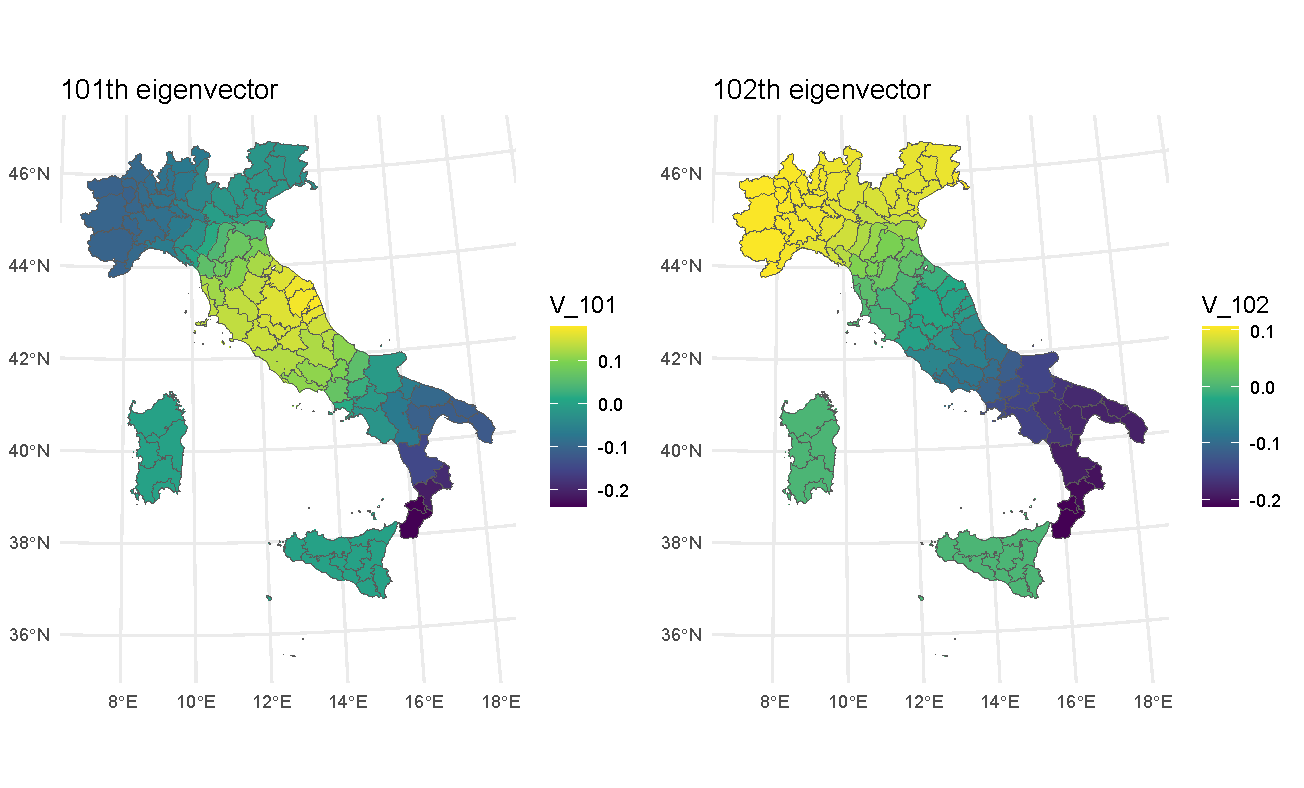
\includegraphics[width=0.9\textwidth]{Invalsi/eigen_prov.pdf} 
  \caption{Lowest frequency eigenvectors, provinces}
  \label{fig:eigen_prov}
\end{figure}

%\begin{figure}
%  \centering
%  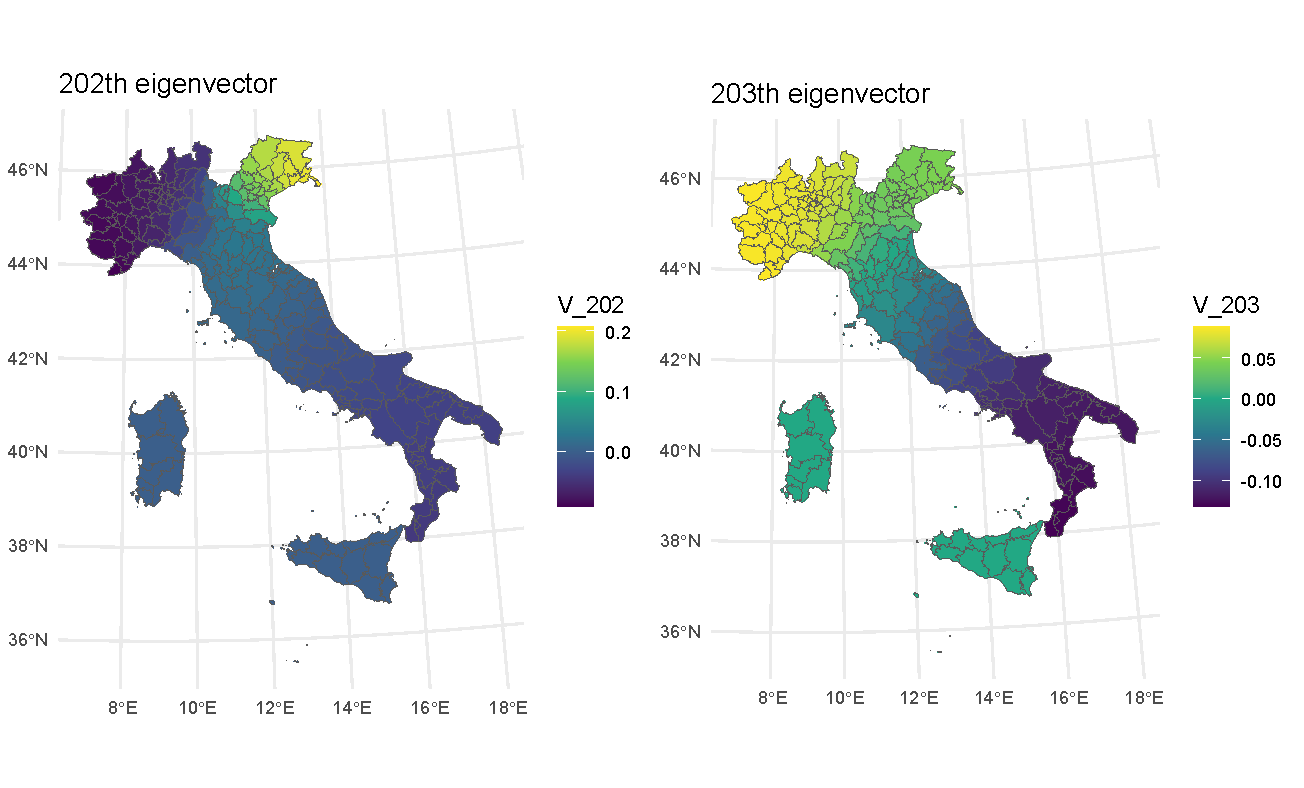
\includegraphics[width = 105mm]{Invalsi/eigen_pole.pdf} 
%  \caption{Lowest frequency eigenvectors, infrastructural catchment areas}
%  \label{fig:eigen_pole}
%\end{figure}

\subsubsection{Identification of the spatial variation in the covariates}\label{par:k}
The Spatial+ procedure requires the choice of the number $K$ of eigenvectors to define $\mathbf{\bar{X}^{(NS)}}$. A documented approach \citep{Urdangarin24, Lamouroux} is to choose the value of $K$ minimizing the Watanabe-Akaike Information Criterion \citep[WAIC,][]{WAIC}. Based on this method, our first strategy is searching for the optimal number of eigenvectors to be removed for each explanatory variable, subject to the following constraints.

When $z$ is defined at the province level (91 areas in the continent, 9 in Sicily, 5 in Sardinia), we remove a maximum of 9 eigenvectors in the continent, and 1 for each of the two islands, whereas when $z$ is defined at the level of infrastructural catchment areas (186 macro-areas in the continent, 13 in Sicily, 7 in Sardinia) we remove up to 18 eigenvectors from the continent, 2 from Sicily and 1 from Sardinia.

As an alternative strategy, we removed the smallest number of eigenvectors for $\mathbf{\bar{X}^{(NS)}}$ not to display evidence of autocorrelation according to Moran's $I$ index. %\textcolor{red}{, whose use is encouraged by its robustness to non-Normality \cite{Griffith} in datasets with at least $100$ observations.%} 
For the first three variables at the province level, removing the last $4$ eigenvectors leads to small standardized $I$ values ($0.79697$, $1.3854$, $1.2397$), suggesting that spatial structure in these variables is driven by a linear trend over the continent, as seen in Figure \ref{fig:Xprov}. For infrastructural catchment areas, doing the same thing with the proportion of central and peripheral municipalities would lead to standardized $I$ values of $1.2522$ and $0.4598$ respectively; again, this can be interpreted as the presence of a linear trend. For the last two covariates, instead, it is necessary to remove a higher amount of eigenvectors, which suggests the presence of spatial variation on a smaller scale before accepting the hypothesis of no spatial autocorrelation.

Details on the removal patterns are shown. The continent has 91 provinces and 186 infrastructural catchment areas; Sicily has 9 provinces and 13 infrastructural catchment areas; Sardinia has 5 provinces and 7 infrastructural catchment areas. The last eigenvector is constant within each component.
Patterns S+(1) and S+(3) are the simplest ones allowing to shrink the value of the standardised Moran's index below the $95$-th percentile of the Standard Normal distribution. At the province level, it is sufficient to remove the last 4 eigenvectors; at the level of infrastructural catchment areas this is only sufficient for the first two covariates, while more eigenvectors, corresponding to higher order trends, need to be removed for what concerns the other two variables. Pattern S+(2) allows, to the best of our findings, for the best ICAR fitting at the province level; S+(4) does the same at the level of infrastructural catchment areas; S+(5) and S+(6) serve the same purposes but for the PCAR model. In Figure \ref{fig:X_prov_nosp_1} the first two columns of $\mathbf{\bar{X}^{(NS)}}$ are shown, i.e. the province-level proportion of central and peripheral municipalities, using the S+(2) correction. Original values of these variables are in the upper panel of Figure \ref{fig:Xprov}.


\begin{table}[ht]
\resizebox{\textwidth}{!}{
\begin{tabular}{lll|rrrr}
\toprule
Pattern & level & Component & Central & Peripheral & BB Activation & Urban transport \\
\midrule
\multirow{3}{*}{S+(1)} & \multirow{3}{*}{Prov} & Continent & 2 & 2 & 2 & 0 \\
                       &                       & Sicily & 1 & 1 & 1 & 0 \\
                       &                       & Sardinia & 1 & 1 & 1 & 0 \\
\multirow{3}{*}{S+(2)} & \multirow{3}{*}{Prov} & Continent & 5 & 4 & 5 & 0 \\
                       &                       & Sicily & 1 & 1 & 1 & 0 \\
                       &                       & Sardinia & 1 & 1 & 1 & 0 \\
\multirow{3}{*}{S+(3)} & \multirow{3}{*}{Pole} & Continent & 2 & 2 & 10$^{*}$ & 13 \\
                       &                       & Sicily & 1 & 1 & 1 & 1 \\
                       &                       & Sardinia & 1 & 1 & 1 & 1 \\
\multirow{3}{*}{S+(4)} & \multirow{3}{*}{Pole} & Continent & 8 & 8 & 9 & 10 \\
                       &                       & Sicily & 2 & 1 & 1 & 1 \\
                       &                       & Sardinia & 1 & 1 & 1 & 1 \\
\multirow{3}{*}{S+(5)} & \multirow{3}{*}{Prov} & Continent & 5 & 4 & 6 & 0 \\
                       &                       & Sicily & 1 & 1 & 1 & 0 \\
                       &                       & Sardinia & 1 & 1 & 1 & 0 \\
\multirow{3}{*}{S+(6)} & \multirow{3}{*}{Pole} & Continent & 9 & 8 & 7 & 13 \\
                       &                       & Sicily & 2 & 1 & 1 & 2 \\
                       &                       & Sardinia & 1 & 1 & 1 & 1 \\

\bottomrule
\end{tabular}
}
\caption{Eigenvectors removal patterns for each explanatory variable.$^{*}$ In this case, eigenvectors removed are the 172th and 178-186th ones}
\label{tab:eigenremoval}
\end{table}


\begin{figure}[htbp]
    \centering
    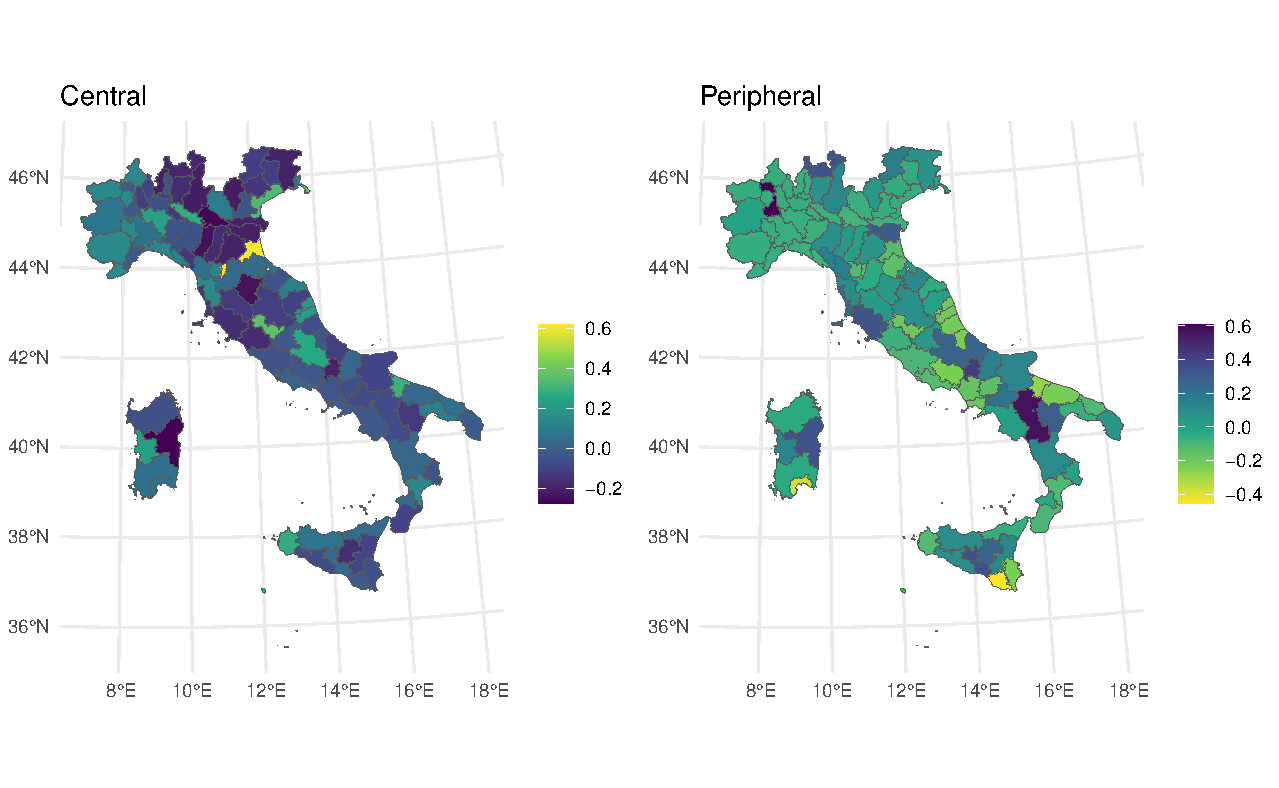
\includegraphics[width=0.9\textwidth]{Invalsi/X_prov_1_nosp_waic.pdf} \\%[1ex] 
    \caption{Proportion of central (left) and peripheral (right) municipalities per province once the spatial structure is removed by applying the S+(2) correction (see Table \ref{tab:eigenremoval}).}
    \label{fig:X_prov_nosp_1}
\end{figure}




% \begin{equation}
% \label{eq:marginals}
% \begin{aligned}
% \pi(\vartheta_i | y) = \int_{\Psi} \pi(\vartheta_i | y, \Psi) \pi(\Psi | y) d \Psi\\
% \pi(\Psi_l|y) = \int_{\Psi_{-l}} \pi(\Psi | y) d\Psi_{-l}
% \end{aligned}
% \end{equation}

 %%% Do not delete equation below %%%%%%%%%%%%%%%%%%%%%%%%%%%%%%%%
%\begin{equation}
%\pi_G(\vartheta | y, \Psi) \propto e^{\displaystyle {\frac{1}{2} (\vartheta - \mu_\Psi)' 
%\mathbf{H \mathrm{ln} f(\mu_\Psi, y | \Psi)} (\vartheta - \mu_\Psi)}}
%\label{eq:GaussianApprox}
%\end{equation}
%Where the $H$ operator denotes the Hessian matrix. Then, the joint posterior of hyperparameters $f(\Psi | y)$ can be computed, setting $\vartheta = \mu_\Psi$. 
%%% Do not delete equation above %%%%%%%%%%%%%%%%%%%%%%%%%%%%%%%%%


\subsection{Model assessment} \label{par:criteria}

In this Section, some alternative model formulations are compared using a set of selection criteria internally computed by \texttt{R-INLA}: the negative Log Pseudo Marginal Likelihood \citep[LPML,][]{Geisser, Gelfand}, i.e. minus the logarithmic sum of the Conditional Predictive Ordinates \citep{CPO, CPOINLA}, and the Watanabe-Akaike Information criterion \citep[WAIC,][]{WAIC}, following the formulation of \cite{GelmanWAIC}, the Deviance Information Criterion \citep[DIC,][]{DIC}, alongside with the Mean Squared Error of posterior predictive response averages.


The Conditional Predictive Ordinate is a leave-one-out cross-validatory diagnostic given for a generic $j$-th observation from the $h$-th variable, with $j \in [1, N]$ and $h \in [1,2]$, by: 
$$
\mathrm{CPO}_{j,h} := \pi(y_{j,h} \mid y_{-(j,h)})
$$  %% = \frac{\pi(y)}{\pi(y_{-j})}
Low CPO values denote "surprising" observations and, hence, possible outliers. Details on how the CPO is computed in \texttt{R-INLA} are provided by \cite{CPOINLA}. Here, we compare models through the logarithmic sum of CPOs changed of sign \cite{Geisser}. %, $\displaystyle{- \sum_{h=1}^2 \sum_{j = 1}^N \mathrm{ln}\, CPO_{j,h}}$ in our case. \\

The Deviance Information Criterion (DIC, \cite{DIC}) is given by:
$$
\mathrm{DIC} := P_D + \mathbb{E}[D(\vartheta, \Psi) \mid y]
$$
Where $$P_D = \mathbb{E}[D(\vartheta, \Psi)] - D(\hat{\vartheta}, \hat{\Psi})$$ denotes the effective number of parameters or unconstrained parameters and measures model complexity, $D(\vartheta, \Psi) = -2 \mathrm{ln} \pi(y \mid \vartheta, \Psi)$ being the model deviance, whose expectation measures the goodness of fit. Following \cite{INLA} we define $\hat{\vartheta}$ as $\mathbb{E}[\vartheta | y]$ and $\hat{\Psi}$  as the posterior mode of $\Psi$, this latter choice being due to the skewness in $\pi(\Psi | y)$. We show both the effective number of parameters and the expected deviance alongside the DIC.
 
The Watanabe-Akaike Information Criterion \cite{WAIC}, also known as Widely Applicable Information Criterion, is also useful in balancing model complexity and goodness of fit, the former being measured as $\mathrm{Var}[\mathrm{ln} \pi(y |\vartheta, \Psi)]$. An interesting feature of the WAIC is given by its averaging the likelihood over $\vartheta$ and $\Phi$ rather than using point estimates (\cite{GelmanWAIC}). We use the formulation provided by \cite{GelmanWAIC}. \\
 

$$
WAIC = 2 \sum_{j=1}^N VAR[\mathrm{ln} \pi(y_j |\vartheta, \Psi)]
- 2 \sum_{j=1}^N  \mathrm{ln} \mathbb{E}[\pi(y_j | \vartheta, \Psi)]
$$

%%Lastly we compute the Mean Square Error (MSE) of the expected value of linear predictors, a purely goodness-of-fit metric, only informative for point estimates.
%All selection criteria, except for the MSE, are internally computed by \texttt{R-INLA}.

Models defined with ICAR random effects are compared in Table \ref{tab:ICAR_diagnostics}. "Base" and "RSR" denote the model with no correction for spatial confounding and the RSR model respectively.
S+(1) and S+(2) are Spatial+2.0 models with province-level latent effects with two different eigenvector removal patterns: the former is the most conservative one for which no evidence for autocorrelation in the covariates is found (see Section \ref{par:X}), the latter is the one with smallest WAIC.
S+(3) and S+(4) are the Spatial+2.0 models developed with the same strategy but with latent effects defined at the level of infrastructural catchment areas. Detailed eigenvector removal patterns are shown in Appendix \ref{Appendix:A}.

Removing spatial autocorrelation from covariates based on Moran's test allows for some barely noticeable improvements in inference. Using finer support for the latent effects improves the fitting but this gain is outweighed by increased complexity (overall, the DIC increases).The model with province-level spatial effects is overall preferable based on all three metrics WAIC, DIC and LPML.
%
RSR appears to perform poorly in both cases if compared to the base model. Furthermore, posterior means of $\beta$ obtained by RSR result quite close to those of the nonspatial model, while credible intervals are narrower, which is consistent with the lesser coverage of Type-S errors in RSR models \citep{Khan}. 

In Appendix \ref{Appendix:B} the results of a broader set of models are shown, including models with no random effects, with unstructured random effects and with two independent ICAR random effects; a focus on the estimates of $\beta$ under the nonspatial model and under RSR is in Appendix \ref{Appendix:null_RSR}. 

Lastly, in Appendix \ref{Appendix:C} the results of a different model, the proper CAR \citep{PCAR_Gelfand}, are summarised. The core feature of this formulation is introducing an additional parameter to account for the strength of spatial association.


\begin{table}[ht]
\resizebox{\textwidth}{!}{
\centering
\begin{tabular}{llrrrrrr}
  \toprule
  $z$ level & Model & -LPML & WAIC & DIC & MSE \\ 
  \midrule
  Prov & Base &6689.917 & 13379.149 & 13379.808 & 235.551 \\ %& 13307.056 & 72.752
  Prov & RSR  &6764.094 & 13526.761 & 13526.476 & 251.886 \\ %& 13440.811 & 85.665 
  Prov & S+(1)&6689.672 & 13378.651 & 13379.311 & 235.326 \\ %& 13306.071 & 73.239 
  Prov & S+(2)&\textbf{6689.500} & \textbf{13378.303} & \textbf{13378.909} & 235.189 \\  \midrule %& 13305.406 & 73.502
  Pole & Base &6694.435 & 13387.776 & 13388.726 & 232.320 \\ %13300.529 & 88.197 
  Pole & RSR  &6754.037 & 13505.502 & 13507.315 & 239.313 \\ %& 13388.609 & 118.706
  Pole & S+(3)&6694.443 & 13387.747 & 13388.711 & \textbf{231.811} \\ %& 13298.501 & 90.210
  Pole & S+(4)&6694.055 & 13387.018 & 13387.948 & 231.838 \\ %& 13298.904 & 89.044
   \bottomrule 
   
\end{tabular}
}
\caption{Model diagnostics for 8 ICAR model formulations: spatial aggregation level of $z$, spatial confounding treatment, negative Log Pseudo Marginal Likelihood, Watanabe-Akaike Information criterion, Deviance Information Criterion, Mean Squared Error of posterior predictive response averages.}
\label{tab:ICAR_diagnostics}
\end{table}
%% --------- Findings ----------------------------------- %%
\section{Results}\label{Par:results} \label{section:results}

In Table \ref{tab:fix} the estimated effects of covariates for the province-level ICAR are resumed, under both the base formulation and the S+(2) modification. Boundaries of credible intervals correspond to the $5$-th and $95$-th percentiles. Covariates in the deconfounded model have been scaled to keep the same variance as in the base model.

\begin{table}[ht]
\resizebox{\textwidth}{!}{
\centering
\begin{tabular}{ll|rrrr|rrrr}
  \toprule
  && \multicolumn{4}{c|}{Base model} & \multicolumn{4}{c}{S+(2)}\\
 & Subj & mean & sd & LB & UB & mean & sd & LB & UB \\ 
  \midrule
Continent & MAT & 191.399 & 0.961 & 189.515 & 193.285 & 193.332 & 0.855 & 191.656 & 195.009 \\ 
  Continent & ITA & 187.107 & 0.999 & 185.137 & 189.056 & 188.585 & 0.863 & 186.886 & 190.270 \\ 
  Sicily & MAT & 177.764 & 1.496 & 174.829 & 180.698 & 178.386 & 1.369 & 175.702 & 181.070 \\ 
  Sicily & ITA & 176.884 & 1.550 & 173.835 & 179.915 & 177.273 & 1.417 & 174.489 & 180.046 \\ 
  Sardinia & MAT & 174.325 & 2.197 & 170.017 & 178.634 & 174.561 & 2.159 & 170.327 & 178.795 \\ 
  Sardinia & ITA & 171.914 & 2.267 & 167.460 & 176.351 & 172.126 & 2.208 & 167.790 & 176.450 \\ 
  Central & MAT & 2.706 & 0.910 & 0.922 & 4.490 & 2.527 & 0.890 & 0.781 & 4.273 \\ 
  Central & ITA & 2.379 & 0.996 & 0.433 & 4.338 & 2.460 & 0.979 & 0.547 & 4.386 \\ 
  Peripheral & MAT & -2.200 & 1.005 & -4.171 & -0.228 & -2.018 & 0.958 & -3.897 & -0.139 \\ 
  Peripheral & ITA & -1.845 & 1.049 & -3.901 & 0.215 & -1.793 & 1.000 & -3.753 & 0.170 \\ 
  BB Activation & MAT & 3.331 & 1.074 & 1.226 & 5.437 & 3.262 & 1.049 & 1.205 & 5.319 \\ 
  BB Activation & ITA & 2.296 & 1.126 & 0.090 & 4.509 & 2.130 & 1.100 & -0.024 & 4.291 \\ 
  Urban transport & MAT & 2.466 & 1.043 & 0.420 & 4.513 & 2.501 & 1.044 & 0.453 & 4.549 \\ 
  Urban transport & ITA & 2.841 & 1.060 & 0.765 & 4.924 & 2.838 & 1.060 & 0.762 & 4.919 \\ 
   \bottomrule
\end{tabular}
}
\caption{Posterior summaries of intercepts and covariate effects when $z$ is defined as a province-level ICAR, under the base model and the Spatial+2.0 model (optimal combination of eigenvector removal under the WAIC metric)}
\label{tab:fix}
\end{table}

Modelling Italian scores appears to be generally subject to higher uncertainty. For both subjects, differences between the continent and the islands are strong: almost $15$ Invalsi points on average between the continent and Sicily, more than $15$ points between the continent and Sardinia, with non-overlapping credible intervals. Central municipalities have an expected advantage of $2.706$ points over intermediate municipalities in Mathematics test, while this expectation slightly falls to $2.527$ points once the share of infrastructural poles in each province is corrected with S+(2). The relative effect of central municipalities on Italian scores is comparable and slightly lower. The difference between intermediate and peripheral municipalities is lower in expected value and not even significant for Italian scores. A municipality in which all schools are provided with ultra-broadband connection has an expected advantage of more than $3$ Invalsi points in the Mathematics score over one in which the connection is completely lacking, the effect being weaker on Italian scores (and possibly not significant once the spatial structure is removed from the covariate). Lastly, the availability of urban public transport is associated with a significant advantage in Invalsi scores, since a municipality where all schools are reachable has an expected advantage of almost $2.5$ points in Mathematics scores and about $2.8$ points in Italian scores. 

In Figure \ref {fig:zprov} the expected spatial effect $\mathbb{E}[z|y]$ under the S+(2) model is plotted. %Also taking into account the four auxiliary variables, 
Territorial gaps in Invalsi scores are severe, as one can argue from the range of $\mathbb{E}[z|y]$. Focusing on the continent, the Calabria region appears particularly vulnerable, while Lombardia turns out to be the most advantaged region. 

In Figure \ref{fig:yhatmun} the predicted values of $y$ are shown, using the same model. The model captures the spatial trend, but still leaves a high municipality-level noise unexplained, as the high error variances suggest ($\omega_1$ and $\omega_2$ in Table \ref{tab:hyperpar}). 

The highest scores are estimated in the municipalities of Lecco (Lombardia), with expected scores of $216.072$ points in Mathematics (observed score of $214.042$ points) and $207.637$ points in Italian (observed $204.990$ points) and Merate (province of Lecco), with expected scores of $216.133$ points in Mathematics (observed score $229.352$ points) and $207.274$ points in Italian (observed value $216.045$ points). 

Lowest scores in Mathematics are estimated in the municipalities of La Maddalena (province of Sassari, Sardinia) at $169.351$ points and Oppido Mamertina (province of Reggio Calabria) at $170.301$ points  (observed $165.814$ and $170.105$ points respectively). Lowest scores in Italian are estimated in the municipalities of La Maddalena at $170.016$ points  and Bosa (province of Oristano, Sardinia) at $169.787$ points (observed $168.071$ and $168.890$ points respectively).

%The highest scores are estimated in the municipalities of Lecco (Lombardia), with expected scores of $216.072$ points in Mathematics (standard deviation of the linear predictor $2.616$ points, observed score of $214.042$ points) and $207.637$ points in Italian (predictor s.d. $2.343$ points, observed score $204.990$ points) and Merate (province of Lecco), with expected scores of $216.133$ points in Mathematics (predictor s.d. $2.657$ points, observed score $229.352$ points) and $207.274$ points in Italian (predictor s.d. $2.388$ points, observed value $216.045$ points). Lowest scores in Mathematics are estimated in the municipalities of La Maddalena (province of Sassari, Sardinia region) at $169.351$ points(predictor s.d. $2.960$ points, observed score $165.814$ points) and Oppido Mamertina (province of Reggio Calabria, Calabria region) at $170.301$ points (predictor s.d. $2.351$ points, observed score $170.105$ points). Lowest scores in Italian are estimated in the municipalities of La Maddalena at $170.016$ points (predictor s.d. $2.806$ points, observed score $168.071$ points) and Bosa (province of Oristano, Sardinia) at $169.787$ points (predictor s.d. $3.770$ points, observed score $168.890$ points).

%of Lecco and Como (Lombardy) with $17.470$ and $15.568$ points in Mathematics (standard deviations $2.484$ and $2.423$) and $13.840$ and $12.318$ points in Italian (standard deviation $2.143$ and $2.081$) respectively. The record disadvantage is estimated in the provinces of Cosenza and Crotone (Calabria) with $-20.381$ and $-18.839$ points in Mathematics (standard deviations $2.093$ and $2.674$) and $-15.908$ and $-14.450$ points in Italian (standard deviations $1.962$ and $2.283$) respectively.

\begin{figure}
  \centering
  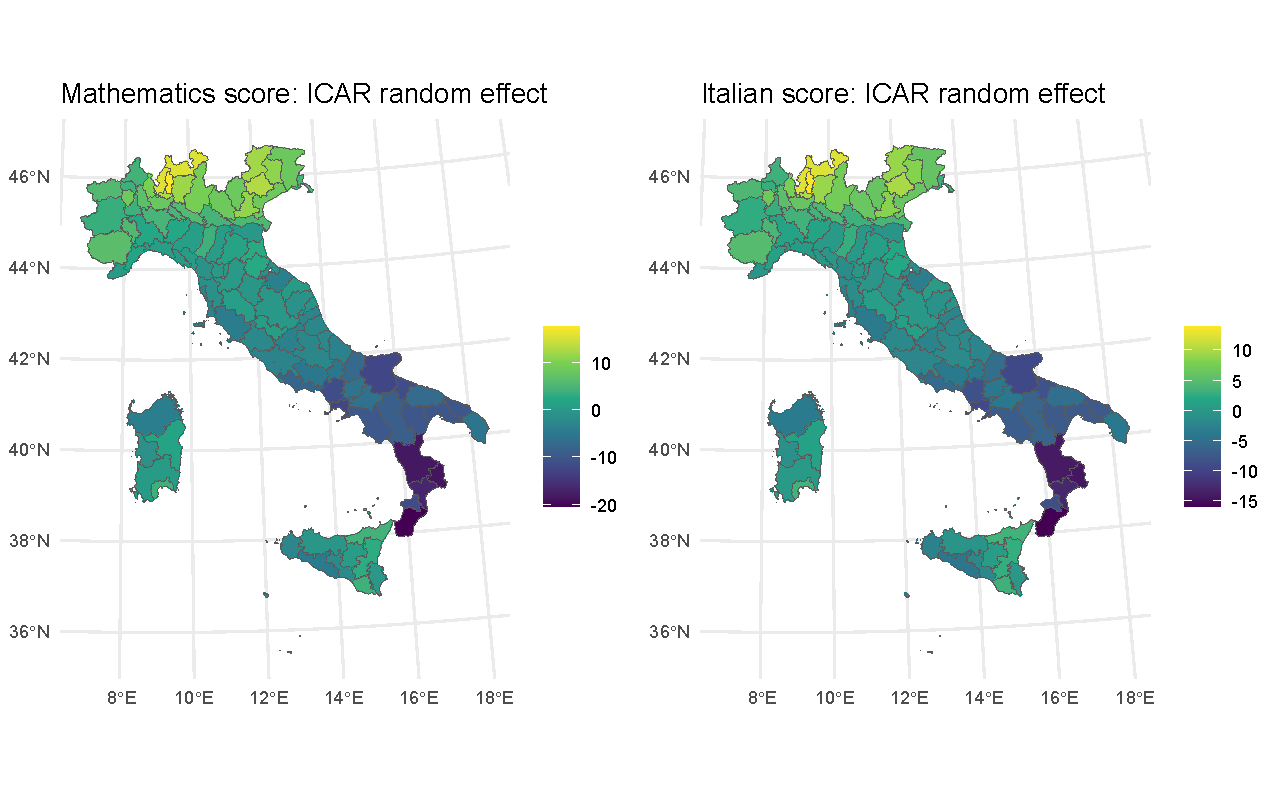
\includegraphics[width=0.9\textwidth]{Invalsi/z_IMCAR_spatplus_waic.pdf} 
  \caption{Expected values of $z$ modelled as a province-level ICAR and applying S+(2) correction}
  \label{fig:zprov}
\end{figure}

\begin{figure}
  \centering
  \includegraphics[width=0.9\textwidth]{Invalsi/yhat_mun_spatplus_waic.pdf} 
  \caption{Predicted values of Invalsi scores using as a province-level ICAR latent effect and applying the S+(2) correction}
  \label{fig:yhatmun}
\end{figure}

Finally, in Table \ref{tab:hyperpar} the posterior summaries for hyperparameters $\Psi$ are displayed. Please notice that the precision of $z$ has been scaled, hence variances $\sigma_1^2$ and $\sigma_2^2$ do not depend on the graph-induced effect. The variance of spatial effects is higher in Mathematics scores ($\sigma_1^2$), while Italian scores have a higher amount of unexplained noise ($\omega_2$). Correlation between the two scores is taken into account through the correlation between the two ICAR fields $\rho$, which turns out to be high, consistent with Figure \ref{fig:zprov}.
Lastly, the choice of modelling Italian scores as a Skew-Normal variable is corroborated by the posterior distribution of $\gamma_1$, whose credible interval ranges far from zero. Kernel density estimation of residuals in Italian scores % \textcolor{gray}{i.e. the difference between observed and predicted scores (SERVE SPECIFICARE?)} 
is shown in Figure \ref{fig:kernel}. Negative skewness is easily noticeable. Density is estimated by the Gaussian kernel, using the Silverman's thumb rule to define the bandwidth \citep[][Section 3.4.2]{Silverman}
\begin{figure}
  \centering
  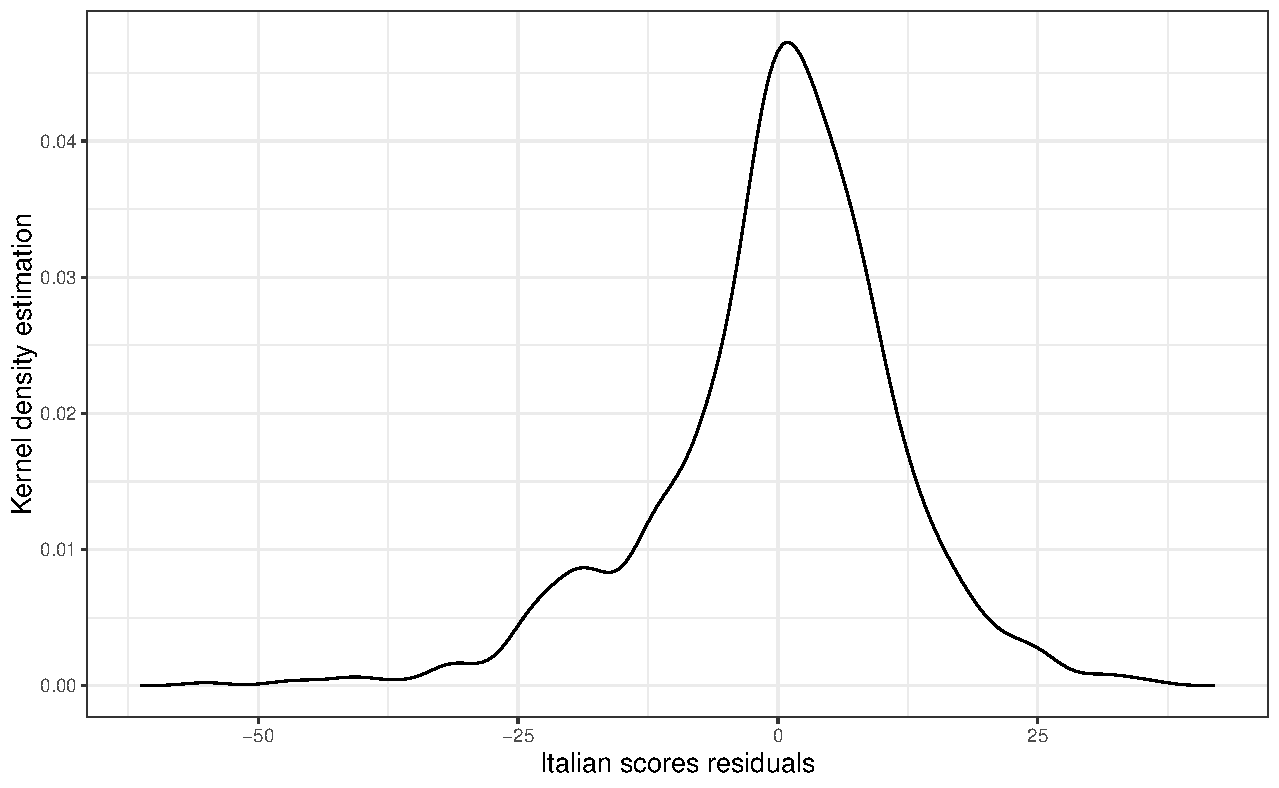
\includegraphics[width=0.6\textwidth]{Invalsi/KDE_ITA_base.pdf} 
  \caption{Kernel density estimation of the residuals of Italian scores under the S+(2) model}
  \label{fig:kernel}
\end{figure}


\begin{table}[ht]
\resizebox{\textwidth}{!}{
\centering
\begin{tabular}{ll|rrrr|rrrr}
  \toprule
  && \multicolumn{4}{c|}{Base model} & \multicolumn{4}{c}{S+(2)}\\
 & Subj & LB & Median & UB & sd & LB & Median & UB & sd \\ 
  \midrule
 $\sigma_1^2$ & MAT & 16.621 & 27.414 & 46.208 & 7.578 & 17.288 & 28.722 & 46.823 & 7.562 \\ 
 $\sigma_2^2$ & ITA  & 10.277 & 18.156 & 33.042 & 5.843 & 10.672 & 18.832 & 32.760 & 5.663 \\ 
 $\rho$ &     & 0.894 & 0.975 & 0.995 & 0.027 & 0.884 & 0.976 & 0.994 & 0.030 \\ 
  $\omega_1$ & MAT & 100.830 & 110.924 & 122.138 & 5.426 & 100.712 & 110.790 & 121.982 & 5.417 \\ 
  $\omega_2$ & ITA & 119.507 & 132.104 & 145.888 & 6.718 & 119.368 & 131.795 & 145.646 & 6.692 \\
  $\gamma_1$ & ITA & -0.493 & -0.371 & -0.232 & 0.067 & -0.493 & -0.369 & -0.232 & 0.066 \\ 
   \bottomrule
\end{tabular}
}
\caption{Posterior summaries of hyperparameters when $z$ is defined as a province-level ICAR, under the base model and the Spatial+2.0 model (optimal combination of eigenvector removal under the WAIC metric)}
\label{tab:hyperpar}
\end{table}

%% --------- Conclusion --------------------------------- %%
\section{Concluding remarks}

While a good body of literature studies student ability scores at the individual level, we have turned the analysis to a different framework, attempting to explain the geographical distribution of Invalsi scores based on infrastructural variables and using a multivariate spatial regression model. For a better understanding of the spatial variation, the precision of the spatial effect was scaled to account for discontinuities implied by the presence of two islands. The typical skew distribution in the Italian Invalsi scores was accounted for by relaxing the Normality assumption and fitting a Skew-Normal likelihood, with evidence for negative skewness. Lastly, to avoid explanatory variables being confounded with the spatial effect, we cleansed them from low-frequency spatial trends in estimating their effect on Invalsi scores.

The infrastructural state of schools and municipalities results in a significant impact on student performances, also when their effect is separated from spatial information. The classification of Italian municipalities into central, intermediate, and peripheral allows to report a noticeable advantage of the first to the second, while the difference between intermediate and peripheral municipalities is weaker. Our results do highlight the overall vulnerability of inner areas under the educational dimension.

Our analysis of Invalsi scores includes a spatially structured latent field defined at the level of macro-areas, either provinces or infrastructural catchment areas. We find that the between-macro-areas spatial effect is indeed a strong driver of Invalsi scores, in addition to between-municipalities factors. This confirms the strength of the territorial divides shaping many aspects of Italian society, especially the North-South gap.

Still keeping our focus on infrastructural explanatory variables, this analysis can undergo some possible developments: first and foremost it can be extended to different school grades and different years. The choice of statistical models, both in terms of likelihood and prior assumptions, could be extended as well, including more tailored models. The PCAR model, for instance, may represent a worthwhile extension, though questions like improving the interpretation of precision parameters remain open, further research being needful to this aim.

Overall, the mapping of infrastructure access and social vulnerability requires adequate statistical computational methods, and \texttt{R-INLA} appears a very flexible tool to this aim.















\begin{appendices}

\section{Extensive model comparison} \label{Appendix:B}
In Table \ref{tab:ICAR} all the models run throughout this analysis are compared. Two alternative strategies to approximate the full posterior of $\vartheta$ have been tested, namely the Variational Bayes and the Simplified Laplace approximations (respectively VB and SL, hereinafter). The former is implemented in the latest \texttt{R-INLA} framework and has been used to estimate the models whose results are summarised in Sections \ref{par:criteria} and \ref{section:results}. The latter allows to preserve information about skewness in the full conditional and is implemented in an older software framework. Due to the difficulties in locating the mode of $\Psi$, $y$ required to be centered at zero in the models approximated with the SL method.

Some additional model formulations are also compared: "NULL" denotes the model with no spatial effect (component-specific intercepts are still used); "IID" denotes the model with IID macroarea-level effects; "Ind. ICAR" denotes the model with two independent ICAR priors. The random intercept and the ICAR effect in the IID and independent ICAR models have an improper Uniform prior on the standard deviation. Models  S+(1), S+(2), S+(3), and S+(4)  are defined as in Appendix \ref{Appendix:A}. Alongside the selection criteria mentioned in Section \ref{par:criteria}, the two components of the DIC are shown, namely the expected deviance (Exp. Dev) and the effective number of parameters ($P_D$). The computational time of each model is shown as well, expressed in seconds. \\

This comparison highlights that the ICAR is more adequate to study Invalsi scores than both the null and IID models. In this latter case, point estimates are accurate (low MSE), but the high complexity suggests this may be due to overfitting. The correlated ICAR outperforms the independent one. The VB approximation also appears to be generally preferable over the SL.

 
\begin{table}[ht]
\centering
\resizebox{\textwidth}{!}{
\begin{tabular}{rlllrrrrrrrr}
  \hline
  $z$ level & Approx & Model & -LPML & WAIC & DIC & Exp. Dev. & $P_D$ & MSE & time \\ 
  \toprule

  Null & VB & Null & 6979.502 & 13959.022 & 13959.264 & 13942.292 & \textbf{16.972} & 346.158 & 2.038 \\ 
  Prov & VB & IID & 6765.015 & 13524.273 & 13523.594 & 13368.734 & 154.860 & 233.906 & 6.204 \\ 
  Prov & VB & Ind. ICAR & 6722.306 & 13443.342 & 13443.291 & 13355.484 & 87.807 & 239.622 & 7.389 \\ 
  Prov & VB & Base ICAR & 6689.917 & 13379.149 & 13379.808 & 13307.056 & 72.752 & 235.551 & 11.501 \\ 
  Prov & VB & ICAR RSR & 6764.094 & 13526.761 & 13526.476 & 13440.811 & 85.665 & 251.886 & 10.197 \\ 
  Prov & VB & ICAR S+(1) & 6689.672 & 13378.651 & 13379.311 & 13306.071 & 73.239 & 235.326 & 11.111 \\ 
  Prov & VB & ICAR S+(2) & \textbf{6689.500} & \textbf{13378.303} & \textbf{13378.909} & 13305.406 & 73.502 & 235.189 & 11.613 \\ 
  Pole & VB & IID & 6840.664 & 13669.514 & 13666.691 & 13452.671 & 214.020 & 236.693 & 5.613 \\ 
  Pole & VB & Ind. ICAR & 6755.812 & 13508.925 & 13508.602 & 13390.671 & 117.931 & 240.193 & 17.936 \\ 
  Pole & VB & Base ICAR & 6694.435 & 13387.776 & 13388.726 & 13300.529 & 88.197 & 232.320 & 12.178 \\ 
  Pole & VB & ICAR RSR & 6754.037 & 13505.502 & 13507.315 & 13388.609 & 118.706 & 239.313 & 14.593 \\ 
  Pole & VB & ICAR S+(3) & 6694.443 & 13387.747 & 13388.711 & \textbf{13298.501} & 90.210 & 231.811 & 13.932 \\ 
  Pole & VB & ICAR S+(4) & 6694.055 & 13387.018 & 13387.948 & 13298.904 & 89.044 & 231.838 & 13.276 \\ 
  \midrule
  Null & SL & Null & 6979.612 & 13959.098 & 13959.450 & 13942.372 & 17.078 & 346.156 & 4.137 \\ 
  Prov & SL & IID & 6776.608 & 13524.444 & 13525.161 & 13369.837 & 155.324 & 234.058 & 11.304 \\ 
  Prov & SL & Ind. ICAR & 6725.692 & 13444.008 & 13444.536 & 13355.918 & 88.619 & 239.603 & 14.828 \\ 
  Prov & SL & Base ICAR & 6691.699 & 13379.533 & 13380.625 & 13307.040 & 73.585 & 235.470 & 24.948 \\ 
  Prov & SL & ICAR RSR & 6769.474 & 13527.510 & 13527.747 & 13441.562 & 86.184 & 251.937 & 40.036 \\ 
  Prov & SL & ICAR S+(1) & 6691.473 & 13379.438 & 13380.316 & 13307.059 & 73.257 & 235.465 & 24.181 \\ 
  Prov & SL & ICAR S+(2) & 6691.157 & 13379.047 & 13380.227 & 13306.657 & 73.570 & 235.362 & 33.475 \\ 
  Pole & SL & IID & 6857.701\footnotemark[1]  & 13669.789 & 13669.272 & 13453.829 & 215.442 & 236.662 & 13.597 \\ 
  Pole & SL & Ind. ICAR & 6764.696 & 13509.405 & 13509.590 & 13391.686 & 117.904 & 240.333 & 20.426 \\ 
  Pole & SL & Base ICAR & 6696.355 & 13388.114 & 13389.168 & 13300.653 & 88.515 & 232.351 & 31.058 \\ 
  Pole & SL & ICAR RSR & 6761.415 & 13506.393 & 13508.790 & 13389.828 & 118.962 & 239.459 & 54.796 \\ 
  Pole & SL & ICAR S+(3) & 6695.756 & 13388.190 & 13389.662 & 13298.914 & 90.748 & \textbf{231.808} & 31.176 \\  
  Pole & SL & ICAR S+(4) & 6696.531 & 13387.640 & 13388.553 & 13299.852 & 88.701 & 232.006 & 33.554 \\ 
    \bottomrule \end{tabular}
    }
\caption{Model diagnostics for all the combinations of approximation approach to $\pi(\vartheta | y)$, aggregation level of $z$, and model employed for $z$, either null ($z$ not included, nonspatial model), IID (random intercept), independent bivariate ICAR, or dependent bivariate ICAR under either the base formulation, RSR or Spatial+2.0. Models are compared through negative Log Posterior Marginal Likelihood, Watanabe-Akaike information criterion, Deviance Information Criterion, expected deviance, effective number of parameters, Mean Square Error of posterior predictive response and computational time in seconds.}
\footnotetext[1] {Model re-run to avoid unreliable approximations to the CPOs.}
\label{tab:ICAR}
\end{table}



The value of Conditional Predictive Ordinates (CPOs) computed by \texttt{R-INLA} is reliable only under some regularity conditions \citep{CPOINLA}, which are always met except for the model with IID latent effects defined for infrastructural catchment areas and computed using the SL approximation; in this case, the observation for which the CPO computation is not reliable corresponds to the municipality of Melzo (MI), having the record highest Italian score (230 points). The CPOs for that model have then been recompiled (function \texttt{\detokenize{INLA::inla.cpo()}}). 
Though the results are quite similar (values of all selection criteria are slightly lower under the VB approximation), the SL approximation required to center $y$ at zero, other than being less computationally efficient. This encourages to employ the latest \texttt{R-INLA} version supporting the VB approximation even if we have a skewed likelihood for one of the two target variables.

\subsection{Estimates of $\beta$ under the nonspatial model and under Restricted Regression} \label{Appendix:null_RSR}

In Table \ref{tab:null_RSR} the estimated covariate effects under the model with no spatial effect (nonspatial) and under RSR is shown, with $z$ defined across provinces. Both models are estimated with the VB correction to the Gaussian approximation ("new" \texttt{R-INLA} version).% \textcolor{gray}{For the nonspatial model, $y$ needed to be centered at zero.} 
For what concerns the nonspatial model, explaining $y$ without a spatial latent field has the effect of raising estimates of $\beta$ with respect to the (unrestricted) spatial model. 


\begin{table}[ht]
\resizebox{\textwidth}{!}{
\centering
\begin{tabular}{ll|rrrr|rrrr}
  \hline
  && \multicolumn{4}{c|}{Nonspatial model} & \multicolumn{4}{c}{RSR model}\\
 & Subj & mean & sd & LB & UB & mean & sd & LB & UB \\ 
  \hline
  %Continent & MAT & -3.160 & 1.063 & -5.244 & -1.075 & 188.161 & 0.899 & 186.398 & 189.924 \\ 
  %Continent & ITA & -2.692 & 1.066 & -4.795 & -0.614 & 184.903 & 0.930 & 183.068 & 186.716 \\ 
  %Sicily & MAT & -14.136 & 1.797 & -17.660 & -10.610 & 177.157 & 1.520 & 174.175 & 180.139 \\ 
  %Sicily & ITA & -11.380 & 1.721 & -14.766 & -8.013 & 176.571 & 1.526 & 173.566 & 179.554 \\ 
  %Sardinia & MAT & -18.005 & 2.581 & -23.066 & -12.943 & 173.242 & 2.184 & 168.958 & 177.526 \\ 
  %Sardinia & ITA & -16.619 & 2.500 & -21.532 & -11.725 & 171.369 & 2.215 & 167.014 & 175.704 \\ 
  Central & MAT & 4.340 & 1.116 & 2.151 & 6.530 & 4.347 & 0.944 & 2.496 & 6.198 \\ 
  Central & ITA & 3.656 & 1.109 & 1.489 & 5.839 & 3.513 & 0.988 & 1.583 & 5.458 \\ 
  Peripheral & MAT & -5.055 & 1.205 & -7.418 & -2.692 & -5.035 & 1.019 & -7.034 & -3.036 \\ 
  Peripheral  & ITA & -4.092 & 1.161 & -6.368 & -1.813 & -4.090 & 1.028 & -6.105 & -2.072 \\ 
  BB Activation & MAT & 4.605 & 1.283 & 2.088 & 7.121 & 4.622 & 1.085 & 2.493 & 6.750 \\ 
  BB Activation & ITA & 3.564 & 1.225 & 1.168 & 5.974 & 3.346 & 1.102 & 1.190 & 5.512 \\ 
  Urban transport & MAT & 4.281 & 1.160 & 2.005 & 6.556 & 4.310 & 0.981 & 2.385 & 6.235 \\ 
  Urban transport & ITA & 3.744 & 1.126 & 1.539 & 5.957 & 4.017 & 0.991 & 2.075 & 5.964 \\ 
   \hline
\end{tabular}
}
\caption{Posterior summaries of covariate effects under the nonspatial model and the RSR-ICAR model defined at the province level}
\label{tab:null_RSR}
\end{table}

\end{appendices}


%
% ---- Bibliography ----
%
\bibliographystyle{plain} % APA-style citation
\bibliography{References}
%
%
%




 
\end{document}